%%
%% This is file `template.tex',
%% generated with the docstrip utility.
%%
%% The original source files were:
%%
%% nddiss2e.dtx  (with options: `template')
%% 
%% This is a generated file.
%% 
%%  Copyright (C) 2004-2005 Sameer Vijay
%% 
%%  This file may be distributed and/or modified under the
%%  conditions of the LaTeX Project Public License, either
%%  version 1.2 of this license or (at your option) any later
%%  version. The latest version of this license is in
%%     http://www.latex-project.org/lppl.txt
%% 
%% 
%% ==============================================================
%% 
%% Notre Dame's Dissertation document class by Sameer Vijay
%% that adheres to the University of Notre Dame guidelines
%% published in Spring 2004. Updated by Megan Patnott to adhere
%% to the University of Notre Dame guidelines as of Spring 2013.
%% 
%% Please send any improvements/suggestions to :
%%     Shari Hill, Graduate Reviewer.
%%     shill2@nd.edu
%% 
%% For documentation on how to use nddiss2e class, process the
%% file nddiss2e.dtx through LaTeX.
%% 
%% ==============================================================
%% 
\ProvidesFile{template.tex}
    [2013/04/16 v3.2013^^J%
     Template file for NDdiss2e class by Sameer Vijay and updated by Megan Patnott^^J]
\documentclass[final, numrefs, sort&compress]{nddiss2e}
                     % One of the options draft, review, final must be chosen.
                     % One of the options textrefs or numrefs should be chosen
                     % to specify if you want numerical or ``author-date''
                     % style citations.
                     % Other available options are:
                     % 10pt/11pt/12pt (available with draft only)
                     % twoadvisors
                     % noinfo (should be used when you compile the final time
                     %         for formal submission)
                     % sort (sorts multiple citations in the order that they're
                     %       listed in the bibliography)
                     % compress (compresses numerical citations, e.g. [1,2,3]
                     %           becomes [1-3]; has no effect when used with
                     %           the textrefs option)
                     % sort&compress (sorts and compresses numerical citations;
                     %           is identical to sort when used with textrefs)

\usepackage[version=3]{mhchem}
\usepackage{multirow}
\usepackage{threeparttable}
\usepackage{lmodern}
\usepackage{enumitem}

\mathchardef\mhyphen="2D
\begin{document}

\frontmatter         % All the items before Chapter 1 go in ``frontmatter''

\title{ADSORBATE INDUCED RECONSTRUCTIONS OF METAL SURFACES}            % TITLE OF WORK. It must be in all caps, and ensuring this is your
 % responsiblity.
\author{Joseph R. Michalka}           % Author's name \work{ }             % ``Dissertation'' or ``Thesis''
\work{Dissertation}
\degaward{Doctor of Philosophy}         % Degree you're aiming for. Should be one of the following options:
 % ``Doctor of Philosophy'' (do NOT include ``in Subject'')
 % ``Master of Science // in // Subject''
\advisor{J. Daniel Gezelter}          % Advisor's name
 % \secondadvisor{ } % Second advisor, if used option ``twoadvisors''
\department{Chemistry and Biochemistry}       % Name of the department

\maketitle           % The title page is created now

 % You must use either the \makecopyright option or the \makepublicdomain option.
 % \copyrightholder{ } % If you're not the copyright holder
 % \copyrightyear{ }   % If the copyright is not for the current year
 % \makecopyright      % If not making your work public domain
                       % uncomment out \makecopyright
 % \makepublicdomain   % Uncomment this to make your work public domain

 % Including an abstract is optional for a master's thesis, and required for a
 % doctoral dissertation.

\begin{abstract}
\label{chap:abstract}
\title{ADSORBATE INDUCED RECONSTRUCTIONS ON METAL SURFACES}
\author{Joseph R. Michalka}
In this dissertation I present work on the modeling of adsorbate-metal
interactions with a specific focus on carbon monoxide (\ce{CO}) induced
restructuring of platinum stepped surfaces. Additionally, I will present work
on the development of a multiple-minima fluctuating charge (mm-FlucQ) potential
which has been used to simulate charge responsive platinum surfaces.

New Pt-CO and Au-CO forcefields were developed to study coverage-dependent
restructuring of high-index platinum \& gold (557) surfaces. It was observed
that the weak Au-CO binding led to minimal disruption of the surface, whereas
the strong Pt-CO interactions resulted in significant disruption of the
step-edges which led to increased step-wandering. Specifically, the strong
CO-CO quadrupolar repulsion caused an increase in adatom mobility. This
increased mobility eventually led to large-scale surface reconstructions
including the formation of a metastable double layer.

A platinum/palladium (\ce{Pt}/\ce{Pd}) (557) surface was simulated to explore
CO-induced reconstructions on a more complicated bimetallic surface. The Pt-CO
forcefield was retuned while a new Pd-CO forcefield was developed.  The
difference in binding strengths was found to play an important role in the
disruption of the Pt/Pd surface while the preferred binding sites on each
system (Pt: atop, Pd: bridge/hollow) led to significantly different behaviors
with regards to surface diffusion and mobility.

The importance of step-edge energetics for the formation of adatoms encouraged
us to directly examine straight edged (557) \& (112) and kinked edged (765) \&
(321) platinum surfaces.  As hypothesized, the systems with rougher edges
experienced a greater amount of surface diffusion and a concomitantly increased
amount of step-wandering. The length of the (111) plateaus between step edges
also played an important role with regard to the extent of surface
reconstruction observed.

Accurate treatment of the electrostatic interactions between adsorbates and
surfaces is often neglected in molecular dynamics simulations because of the
increased computational cost and difficulty of implementation.  Our new
mm-FlucQ potential allows us to more properly describe a metal surface's
response to impinging charged species in a dynamic fashion by allowing the
charges on each atomic site to fluctuate in response to the local electronic
environment.
\end{abstract}


 %                         % Either place the text between begin/end, or
 % \begin{abstract}
\label{chap:abstract}
\title{ADSORBATE INDUCED RECONSTRUCTIONS ON METAL SURFACES}
\author{Joseph R. Michalka}
In this dissertation I present work on the modeling of adsorbate-metal
interactions with a specific focus on carbon monoxide (\ce{CO}) induced
restructuring of platinum stepped surfaces. Additionally, I will present work
on the development of a multiple-minima fluctuating charge (mm-FlucQ) potential
which has been used to simulate charge responsive platinum surfaces.

New Pt-CO and Au-CO forcefields were developed to study coverage-dependent
restructuring of high-index platinum \& gold (557) surfaces. It was observed
that the weak Au-CO binding led to minimal disruption of the surface, whereas
the strong Pt-CO interactions resulted in significant disruption of the
step-edges which led to increased step-wandering. Specifically, the strong
CO-CO quadrupolar repulsion caused an increase in adatom mobility. This
increased mobility eventually led to large-scale surface reconstructions
including the formation of a metastable double layer.

A platinum/palladium (\ce{Pt}/\ce{Pd}) (557) surface was simulated to explore
CO-induced reconstructions on a more complicated bimetallic surface. The Pt-CO
forcefield was retuned while a new Pd-CO forcefield was developed.  The
difference in binding strengths was found to play an important role in the
disruption of the Pt/Pd surface while the preferred binding sites on each
system (Pt: atop, Pd: bridge/hollow) led to significantly different behaviors
with regards to surface diffusion and mobility.

The importance of step-edge energetics for the formation of adatoms encouraged
us to directly examine straight edged (557) \& (112) and kinked edged (765) \&
(321) platinum surfaces.  As hypothesized, the systems with rougher edges
experienced a greater amount of surface diffusion and a concomitantly increased
amount of step-wandering. The length of the (111) plateaus between step edges
also played an important role with regard to the extent of surface
reconstruction observed.

Accurate treatment of the electrostatic interactions between adsorbates and
surfaces is often neglected in molecular dynamics simulations because of the
increased computational cost and difficulty of implementation.  Our new
mm-FlucQ potential allows us to more properly describe a metal surface's
response to impinging charged species in a dynamic fashion by allowing the
charges on each atomic site to fluctuate in response to the local electronic
environment.
\end{abstract}

  % put it in a file to be included

 % Including a dedication is optional.
%\renewcommand{\dedicationname}{\mbox{}} % Replace \mbox{} if you want
\renewcommand{\dedicationname}{DEDICATION} % Replace \mbox{} if you want
                                           % something else. It must be in
                                           % all caps, and doing so is your
                                           % responsibility.
\begin{dedication}
To my wife and family, and the many great teachers who have always believed in me.
\end{dedication}
 %                       % Use one of the two choices to add dedication text
 % \include{dedication}

\tableofcontents
\listoffigures
\listoftables

 % Including a list of symbols is optional.
 %% \renewcommand{\symbolsname}{newsymname} % Replace ``newsymname'' with
                                            % the name you want, and uncomment
                                            % The name must be in all caps,
                                            % and ensuring this is your
                                            % responsibility
 % \begin{symbols}
 % \end{symbols}
 %                       % Use one of the two choices to add symbols text
 % \include{symbols}

 % Including a preface is optional.
 %% \renewcommand{\prefacename}{ } % If you want another Preface name, add
                                   % something else, and uncomment.
                                   % The name must be in all caps, and
                                   % ensuring this is your responsibility.
 % \begin{preface}
 % \end{preface}
 %                       % Use one of the two choices to add preface text
 % \include{preface}

 % Including an acknowledgements section may or may not be optional. It's hard to
 % tell from the information available in Spring 2013.
 %% \renewcommand{\acknowledgename}{ } % If you want another Acknowledgement name
                                       % add something else, and uncomment
                                       % The name must be in all caps, and
                                       % ensuring this is your responsiblity.
 
%                       % Use one of the two choices to add acknowledge text
\begin{acknowledge} 
My time at graduate school has been a long road that has been greatly enriched
by my many fantastic colleagues and mentors. I would like to especially thank
my advisor, Professor J. Daniel Gezelter, for his guidance and support
throughout this research. His piercing insights, expertise in coding, and
skills as an educator have helped me grow as a researcher and a teacher. I am
indebted to my former and present group members and colleagues, Dr. Shenyu
Kuang, Dr. James Marr, Dr.  Kelsey Stocker, Dr. Zack Terranova, Dr. Mary
Sherman, Madan Lamichhane, Patrick Louden, Suzanne Neidhart, Patrick McIntyre,
Heather Chiarello, Andrew Latham, and Thomas Parsons for many helpful
discussions, research related or otherwise.

I am extremely grateful to the Kaneb Center and its staff, especially Kristi
Rudenga, as well as my co-graduate student associates, Andre Audette, Amy
Buchmann, Justus Ghormley, Megan Hall, and Kelly Warmuth (Kuznicki) for many
great discussions and workshops filled with teaching and pedagogy. I also owe
many thanks to Dr. Lappin, James Johnson, Sarah West, Steven Weitstock, and Dr.
Gezelter for the experience I gained while assisting them in classes and labs.

I am very thankful to my committee members, Professor J. Daniel Gezelter,
Professor Steven A. Corcelli, and Professor Gregory V. Hartland for their many
helpful questions and suggestions which have help me navigate through this process. 

I must not forgot to mention the administrative assistance and encouragement I
received from Deb Bennet, Cheryl Copley, Amanda Huerta, and the rest of the
Chemistry and Biochemistry Department.

Finally, I would like to acknowledge my best friend and wife, Karen Hooge
Michalka. The love and support she has shown me throughout my time at Notre
Dame, especially while I have been writing and applying for jobs has helped
more than she knows.
\end{acknowledge}



\mainmatter
 % Place the text body here.
 % \include{chapter-one}
 % Begin each chapter with \chapter{TITLE}. Chapter titles must be in all caps
 % and ensuring that they are is your responsibility.
%. Introduction
%  Adsorbate-Metal systems 
%      catalysts
%      devices
%      oxide formation
%    This dissertation
%      structure
%      dynamics
%      reconstruction
%      accurate treatment of electronic interactions and charge transfer effects
%    Organized
%      1: Intro
%      2: Methodology Development
%      3: Pt-CO 557
%      4: Pt/Pd-CO 557
%      5: 112/557/321/765
%      6: MM-FlucQ
%      7: Summary
%
%  Metal Systems:
%      Structure
%        bimetallic (alloys, layers, near surface alloys, etc.)
%      Dynamics
%    Adsorbate Interactions:
%      binding sites
%      patterning
%    Dynamics
%      diffusion
%      step-wandering
%    Reconstruction
%      refaceting
%      doubling
%      island formation

\chapter{INTRODUCTION}
%CHAP1
%Metal surfaces
%  motivation (catalysis, energy generation, biomedical applications)
%  electronic, optical properties (stable at extreme temperatures, pressures for the most part)
%  list off neat things metal surfaces have done (20 or so spread throughout first couple of paragraphs
% Tie into importance of adsorbate interactions
Metal surfaces and nanoparticles play a large role in many areas of chemistry,
including catalysis\citep{Clemens-Burda:2005qa, Sambur:2014mi}, energy
conversion\citep{Sneed:2014fj, Han:0qr}, and biomedical
applications.\citep{Padmos:0qf, Nicklin:0ss} The differences in their displayed
facets and morphologies can play a significant role in their
activity\citep{Chiu:2012ec, Stephens:2011bv}, selectivity\citep{Yi:0qq}, and
stability\citep{Zhang:2015ys, Zhang:2007uq}. Bimetallic species and alloys
along with supported surfaces and supported nanoparticles allow for an even
greater design space for various mechanical\citep{Cao:2010gf, Huang:2012ul} and
catalytic properties\citep{Han:0qr, Yu:2012by, Kim:2013mi, Jenness:2013oj}.  In
most practical applications the surface of the metal will be exposed to a
variety of atmospheric compositions leading to various adsorbed species on the
surface.  For certain metals, under oxygen-rich conditions, there is also the
possibility of oxide formation which can dramatically change the surface
properties for the material.\citep{Streitz:1994mw, Derouin:2015kx} The
interactions between metals and adsorbates adds an additional layer of
complexity when attempting to fully describe metal surfaces since the presence
of adsorbates will perturb the electronic structure and can lead to
reconstruction events that change the displayed surface
facet.\citep{Tao:2010aa, Tao:2008aa, Kim:2013mi} This dissertation is intended
to provide a fundamental picture for adsorbate induced reconstruction on metal
surfaces by examining the complex interactions present in these systems,
measuring the perturbed dynamics, and analyzing the effect of different exposed
facets by using Molecular Dynamics (MD) simulations to capture the atomic
mechanisms that lead to restructuring.


%In general, the structure of metal surfaces can be strongly perturbed by the
%presence of adsorbates. The extent of adsorbate coverage and the strength of
%adsorbate self-interactions can both drastically affect the predicted
%low-energy surface. If the preferred low-energy is modified and the kinetic
%barrier is not too large, surface reconstructions can result.  Since the
%efficacy of metal surfaces strongly depends on the exposed structure, having a
%detailed understanding of the mechanism of surface dynamics and restructuring
%as caused by adsorbates is of the utmost relevance. 

The organization of this dissertation is such that a brief overview of metallic
systems, adsorbate interactions, and adsorbate-induced reconstructions is
presented in Chapter 1.  The second chapter presents work on the surface
reconstructions of Pt (557) and Au (557) surfaces when exposed to carbon
monoxide (CO). In Chapter 3 the effect of CO adsorption on a Pt/Pd (557)
subsurface alloy is explored. The fourth chapter more fully examines the
effects of step type and plateau length as they affect the CO-induced
restructuring of platinum. Moving away from Pt-CO systems, Chapter 5 presents
our development of the MM-flucQ potential and its applications to charge
transfer and oxide formation on Pt surfaces. Finally, Chapter 6 contains a
summary of this work as well as proposals for future directions.
%The second chapter focuses on accurately modeling the metal-metal,
%metal-adsorbate, and adsorbate-adsorbate interactions, along with introducing
%the multiple-minima fluctuating charge (MM-flucQ) method as it relates to the
%electrostatic interactions present in the system. 

\section{Metals}
Making up more than half of the periodic table, metals are usually
characterized by their high electrical and thermal conductivity along with
their malleability and ductility. These properties arise from the specific
electronic structure that metals share in constrast to non-metal molecular
species. Unlike other chemical species which tend to hold tightly onto their
valence electrons, metals are able to freely share their valence electrons
throughout the material.  This ``sea of electrons'' can be described using an
extension of molecular orbital theory, where instead of only have a few bonding
and anti-bonding molecular orbitals at various energy levels, there are enough
atomic orbitals from the numerous metal atoms to form {\em bands} of bonding
and antibonding orbitals which are described as ``valence'' and ``conduction''
bands. In metals, there is essentially no energy barrier for an electron to
move from the top of the valence band to the conduction band which is one of
the reasons metals tend to have high electrical and thermal conductivies, as
compared to ``insulators'' which typically have large energy gaps between the
HOMO and the LUMO orbitals.


With regards to catalytic activity, the metals in columns 9, 10, and 11 (Pt,
Pd, Rh, etc.) of the periodic table tend to be highly active for certain
catalytic processes. This phenomenon can be well explained by the Sabatier
Principle which states that for catalysis to occur the binding strength between
adsorbates and surfaces needs to be ``just right''. If the adsorbate binds too
strongly, it will be difficult to remove and will likely poison or deactivate
the catalyst. If the adsorbate binds too weakly, there is likely a concomitant
increase in the difficulty of scission of the adsorbate which is likely needed
for the catalytic reaction to occur. Just as different metals will have
non-equivalent interactions with adsorbates, the structure of a single metal
can also lead to different preferred binding sites and binding energies.


\subsection{Structure}
The displayed surface structure of a metal strongly affects the strength and
type of allowed adsorbate bonding.  Modeling metal atoms as equal-size small
spheres, the highest packing density is obtained either with ABC layer stacking
which results in a face-centered cubic (FCC) crystal structure or ABA layer
stacking which results in the hexagonal close-packed (HCP) crystal structure.
The bulk properties of metals are well-characterized, however, the majority of
the chemistry happens at the interfaces or surfaces of metals which are more
complex. The three common low energy (high-stability) facets for FCC and HCP
metals are shown in Figure \ref{fig:facets}. The facet descriptors, (100),
(110), and (111) are the Miller indices of these surfaces and provide a
prescription for ``slicing'' a bulk crystal to obtain that surface. For many
metal surfaces, Platinum and Palladium especially, the surface energy of the
(111) facet is the most stable and barring kinetic barriers a higher-index,
{\em i.e.} rougher, surface will attempt to minimize to the (111) facet

\begin{figure}[p!]
  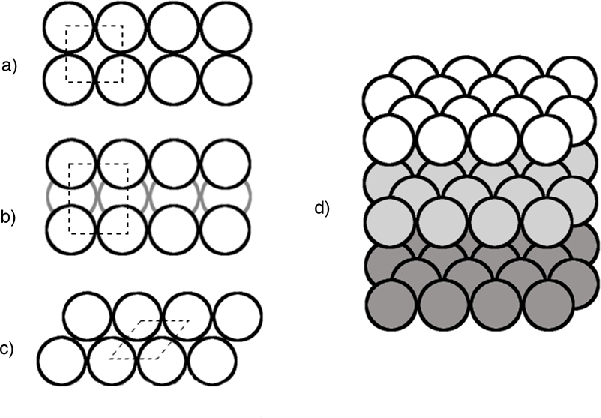
\includegraphics[width=\linewidth]{../figures/chap1/facets.pdf}
  \caption{On the left are displayed face-down views of common low-index facets
of metals (a) (100), (b) (110), and (c) (111). The dotted lines represent a
repeatable crystal unit on each facet. The light gray coloring in (b) is
illustrating the placement of that row of atoms behind the top and bottom row.
Facet (d) displays a (112) step edge. The darker shading represents separate
terraces that are displaced by one atomic height.}
\label{fig:facets}
\end{figure}

However, the presence of kinetic barriers coupled with the small size of
nanoparticles requires that not every atom on the surface will be part of a
(111) plane. As highlighted in Figure \ref{fig:facets}.d, one very common
defect observed on large crystals is that of step-edges. The (111) motif is
overwhelming present, however, there are also single atom height displacements
between plateaus. The edge atoms because of their undercoordination will
interact differently with adsorbates, potentially making those sites very
catalytically active. 

Nanoparticles and nanospheres especially have a large number of edge, kink, and
adatoms which are all of catalytic interest but are not seen on the low-index
surfaces.  However, the size of nanoparticles makes simulating them costly and
instead smaller surfaces with a large Miller index are used as a model for the
more complicated nanoparticles. Having a working knowledge of the displayed
low-energy structures is very important when considering how the metal will
interact with adsorbates because the strength of the adsorption will depend on
the displayed surfaced.


\subsubsection{Bimetallic and Supported Systems}
The displayed structure and binding properties of metal systems are directly
tied to their electronic structure and anything that perturbs the ideal system
will lead to deviations from bulk behavior. This deviation may be exactly what
is needed to tune a material for a certain catalytic process and significant
research has been directed at examining various bimetallic species including
heterogenous alloys, core-shell nanoparticles, and near-surface alloys.
Additionally, supported nanoparticles and metal surfaces can also be tuned
somewhat. 

By introducing another metal or a support that will donate or remove electron
density from the system, the electronic structure can be tuned for the desired
application. Figure \ref{fig:bimetallic} shows a number of ideal examples of
these types of systems. While synthesizing these systems can be extremely
challenging, the ability to specifically tune the catalysts for certain
reactions, resistance to poisoning\citep{Sharma:0ly, Yu:2013fr}, and cheaper
costs\citep{Li:0hl, Zhao:0qf} provides a strong impetus for the characterization
of these materials.

\begin{figure}[p!]
  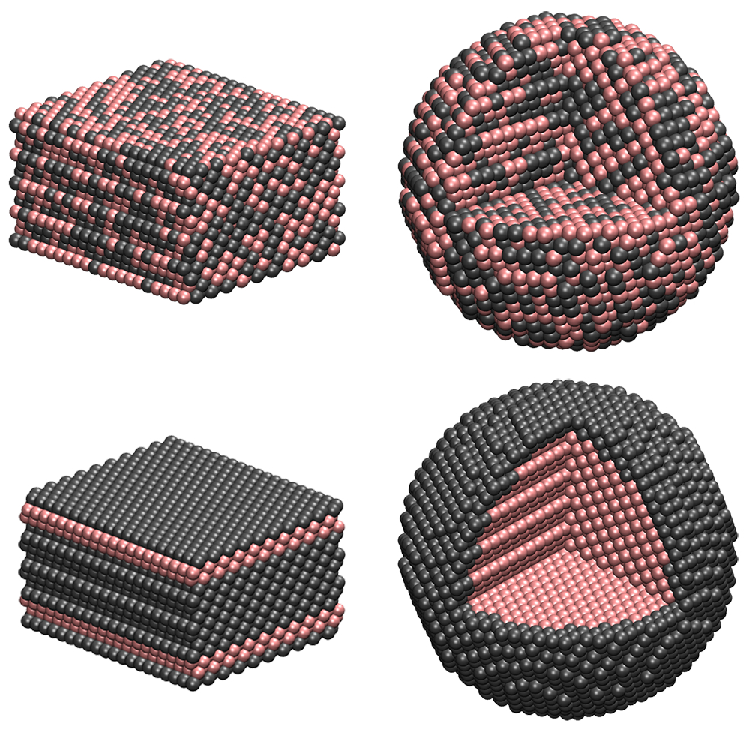
\includegraphics[width=\linewidth]{../figures/chap1/bimetallic.pdf}
\caption{The top two systems are Pd\textsubscript{0.5}Pt\textsubscript{0.5}
homogeneous alloys (Pd pink, Pt gray), with the left representing a (111) surface
and the right image depicting a 30~\AA\ nanosphere. The bottom left image
displays a near-surface alloy with two layers of Pd sandwiched between layers of
Pt while the right image shows a core-shell nanosphere with a small section cut
away to allow the thickness of the shell to be seen.}
\label{fig:bimetallic} 
\end{figure}

\subsection{Dynamics}
Metal self-interactions tend to be strong enough so that at room temperature
minimal movement of the metal atoms is observed. This is particularly true for
low-index facets since these surfaces tend to exist in relatively deep local
minima on the potential energy surface. However, these systems are also less
useful for applications, partially because of the stability of the surface
atoms. Many industrial processes make use of high-index or roughenend
nanopartciles so as to have a larger number of under \& over-coordinated
surface atoms, because these atoms tend to be more active for catalytic
processes.\citep{Calle-Vallejo:2015qq, Stephens:2011bv} This modification of
the local environment creates additional binding possiblities on the surface
and can also lead to easier adatom formation and surface mobility.
Additionally, the presence of adsorbates can also strongly affect the dynamics
of a metal surface because of the potential for strong interactions (primarily
repulsive) between adsorbates, which can effectively weaken the metal-metal
binding and allow for easier adatom formation.


\subsubsection{Diffusion \& Step-Wandering}
Barring macroscopic perturbations and the resultant large-scale modification of
a metal surface, {\em i.e.} ablation, mechanical-cleaving, etc. all movement on
surfaces ultimately involves the movement of adatoms. The two primary modes of
traversal can be distinguished by the adatoms moving independently, diffusion,
or in a concerted fashion, step-wandering. While it is helpful to divide these
two modes, they are in many ways coupled.  Independent adatom movement or
diffusion is more likely to be observed as it only requires one surface atom to
be ejected from a stable edge or terrace or upwards from a surface.  Since the
strength of metallic bonding is proportional to the number of nearest
neighbors, once an adatom is created and is seated on the surface, there is
often only a minimal energy barrier for the adatom to continue diffusing around
the surface.

The second main type of movement involves cooperative adatom diffusion and is
better described as entire step-edges ``wandering'' on the surface. This
wandering is ultimately a collection of ejection and readsorbtion events of
surface metal atoms but it is more helpful to look at the collective motion
than all of the individual motions. Specifically, reconstruction events tend to
involve the appearance or disappearance of step-edges as their presence tends
to raise the surface energy of a system while lowering their stability.

\section{Adsorbate Interactions on Metal Surfaces}
The majority of applications involving metals ultimately involve the metal
surface providing a favorable environment for some other reaction to occur,
whether that be oxidation of CO, production of \ce{H2} through a
water-gas-shift reaction, or some other mechanism that involves molecules
adsorbing to a surface. Having an accurate understanding of how adsorbates
interact with metal surfaces is thus of the utmost importance when attempting
to design more effective catalysts.

\subsection{Binding Sites}
While bulk metals are well described by their  high symmetry and formation of
electronic bands, surfaces break that symmetry and allow for rehybridization of
metallic orbitals to occur upon approach of adsorbates. While the idea is not
exact, thinking of surface metal atoms as possessing atomic {\em s, p, } and {\em d}
orbitals available for bonding as in regular molecular orbital theory can be
helpful. On a (111) surface there are three primary binding sites, the 1-fold
(atop), 2-fold (bridge), and 3-fold (hollow) sites, which are highlighted in
Figure \ref{fig:binding}. 

\begin{figure}[p!]
  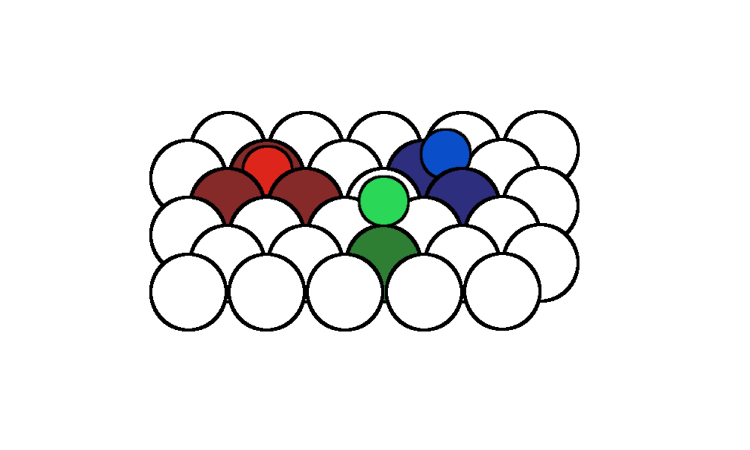
\includegraphics[width=\linewidth]{../figures/chap1/binding.pdf}
  \caption{The atop (green), bridge (blue), and three-fold hollow (red)
adsorption sites are the three most common binding sites for small molecules on
low-index surfaces. Depending on the energy levels of the adsorbate orbitals
that engage in bonding there will be varying preferences for binding sites.}
\label{fig:binding}
\end{figure}

As an illustrative example, carbon monoxide on platinum (111) has been studied
extensively\citep{Ertl:1977cg, Kelemen:1979ad, Yeo:1997th, Wong:1991ta, Feibelman:2001qa, Deshlahra:2009wu,
Deshlahra:2012aa} and is often used as a model for molecular adsorption on
metal surfaces.  Hoffman {\em et al.} utilizing the extended H\"uckel
method\citep{Wong:1991ta} were able to calculate the overlap population between
the CO and Pt orbitals and how they changed depending on which binding site
they had placed CO at. As a specific example, when CO was placed in the atop
position, its 5$\sigma$ orbital only interacted with 3 of Pt's frontier
orbitals, the 6s, 5p\textsubscript{z}, and
3d\textsubscript{z\textsuperscript{2}}. However, when they placed CO into the
3-fold hollow site, all nine surface bands showed at least some overlap with
CO's 5$\sigma$ orbital. While this type of analysis has become more mainstream,
predictions of preferred binding sites are still incredibly complicated,
especially since they are often coverage-dependent.

\subsection{Coverage Dependence}
While there might be one preferred binding site for a single adsorbate on a
metal surface, the presence of strong adsorbate-adsorbate interactions can lead
to deviations from expected behavior. Again looking to CO on Pt (111), at low
coverages ( $<$ 0.25 ML), CO has been observed to bind primarily to atop sites.
As the coverage increases however, adsorbate-adsorbate repulsions cause the
preferred binding to change to a mix of atop and bridge sites.\citep{Deshlahra:2012aa} Typically,
adsorbate-adsorbate interactions are repulsive which results in weaker overall
binding and can induce strain in the metal surface making it easier for the
surface to overcome potential barriers to restructuring.

In certain circumstances adsorbate-adsorbate interactions can be cooperative.
Scneider {\em et al.} performed DFT calculations of CO on Pt (111) at 0.5 ML
coverage and observed that the preferred binding was a mix of atop and bridge
sites.\citep{Deshlahra:2012aa} This configuration was a result of favorable
dipole-dipole interactions that result due to non-equivalent $2\pi^*$
back-donation from the Platinum to the CO.


\subsubsection{Adsorbate Patterning}
%Image of particles adsorbed on the surface
The complex interactions between adsorbates on a surface can often lead to
large-scale patterning which can be observed with XPS (X-Ray Photoelectron
Spectroscopy), LEED (Low Energy Electron Diffraction), and other experimental
techniques. The preferred binding sites, as mentioned earlier, are dependent on
coverage, since the presence of bound adsorbates affects the energy levels of
the surface. Thus, at different coverages, different patterns are observed. For
example, \ce{CO} on \ce{Pd} at $\theta = 1/3$ coverage tends to be
arranged in a $(\sqrt{3}\times\sqrt{3})\textrm{R}30^o$ pattern. However, raising the coverage to a
half-monolayer, $\theta = 1/2$, causes the experimentally observed patterning to change to a c$(4\times2)$
pattern. If the coverage is further increased to three-quarters monolayer, $\theta = 3/4$, 
the preferred pattern is a $(2\times2)$ pattern.\citep{Guo:1989aa} These patterns are
all diagrammed in Figure \ref{fig:patterns}.

\begin{figure}[p!]
\centering
  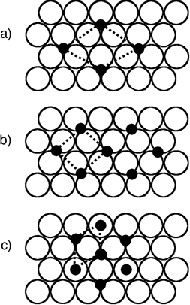
\includegraphics[width=0.5\linewidth]{../figures/chap1/pattern.pdf}
  \caption{Adsorbate patterns of CO on Pd (111), (a)
$(\sqrt{3}\times\sqrt{3})\textrm{R}30^o$, (b) c$(4\times2)$, (c) $(2\times2)$.}
\label{fig:patterns}
\end{figure}

A good model of the adsorbate and adsorbate-metal interactions should be able
to capture some of these different patterns; however, capturing every possible
arrangement is incredibly complex and beyond the scope of most
investigations.

\section{Adsorbate Induced Reconstructions}
% Studies done on clean metal surfaces tend to suffer from pressure and temperature gaps
% high pressure xps, stm, spin echo helium bombardment provide some ways to mimic the environment of industrial catalysts
% Difficult to determine mechanisms because of time and spacial resolution
% DFT good at calculating relative energies for small systems, but the size of these reconstructions makes calculations expensive
% mol dyn. allows us to explore the interactions that lead to adsorbate-induced reconstructions

While metal surfaces often remain stable even when the environment is
perturbed, some situations can arise where the presence of adsorbates
sufficiently modify the potential energy surface so that a new facet is
energetically favored. This situation might even be commonplace, but altering
the potential energy surface does not ensure that a reconstruction will take
place. The system must also be able to overcome any kinetic barriers that would
trap the surface in a local minima.  For systems that are started far from a
low surface energy state, ({\em i.e.} nanoparticles and
roughened surfaces) the introduction of adsorbates will likely lead to a
restructuring to a lower-energy structure. 

The time and length scales of these reconstruction processes can vary widely
and while current experimental techniques are able to observe and identify the
reconstructions, they are often unable to identify the actual mechanisms of
restructuring which could prove crucial in designing better catalysts.

\subsection{Refaceting}
If a bulk crystal is cut at too large of an angle, there may be a strong
driving force to refacet. Barring large kinetic barriers that keep certain
facets as metastable states, a surface facet will desire to reconstruct so long as the
orientation $\hat{n}_0$ of the facet is conserved and the overall tension
$\gamma$ is reduced as shown in the relations derived by Herring\citep{Herring:1951ta}, where
$A_i$ is the area of the surface of orientation $\hat{n}_i$.

\begin{equation}
A_0\hat{n}_0 = A_a\hat{n}_a + A_b\hat{n}_b \\
A_0\gamma(\hat{n}_0) > A_a\gamma(\hat{n}_a) + A_b\gamma(\hat{n}_b)
\end{equation}

This restructuring generally only occurs in the forward direction and while the
presence of adsorbates can be sufficient to induce this reconstruction, a
temperature increase can also allow this to refaceting to occur since it is
most likely that there is simply a kinetic barrier that must be overcome.\citep{Williams:1994aa, Jeong:1999ev} 

\subsubsection{Doubling}
Work by Tao {\it et al.} on a \ce{Pt} (557) surface exposed to \ce{CO} observed
a reversible reconstruction event that was directly dependent on the presence
of \ce{CO} in the system.\citep{Tao:2011aa} When \ce{CO} was introduced the step-edges doubled,
but upon removal of the \ce{CO} the original (557) motif was recovered. This
reversible reconstruction strongly implies that the presence of \ce{CO}
temporarily modified the potential energy surface to prefer a new ground state
structure; however, the exact mechanism of this reconstruction was not deduced
at the time. This dissertation originally started as an attempt to model this
system and attempt to provide insights into the mechanism of reconstruction. 

\subsection{Island Formation and Sintering}
Since catalytic reactions typically only occur at the surface of metals, significant
research has been devoted to increasing the surface area to bulk ratio of metal
catalysts, either through catalyst supports, high-index nanostructures, or
bimetallic near-surface alloys. While these systems are typically stable at low
temperatures and pressures, significant perturbations can lead to what is
effectively sintering or island-formation of one of the metals on the surface.
The interplay of surface energies and adsorbate interactions on two or more
metal surfaces allows for the creation of incredibly tuned catalysts.


\chapter{MOLECULAR DYNAMICS SIMULATIONS OF THE SURFACE RECONSTRUCTIONS OF PT(557) AND AU(557) UNDER EXPOSURE TO CO}


%\begin{abstract}
%  The mechanism and dynamics of surface reconstructions of Pt(557) and
%  Au(557) exposed to various coverages of carbon monoxide (CO) were
%  investigated using molecular dynamics simulations.  Metal-CO
%  interactions were parameterized from experimental data and
%  plane-wave Density Functional Theory (DFT) calculations.  The large
%  difference in binding strengths of the Pt-CO and Au-CO interactions
%  was found to play a significant role in step-edge stability and
%  adatom diffusion constants.  Various mechanisms for CO-mediated step
%  wandering and step doubling were investigated on the Pt(557)
%  surface.  We find that the energetics of CO adsorbed to the surface
%  can explain the step-doubling reconstruction observed on Pt(557) and
%  the lack of such a reconstruction on the Au(557) surface.  However,
%  more complicated reconstructions into triangular clusters that have
%  been seen in recent experiments were not observed in these
%  simulations.
%\end{abstract}

%\newpage


\section{Introduction}
% Importance: catalytically active metals are important
% 	Sub: Knowledge of how their surface structure affects their ability to catalytically facilitate certain reactions is growing, but is more reactionary than predictive
%	Sub: Designing catalysis is the future, and will play an important role in numerous processes (ones that are currently seen to be impractical, or at least inefficient)
% Theory can explore temperatures and pressures which are difficult to work with in experiments
%	Sub: Also, easier to observe what is going on and provide reasons and explanations
%

Industrial catalysts usually consist of small particles that exhibit a
high concentration of steps, kink sites, and vacancies at the edges of
the facets.  These sites are thought to be the locations of catalytic
activity.\citep{ISI:000083038000001,ISI:000083924800001} There is now
significant evidence that solid surfaces are often structurally,
compositionally, and chemically modified by reactants under operating
conditions.\citep{Tao2008,Tao:2010,Tao2011} The coupling between
surface oxidation states and catalytic activity for CO oxidation on
Pt, for instance, is widely documented.\citep{Ertl08,Hendriksen:2002}
Despite the well-documented role of these effects on reactivity, the
ability to capture or predict them in atomistic models is somewhat
limited.  While these effects are perhaps unsurprising on the highly
disperse, multi-faceted nanoscale particles that characterize
industrial catalysts, they are manifest even on ordered, well-defined
surfaces. The Pt(557) surface, for example, exhibits substantial and
reversible restructuring under exposure to moderate pressures of
carbon monoxide.\citep{Tao:2010}

This work is an investigation into the mechanism and timescale for the
Pt(557) \& Au(557) surface restructuring using molecular simulation.
Since the dynamics of the process are of particular interest, we
employ classical force fields that represent a compromise between
chemical accuracy and the computational efficiency necessary to
simulate the process of interest.  Since restructuring typically
occurs as a result of specific interactions of the catalyst with
adsorbates, in this work, two metal systems exposed to carbon monoxide
were examined. The Pt(557) surface has already been shown to undergo a
large scale reconstruction under certain conditions.\citep{Tao:2010}
The Au(557) surface, because of weaker interactions with CO, is less
likely to undergo this kind of reconstruction. However, Peters {\it et
  al}.\citep{Peters:2000} and Piccolo {\it et al}.\citep{Piccolo:2004}
have both observed CO-induced modification of reconstructions to the
Au(111) surface. Peters {\it et al}. observed the Au(111)-($22 \times
\sqrt{3}$) ``herringbone'' reconstruction relaxing slightly under CO
adsorption. They argued that only a few Au atoms become adatoms,
limiting the stress of this reconstruction, while allowing the rest to
relax and approach the ideal (111) configuration.  Piccolo {\it et
  al}. on the other hand, saw a more significant disruption of the
Au(111)-($22 \times \sqrt{3}$) herringbone pattern as CO adsorbed on
the surface. Both groups suggested that the preference CO shows for
low-coordinated Au atoms was the primary driving force for the
relaxation.  Although the Au(111) reconstruction was not the primary
goal of our work, the classical models we have fit may be of future
use in simulating this reconstruction.

%Platinum molecular dynamics
%gold molecular dynamics

\section{Simulation Methods}
The challenge in modeling any solid/gas interface is the development
of a sufficiently general yet computationally tractable model of the
chemical interactions between the surface atoms and adsorbates.  Since
the interfaces involved are quite large (10$^3$ - 10$^4$ atoms), have
many electrons, and respond slowly to perturbations, {\it ab initio}
molecular dynamics
(AIMD),\citep{KRESSE:1993ve,KRESSE:1993qf,KRESSE:1994ul} Car-Parrinello
methods,\citep{CAR:1985bh,Izvekov:2000fv,Guidelli:2000fy} and quantum
mechanical potential energy surfaces remain out of reach.
Additionally, the ``bonds'' between metal atoms at a surface are
typically not well represented in terms of classical pairwise
interactions in the same way that bonds in a molecular material are,
nor are they captured by simple non-directional interactions like the
Coulomb potential.  For this work, we have used classical molecular
dynamics with potential energy surfaces that are specifically tuned
for transition metals.  In particular, we used the EAM potential for
Au-Au and Pt-Pt interactions.\citep{Foiles86} The CO was modeled using
a rigid three-site model developed by Straub and Karplus for studying
photodissociation of CO from myoglobin.\citep{Straub} The Au-CO and
Pt-CO cross interactions were parameterized as part of this work.
  
\subsection{Metal-metal interactions}
Many of the potentials used for modeling transition metals are based
on a non-pairwise additive functional of the local electron
density. The embedded atom method (EAM) is perhaps the best known of
these
methods,\citep{Daw84,Foiles86,Johnson89,Daw89,Plimpton93,Voter95a,Lu97,Alemany98}
but other models like the Finnis-Sinclair\citep{Finnis84,Chen90} and
the quantum-corrected Sutton-Chen method\citep{QSC,Qi99} have simpler
parameter sets. The glue model of Ercolessi {\it et
  al}.\citep{Ercolessi88} is among the fastest of these density
functional approaches. In all of these models, atoms are treated as a
positively charged core with a radially-decaying valence electron
distribution. To calculate the energy for embedding the core at a
particular location, the electron density due to the valence electrons
at all of the other atomic sites is computed at atom $i$'s location,
\begin{equation*}
\bar{\rho}_i = \sum_{j\neq i} \rho_j(r_{ij})
\end{equation*}
Here, $\rho_j(r_{ij})$ is the function that describes the distance
dependence of the valence electron distribution of atom $j$. The
contribution to the potential that comes from placing atom $i$ at that
location is then
\begin{equation*}
V_i =  F[ \bar{\rho}_i ]  + \sum_{j \neq i} \phi_{ij}(r_{ij})
\end{equation*}
where $F[ \bar{\rho}_i ]$ is an energy embedding functional, and
$\phi_{ij}(r_{ij})$ is a pairwise term that is meant to represent the
repulsive overlap of the two positively charged cores.  

% The {\it modified} embedded atom method (MEAM) adds angular terms to
% the electron density functions and an angular screening factor to the
% pairwise interaction between two
% atoms.\citep{BASKES:1994fk,Lee:2000vn,Thijsse:2002ly,Timonova:2011ve}
% MEAM has become widely used to simulate systems in which angular
% interactions are important (e.g. silicon,\citep{Timonova:2011ve} bcc
% metals,\citep{Lee:2001qf} and also interfaces.\citep{Beurden:2002ys})
% MEAM presents significant additional computational costs, however.

The EAM, Finnis-Sinclair, and the Quantum Sutton-Chen (QSC) potentials
have all been widely used by the materials simulation community for
simulations of bulk and nanoparticle
properties,\citep{Chui:2003fk,Wang:2005qy,Medasani:2007uq,mishin99:_inter}
melting,\citep{Belonoshko00,sankaranarayanan:155441,Sankaranarayanan:2005lr}
fracture,\citep{Shastry:1996qg,Shastry:1998dx,mishin01:cu} crack
propagation,\citep{BECQUART:1993rg,Rifkin1992} and alloying
dynamics.\citep{Shibata:2002hh,mishin02:b2nial,zope03:tial_ap,mishin05:phase_fe_ni}
One of EAM's strengths is its sensitivity to small changes in
structure. This is due to the inclusion of up to the third nearest
neighbor interactions during fitting of the parameters.\citep{Voter95a}
In comparison, the glue model of Ercolessi {\it et
  al}.\citep{Ercolessi88} was only parameterized to include
nearest-neighbor interactions, EAM is a suitable choice for systems
where the bulk properties are of secondary importance to low-index
surface structures. Additionally, the similarity of EAM's functional
treatment of the embedding energy to standard density functional
theory (DFT) makes fitting DFT-derived cross potentials with
adsorbates somewhat easier.

\subsection{Carbon Monoxide model}
Previous explanations for the surface rearrangements center on the
large linear quadrupole moment of carbon monoxide.\citep{Tao:2010} We
used a model first proposed by Karplus and Straub to study the
photodissociation of CO from myoglobin because it reproduces the
quadrupole moment well.\citep{Straub} The Straub and Karplus model
treats CO as a rigid three site molecule with a massless
charge-carrying ``M'' site at the center of mass. The geometry and
interaction parameters are reproduced in Table~\ref{tab:CO}. The
effective dipole moment, calculated from the assigned charges, is
still small (0.35 D) while the linear quadrupole (-2.40 D~\AA) is
close to the experimental (-2.63 D~\AA)\citep{QuadrupoleCO} and quantum
mechanical predictions (-2.46 D~\AA)\citep{QuadrupoleCOCalc}.

%CO Table
\begin{table}[H]
\caption{POSITIONS, LENNARD-JONES PARAMETERS ($\sigma$ AND $\epsilon$), AND
CHARGES FOR CO-CO INTERACTIONS}
\centering
\begin{threeparttable}
%  \caption{Positions, Lennard-Jones parameters ($\sigma$ and
%    $\epsilon$), and charges for CO-CO 
%    interactions. Distances are in \AA, energies are 
%    in kcal/mol, and charges are in atomic units.  The CO model
%    from Ref.\bibpunct{}{}{,}{n}{}{,}
%    \protect\citep{Straub} was used without modification.}
\centering
\begin{tabular}{ c  c  ccc }
\hline \hline
&  {\it z}\tnote{a} & $\sigma$\tnote{a} & $\epsilon$\tnote{b} & q\tnote{c}\\
\hline
\textbf{C} & -0.6457 &  3.83 & 0.0262   &   -0.75 \\
\textbf{O} &  0.4843 &  3.12 &  0.1591  &   -0.85 \\
\textbf{M} & 0.0 & -  &  -  &    1.6 \\
\hline \hline
\end{tabular}
\begin{tablenotes}
  \item The CO model from Ref.\citep{Straub} was used without modification.
  \item[a] Distances are in \AA.
  \item[b] Energies are in kcal/mol.
  \item[c] Charges are in a.u.
\end{tablenotes}
\end{threeparttable}
\label{tab:CO}
\end{table}

\subsection{Cross-Interactions between the metals and carbon monoxide}

Since the adsorption of CO onto a Pt surface has been the focus
of much experimental \citep{Yeo, Hopster:1978, Ertl:1977, Kelemen:1979}
and theoretical work
\citep{Beurden:2002ys,Pons:1986,Deshlahra:2009,Feibelman:2001,Mason:2004}
there is a significant amount of data on adsorption energies for CO on
clean metal surfaces. An earlier model by Korzeniewski {\it et
  al.}\citep{Pons:1986} served as a starting point for our fits. The parameters were
modified to ensure that the Pt-CO interaction favored the atop binding
position on Pt(111). These parameters are reproduced in Table~\ref{tab:co_parameters}.
The modified parameters yield binding energies that are slightly higher
than the experimentally-reported values as shown in Table~\ref{tab:co_energies}. Following Korzeniewski
{\it et al}.,\citep{Pons:1986} the Pt-C interaction was fit to a deep
Lennard-Jones interaction to mimic strong, but short-ranged, partial
binding between the Pt $d$ orbitals and the $\pi^*$ orbital on CO. The
Pt-O interaction was modeled with a Morse potential with a large
equilibrium distance, ($r_o$).  These choices ensure that the C is preferred
over O as the surface-binding atom. In most geometries, the Pt-O parameterization contributes a weak
repulsion which favors the atop site.  The resulting potential-energy
surface suitably recovers the calculated Pt-C separation length
(1.6~\AA)\citep{Beurden:2002ys} and affinity for the atop binding
position.\citep{Deshlahra:2012, Hopster:1978}

%where did you actually get the functionals for citation?
%scf calculations, so initial relaxation was of the four layers, but two layers weren't kept fixed, I don't think
%same cutoff for slab and slab + CO ? seems low, although feibelmen had values around there...
The Au-C and Au-O cross-interactions were also fit using Lennard-Jones and
Morse potentials, respectively, to reproduce Au-CO binding energies.
The limited experimental data for CO adsorption on Au required refining the fits against plane-wave DFT calculations.
Adsorption energies were obtained from gas-surface DFT calculations with a
periodic supercell plane-wave basis approach, as implemented in the
Quantum ESPRESSO package.\citep{QE-2009} Electron cores were
described with the projector augmented-wave (PAW)
method,\citep{PhysRevB.50.17953,PhysRevB.59.1758} with plane waves
included to an energy cutoff of 20 Ry. Electronic energies are
computed with the PBE implementation of the generalized gradient
approximation (GGA) for gold, carbon, and oxygen that was constructed
by Rappe, Rabe, Kaxiras, and Joannopoulos.\citep{Perdew_GGA,RRKJ_PP}
In testing the Au-CO interaction, Au(111) supercells were constructed of four layers of 4
Au x 2 Au surface planes and separated from vertical images by six
layers of vacuum space. The surface atoms were all allowed to relax 
before CO was added to the system. Electronic relaxations were 
performed until the energy difference between subsequent steps 
was less than $10^{-8}$ Ry.   Nonspin-polarized supercell calculations 
were performed with a 4~x~4~x~4 Monkhorst-Pack {\bf k}-point sampling of the first Brillouin
zone.\citep{Monkhorst:1976} The relaxed gold slab was
then used in numerous single point calculations with CO at various
heights (and angles relative to the surface) to allow fitting of the
empirical force field.

%Hint at future work
The parameters employed for the metal-CO cross-interactions in this work 
are shown in Table~\ref{tab:co_parameters} and the binding energies on the 
(111) surfaces are displayed in Table~\ref{tab:co_energies}.  Charge transfer
and polarization are neglected in this model, although these effects could have 
an effect on binding energies and binding site preferences.

%Table  of Parameters
%Pt Parameter Set 9
%Au Parameter Set 35
\begin{table}[H]
  \caption{PARAMETERS FOR THE METAL-CO CROSS-INTERACTIONS}
%  \caption{Parameters for the metal-CO cross-interactions. Metal-C
%    interactions are modeled with Lennard-Jones potentials, while the
%    metal-O interactions were fit to broad Morse
%    potentials.  Distances are given in \AA~and energies in kcal/mol. }
\centering
\begin{threeparttable}
\begin{tabular}{  c   cc   c  ccc }
\hline \hline
 &  $\sigma$\tnote{a} & $\epsilon$\tnote{b} & & $r$\tnote{a} & $D$\tnote{b} & $\gamma$ (\AA$^{-1}$) \\
\hline
\textbf{Pt-C} & 1.3 & 15  & \textbf{Pt-O} & 3.8 & 3.0 & 1 \\
\textbf{Au-C} & 1.9 & 6.5  & \textbf{Au-O} & 3.8 & 0.37 & 0.9\\
\hline \hline
\end{tabular}
\begin{tablenotes}
  \item Metal-C interactions are modeled with Lennard-Jones potentials, while the metal-O interactions were fit to broad Morse potentials.
  \item[a] Distances are given in \AA
  \item[b] Energies are given in kcal/mol
\end{tablenotes}
\end{threeparttable}
\label{tab:co_parameters}
\end{table}

%Table of energies
\begin{table}[H]
%  \caption{Adsorption energies for a single CO at the atop site on M(111) using
%the potentials described in this work.  All values are in eV.}
\caption{ADSORPTION ENERGIES FOR CO ON M(111)}
\centering
\begin{threeparttable}
\begin{tabular}{ c  cc }
  \hline \hline
  & Calculated\tnote{a} & Experimental\tnote{a} \\
  \hline
%  \multirow{2}{*}{\textbf{Pt-CO}} & \multirow{2}{*}{-1.81} & -1.4 \bibpunct{}{}{,}{n}{}{,}
%  (Ref. \protect\citep{Kelemen:1979}) \\
% & &  -1.9 \bibpunct{}{}{,}{n}{}{,} (Ref. \protect\citep{Yeo}) \\ \hline
%  \textbf{Au-CO} & -0.39 & -0.40 \bibpunct{}{}{,}{n}{}{,}  (Ref. \protect\citep{TPDGold}) \\
  \multirow{2}{*}{\textbf{Pt-CO}} & \multirow{2}{*}{-1.81} & -1.4
  Ref. \citep{Kelemen:1979} \\
 & &  -1.9 Ref. \citep{Yeo} \\ \hline
  \textbf{Au-CO} & -0.39 & -0.40 Ref. \citep{TPDGold} \\
  \hline \hline
\end{tabular}
\begin{tablenotes}
  \item The adsorption energies were calculated for a single CO molecule
adsorbed vertically at an atop binding site on a (111) metal surface using the
potentials described in this work 
  \item[a] Adsorption energies are given in eV
\end{tablenotes}
\end{threeparttable}
\label{tab:co_energies}
\end{table}


\subsection{Force field validation}
The CO-Pt cross interactions were compared directly to DFT results
found in the supporting information of reference
\citep{Tao:2010}. These energies are
estimates of the degree of stabilization provided to double-layer
reconstructions of the M(557) surface by an overlayer of CO molecules
in a $c (2 \times 4)$ pattern.  To make the comparison, five atom
thick metal slabs of both Pt and Au displaying the (557) facet were
constructed.  Double-layer (reconstructed) systems were created using
six atomic layers where enough of a layer was removed from both
exposed (557) facets to create the double step.  In all cases, the
metal slabs contained 480 atoms and were minimized using steepest
descent under the EAM force field. Both the bare metal slabs and slabs
with 50\% carbon monoxide coverage (arranged in the $c (2 \times 4)$
pattern) were used.  The systems are periodic along and perpendicular
to the step-edge axes with a large vacuum above the displayed (557)
facet.

Energies computed using our force field are displayed in Table
~\ref{tab:steps}.  The relative energies are calculated as
$E_{relative} = E_{system} - E_{M(557)-S} - N_{CO}*E_{M-CO}(r)$, where
$E_{M(557)-S}$ is the energy of a clean (557) surface. $N_{CO}$ is the
number of CO molecules present on the surface.  In the $c (2 \times
4)$ patterning, the CO molecules relax to an average separation, $r$,
from the nearest surface metal atom.  $E_{M-CO}(r)$ is taken as the
energy of a single CO molecule on a flat M(111) surface at a distance
$r$ from a metal atop site.  These energies correspond to -1.8 eV for
CO-Pt and -0.39 eV for CO-Au. 

One important note is that the $c (2 \times 4)$ patterning on the
stepped surfaces yields a slightly larger M-CO separation than one
would find on a clean (111) surface. On a clean Pt(111) surface, for
example, the optimized geometry has a C-Pt distance of 1.53~\AA
(corresponding to a binding energy of -1.83 eV).  On the double-layer
reconstruction and the single (557) step, the half monolayer optimizes
to C-Pt separations of 1.58-1.60~\AA, respectively.  Although this
difference seems quite small, there are notable consequences for
$E_{Pt-CO}(r)$ which then takes values from -1.815 eV to -1.8 eV.

For platinum, the bare double layer reconstruction is less stable than
the bare (557) step by about 0.25 kcal/mol per Pt atom. However,
addition of carbon monoxide changes the relative energetics of the two
systems. This is a quite dramatic shift, $\Delta\Delta E$ (the change
in energy for going from single to double-layer structures upon
addition of a CO layer) shifts by -0.5~kcal/mol per Pt atom. This
result is in qualitative agreement with the DFT calculations in
reference \citep{Tao:2010}, which
also showed that the addition of CO leads to a reversal in stability.

The gold systems show a smaller energy difference between the clean
single and double layers. Upon addition of CO, the single step surface
is much more stable than the double-layer reconstruction.  However,
the CO-Au binding energy is much weaker, so at operating temperatures,
the actual coverage by CO will be much lower than the 50\% coverage
afforded by the $c (2 \times 4)$ pattern, so single-point energy
comparisons are not as helpful.

%Table of single step double step calculations
\begin{table}
\caption{RELATIVE ENERGIES OF (S)INGLE M(557) AND (D)OUBLE-STEP RECONSTRUCTIONS}
%  \caption{Relative energies (in kcal/mol) of (S)ingle M(557) and
%    (D)ouble-step reconstructions. 50\% coverage by CO in a  $c(2
%    \times 4)$ pattern stabilizes the D-reconstructed Pt(557)
%    surface, but leaves the single-step Au(557) as the more stable structure.}
\centering
\begin{threeparttable}
\centering
\begin{tabular}{  c   c   c   c   c  }
\hline \hline
Step & $N_{M}$ & $N_{CO}$ & Relative Energy & $\Delta E / N_{M}$ \\
\hline
Pt(557)-S & 480 & 0  &  0 & 0 \\
Pt(557)-D & 480 & 0  &  119.788 & 0.2495 \\
Pt(557)-S & 480 & 40 &  -109.734 & -0.2286 \\
Pt(557)-D & 480 & 48 &  -110.039 & -0.2292 \\
\hline
Au(557)-S & 480 & 0  &  0 & 0  \\
Au(557)-D & 480 & 0  &  83.853 & 0.1747 \\
Au(557)-S & 480 & 40 &  -253.604 & -0.5283 \\
Au(557)-D & 480 & 48 &  -156.150 & -0.3253 \\
\hline \hline
\end{tabular}
\begin{tablenotes}
  \item The presence of a 50\% coverage of CO in a $c(2\times 4)$ pattern stabilizes the D-reconstructed Pt(557) surface, but leaves the S-unreconstructed Au(557) as the more stable structure
  \item[a] Energies are in kcal/mol
\end{tablenotes}
\end{threeparttable}
\label{tab:steps}
\end{table}

Qualitatively, our classical force field for the metal-CO cross
interactions reproduces the results predicted by DFT studies in
reference \citep{Tao:2010}. Addition
of polarization effects, both in the CO and in the metal surfaces,
could make the model significantly more accurate.  For example,
because of the relatively large fixed charges, the current model will
be unable to reproduce coverages in excess of 50\% without forming an
inverted CO second layer on the surface.  The M-CO cross interactions
would also be more accurate if they included the direct interactions
between charges on the CO and their image charges inside the metal
slab. These polarization effects have been shown to play an important
role,\citep{Deshlahra:2012} and would be one way of improving the
numerical agreement with quantum mechanical calculations.

\subsection{Pt(557) and Au(557) metal interfaces}
Our Pt system is an orthorhombic periodic box of dimensions
54.482~x~50.046~x~120.88~\AA, while our Au system has 
dimensions of 57.4~x~51.9285~x~100~\AA. The metal slabs 
are 9 and 8 atoms deep respectively, corresponding to a slab 
thickness of $\sim$21~\AA~ for Pt and $\sim$19~\AA~for Au.
The systems are arranged in a FCC crystal that have been cut
along the (557) plane so that they are periodic in the {\it x} and
{\it y} directions, and have been oriented to expose two aligned
(557) cuts along the extended {\it z}-axis.  Simulations of the 
bare metal interfaces at temperatures ranging from 300~K to
1200~K were performed to confirm the relative
stability of the surfaces without a CO overlayer.  

The different bulk melting temperatures predicted by EAM
(1345~$\pm$~10~K for Au\citep{Au:melting} and $\sim$~2045~K for
Pt\citep{Pt:melting}) suggest that any reconstructions should happen at
different temperatures for the two metals.  The bare Au and Pt
surfaces were initially run in the canonical (NVT) ensemble at 800~K
and 1000~K respectively for 100 ps. The two surfaces were relatively
stable at these temperatures when no CO was present, but experienced
increased surface mobility on addition of CO. Each surface was then
dosed with different concentrations of CO that was initially placed in
the vacuum region.  Upon full adsorption, these concentrations
correspond to 0\%, 5\%, 25\%, 33\%, and 50\% surface coverage. Higher
coverages resulted in the formation of a double layer of CO, which
introduces artifacts that are not relevant to (557) reconstruction.
Because of the difference in binding energies, nearly all of the CO
was bound to the Pt surface, while the Au surfaces often had a
significant CO population in the gas phase.  These systems were
allowed to reach thermal equilibrium (over 5~ns) before being run in
the microcanonical (NVE) ensemble for data collection. All of the
systems examined had at least 40~ns in the data collection stage,
although simulation times for some Pt of the systems exceeded 200~ns.
Simulations were carried out using the open source molecular dynamics
package, OpenMD.\citep{Ewald,OOPSE,openmd}


% RESULTS
%
\section{Results}
\subsection{Structural remodeling}
The bare metal surfaces experienced minor roughening of the step-edge
because of the elevated temperatures, but the (557) face was stable
throughout the simulations. The surfaces of both systems, upon dosage
of CO, began to undergo extensive remodeling that was not observed in
the bare systems. Reconstructions of the Au systems were limited to
breakup of the step-edges and some step wandering. The lower coverage
Pt systems experienced similar step edge wandering but to a greater
extent. The 50\% coverage Pt system was unique among our simulations
in that it formed well-defined and stable double layers through step
coalescence, similar to results reported by Tao {\it et
  al}.\citep{Tao:2010}

\subsubsection{Step wandering}
The bare surfaces for both metals showed minimal step-wandering at
their respective temperatures. As the CO coverage increased however,
the mobility of the surface atoms, described through adatom diffusion
and step-edge wandering, also increased.  Except for the 50\% Pt
system where step coalescence occurred, the step-edges in the other
simulations preferred to keep nearly the same distance between steps
as in the original (557) lattice, $\sim$13\AA~for Pt and
$\sim$14\AA~for Au.  Previous work by Williams {\it et
  al}.\citep{Williams:1991, Williams:1994} highlights the repulsion
that exists between step-edges even when no direct interactions are
present in the system. This repulsion is caused by an entropic barrier
that arises from the fact that steps cannot cross over one
another. This entropic repulsion does not completely define the
interactions between steps, however, so it is possible to observe step
coalescence on some surfaces.\citep{Williams:1991} The presence and
concentration of adsorbates, as shown in this work, can affect
step-step interactions, potentially leading to a new surface structure
as the thermodynamic equilibrium.

\subsubsection{Double layers}
Tao {\it et al}.\citep{Tao:2010} have shown experimentally that the
Pt(557) surface undergoes two separate reconstructions upon CO
adsorption.  The first involves a doubling of the step height and
plateau length.  Similar behavior has been seen on a number of
surfaces at varying conditions, including Ni(977) and
Si(111).\citep{Williams:1994,Williams:1991,Pearl} Of the two systems we
examined, the Pt system showed a greater propensity for reconstruction
because of the larger surface mobility and the greater extent of step
wandering.  The amount of reconstruction was strongly correlated to
the amount of CO adsorbed upon the surface.  This appears to be
related to the effect that adsorbate coverage has on edge breakup and
on the surface diffusion of metal adatoms. Only the 50\% Pt surface
underwent the doubling seen by Tao {\it et al}.\citep{Tao:2010} within
the time scales studied here.  Over a longer time scale (150~ns) two
more double layers formed on this surface. Although double layer
formation did not occur in the other Pt systems, they exhibited more
step-wandering and roughening compared to their Au counterparts. The
50\% Pt system is highlighted in Figure \ref{fig:reconstruct} at
various times along the simulation showing the evolution of a double
layer step-edge.

The second reconstruction observed by Tao {\it et al}.\citep{Tao:2010}
involved the formation of triangular clusters that stretched across
the plateau between two step-edges. Neither of the simulated metal
interfaces, within the 40~ns time scale or the extended time of 150~ns
for the 50\% Pt system, experienced this reconstruction.

%Evolution of surface
\begin{figure}[p!]
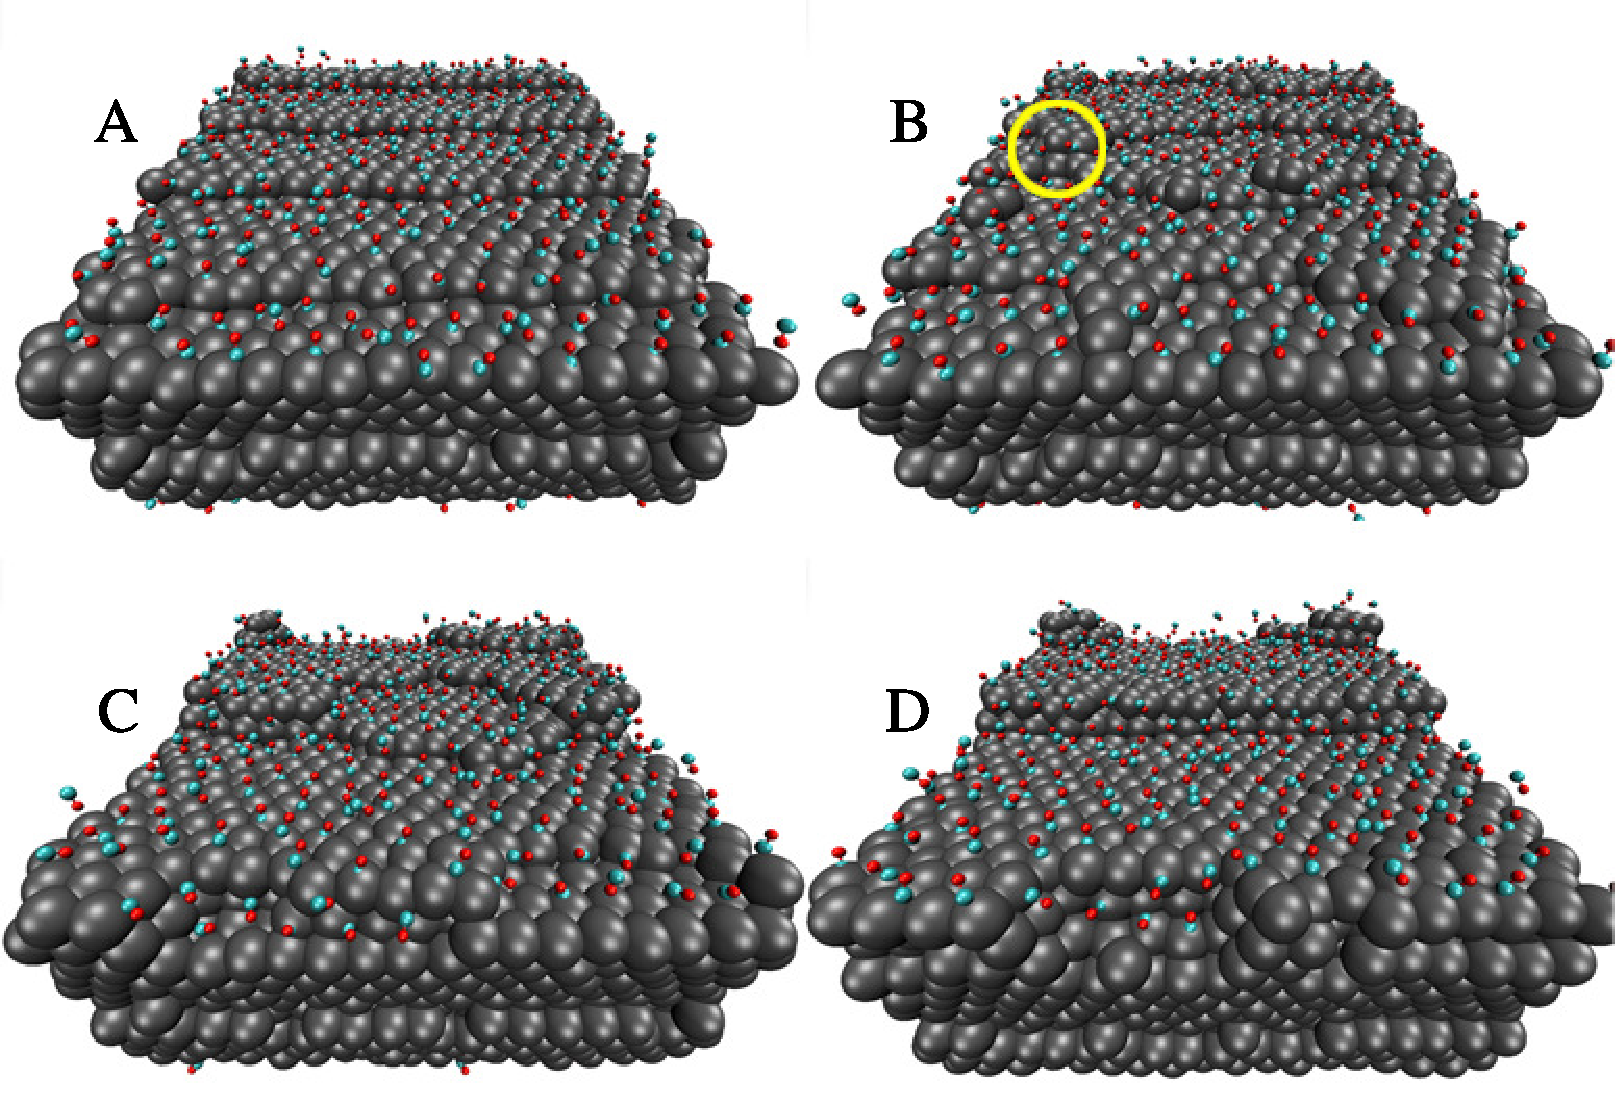
\includegraphics[width=\linewidth]{../figures/chap2/doubleLayer.pdf}
\caption{The Pt(557) / 50\% CO interface upon exposure to the CO: (a)
  258~ps, (b) 19~ns, (c) 31.2~ns, and (d) 86.1~ns after
  exposure. Disruption of the (557) step-edges occurs quickly.  The
  doubling of the layers appears only after two adjacent step-edges
  touch.  The circled spot in (b) nucleated the growth of the double
  step observed in the later configurations.}
  \label{fig:reconstruct}
\end{figure}

\subsection{Dynamics}
Previous experimental work by Pearl and Sibener\citep{Pearl}, using
STM, has been able to capture the coalescence of steps on Ni(977). The
time scale of the image acquisition, $\sim$70~s/image, provides an
upper bound for the time required for the doubling to occur. By
utilizing Molecular Dynamics we are able to probe the dynamics of
these reconstructions at elevated temperatures and in this section we
provide data on the timescales for transport properties,
e.g. diffusion and layer formation time.


\subsubsection{Transport of surface metal atoms}
%forcedSystems/stepSeparation

The wandering of a step-edge is a cooperative effect arising from the
individual movements of the atoms making up the steps. An ideal metal
surface displaying a low index facet, (111) or (100), is unlikely to
experience much surface diffusion because of the large energetic
barrier that must be overcome to lift an atom out of the surface. The
presence of step-edges and other surface features on higher-index
facets provides a lower energy source for mobile metal atoms.  Using
our potential model, single-atom break-away from a step-edge on a
clean surface still imposes an energetic penalty around
$\sim$~45~kcal/mol, but this is certainly easier than lifting the same
metal atom vertically out of the surface, \textgreater~60~kcal/mol.
The penalty lowers significantly when CO is present in sufficient
quantities on the surface. For certain distributions of CO, the
energetic penalty can fall to as low as $\sim$~20~kcal/mol. The
configurations that create these lower barriers are detailed in the
discussion section below.

Once an adatom exists on the surface, the barrier for diffusion is
negligible (\textless~4~kcal/mol for a Pt adatom). These adatoms are
then able to explore the terrace before rejoining either their
original step-edge or becoming a part of a different edge. It is an
energetically unfavorable process with a high barrier for an atom to
traverse to a separate terrace although the presence of CO can lower
the energy barrier required to lift or lower an adatom. By tracking
the mobility of individual metal atoms on the Pt and Au surfaces we
were able to determine the relative diffusion constants, as well as
how varying coverages of CO affect the diffusion. Close observation of
the mobile metal atoms showed that they were typically in equilibrium
with the step-edges.  At times, their motion was concerted, and two or
more adatoms would be observed moving together across the surfaces.

A particle was considered ``mobile'' once it had traveled more than
2~\AA~ between saved configurations of the system (typically 10-100
ps). A mobile atom would typically travel much greater distances than
this, but the 2~\AA~cutoff was used to prevent swamping the diffusion
data with the in-place vibrational movement of buried atoms. Diffusion
on a surface is strongly affected by local structures and the presence
of single and double layer step-edges causes the diffusion parallel to
the step-edges to be larger than the diffusion perpendicular to these
edges. Parallel and perpendicular diffusion constants are shown in
Figure \ref{fig:diff}.  Diffusion parallel to the step-edge is higher
than diffusion perpendicular to the edge because of the lower energy
barrier associated with sliding along an edge compared to breaking
away to form an isolated adatom.

%Diffusion graph
\begin{figure}[p!]
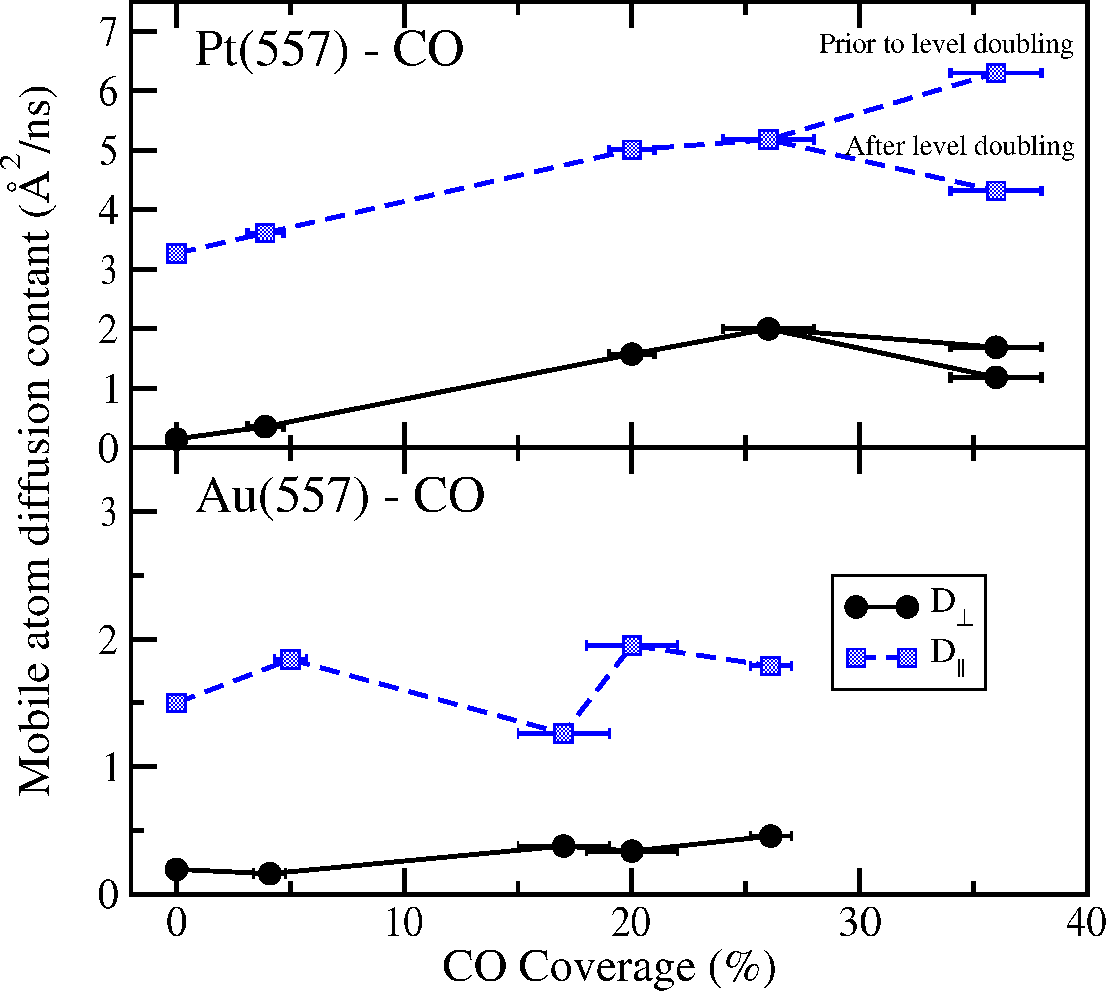
\includegraphics[width=\linewidth]{../figures/chap2/diffusion.pdf}
\caption{Diffusion constants for mobile surface atoms along directions
  parallel ($\mathbf{D}_{\parallel}$) and perpendicular
  ($\mathbf{D}_{\perp}$) to the (557) step-edges as a function of CO
  surface coverage.  The two reported diffusion constants for the 50\%
  Pt system correspond to a 20~ns period before the formation of the
  double layer (upper points), and to the full 40~ns sampling period
  (lower points).}
\label{fig:diff}
\end{figure}

The weaker Au-CO interaction is evident in the weak CO-coverage 
dependance of Au diffusion. This weak interaction leads to lower 
observed coverages when compared to dosage amounts. This further 
limits the effect the CO can have on surface diffusion. The correlation 
between coverage and Pt diffusion rates shows a near linear relationship 
at the earliest times in the simulations. Following double layer formation, 
however, there is a precipitous drop in adatom diffusion. As the double 
layer forms, many atoms that had been tracked for mobility data have 
now been buried, resulting in a smaller reported diffusion constant. A
secondary effect of higher coverages is CO-CO cross interactions that
lower the effective mobility of the Pt adatoms that are bound to each CO.
This effect would become evident only at higher coverages. A detailed
account of Pt adatom energetics follows in the Discussion.
 
\subsubsection{Dynamics of double layer formation}
The increased diffusion on Pt at the higher CO coverages is the primary 
contributor to double layer formation. However, this is not a complete 
explanation -- the 33\%~Pt system has higher diffusion constants, but 
did not show any signs of edge doubling in 40~ns. On the 50\%~Pt 
system, one double layer formed within the first 40~ns of simulation time, 
while two more were formed as the system was allowed to run for an 
additional 110~ns (150~ns total). This suggests that this reconstruction 
is a rapid process and that the previously mentioned upper bound is a 
very large overestimate.\citep{Williams:1991,Pearl} In this system the first 
appearance of a double layer appears at 19~ns into the simulation. 
Within 12~ns of this nucleation event, nearly half of the step has formed 
the double layer and by 86~ns the complete layer has flattened out. 
From the appearance of the first nucleation event to the first observed 
double layer, the process took $\sim$20~ns. Another $\sim$40~ns was 
necessary for the layer to completely straighten. The other two layers in 
this simulation formed over periods of 22~ns and 42~ns respectively. 
A possible explanation for this rapid reconstruction is the elevated 
temperatures under which our systems were simulated. The process 
would almost certainly take longer at lower temperatures. Additionally, 
our measured times for completion of the doubling after the appearance 
of a nucleation site are likely affected by our periodic boxes. A longer 
step-edge will likely take longer to ``zipper''. 


%Discussion
\section{Discussion}
We have shown that a classical potential is able to model the initial
reconstruction of the Pt(557) surface upon CO adsorption, and have
reproduced the double layer structure observed by Tao {\it et
  al}.\citep{Tao:2010}. Additionally, this reconstruction appears to be
rapid -- occurring within 100 ns of the initial exposure to CO.  Here
we discuss the features of the classical potential that are
contributing to the stability and speed of the Pt(557) reconstruction.

\subsection{Diffusion}
The perpendicular diffusion constant appears to be the most important
indicator of double layer formation. As highlighted in Figure
\ref{fig:reconstruct}, the formation of the double layer did not begin
until a nucleation site appeared.  Williams {\it et
  al}.\citep{Williams:1991,Williams:1994} cite an effective edge-edge
repulsion arising from the inability of edge crossing.  This repulsion
must be overcome to allow step coalescence.  A larger
$\textbf{D}_\perp$ value implies more step-wandering and a larger
chance for the stochastic meeting of two edges to create a nucleation
point.  Diffusion parallel to the step-edge can help ``zipper'' up a
nascent double layer. This helps explain the rapid time scale for
double layer completion after the appearance of a nucleation site, while
the initial appearance of the nucleation site was unpredictable.

\subsection{Mechanism for restructuring}
Since the Au surface showed no large scale restructuring in any of our
simulations, our discussion will focus on the 50\% Pt-CO system which
did exhibit doubling. A number of possible mechanisms exist to explain
the role of adsorbed CO in restructuring the Pt surface. Quadrupolar
repulsion between adjacent CO molecules adsorbed on the surface is one
possibility.  However, the quadrupole-quadrupole interaction is
short-ranged and is attractive for some orientations.  If the CO
molecules are ``locked'' in a vertical orientation, through atop
adsorption for example, this explanation would gain credence. Within
the framework of our classical potential, the calculated energetic
repulsion between two CO molecules located a distance of
2.77~\AA~apart (nearest-neighbor distance of Pt) and both in a
vertical orientation, is 8.62 kcal/mol. Moving the CO to the second
nearest-neighbor distance of 4.8~\AA~drops the repulsion to nearly
0. Allowing the CO to rotate away from a purely vertical orientation
also lowers the repulsion. When the carbons are locked at a distance
of 2.77~\AA, a minimum of 6.2 kcal/mol is reached when the angle
between the 2 CO is $\sim$24\textsuperscript{o}.  The calculated
barrier for surface diffusion of a Pt adatom is only 4 kcal/mol, so
repulsion between adjacent CO molecules bound to Pt could indeed
increase the surface diffusion. However, the residence time of CO on
Pt suggests that the CO molecules are extremely mobile, with diffusion
constants 40 to 2500 times larger than surface Pt atoms. This mobility
suggests that the CO molecules jump between different Pt atoms
throughout the simulation.  However, they do stay bound to individual
Pt atoms for long enough to modify the local energy landscape for the
mobile adatoms.

A different interpretation of the above mechanism which takes the
large mobility of the CO into account, would be in the destabilization
of Pt-Pt interactions due to bound CO.  Destabilizing Pt-Pt bonds at
the edges could lead to increased step-edge breakup and diffusion. On
the bare Pt(557) surface the barrier to completely detach an edge atom
is $\sim$43~kcal/mol, as is shown in configuration (a) in Figures
\ref{fig:SketchGraphic} \& \ref{fig:SketchEnergies}. For certain
configurations, cases (e), (g), and (h), the barrier can be lowered to
$\sim$23~kcal/mol by the presence of bound CO molecules. In these
instances, it becomes energetically favorable to roughen the edge by
introducing a small separation of 0.5 to 1.0~\AA. This roughening
becomes immediately obvious in simulations with significant CO
populations. The roughening is present to a lesser extent on surfaces
with lower CO coverage (and even on the bare surfaces), although in
these cases it is likely due to random fluctuations that squeeze out
step-edge atoms. Step-edge breakup by direct single-atom translations
(as suggested by these energy curves) is probably a worst-case
scenario.  Multistep mechanisms in which an adatom moves laterally on
the surface after being ejected would be more energetically favorable.
This would leave the adatom alongside the ledge, providing it with
five nearest neighbors.  While fewer than the seven neighbors it had
as part of the step-edge, it keeps more Pt neighbors than the three
neighbors an isolated adatom has on the terrace. In this proposed
mechanism, the CO quadrupolar repulsion still plays a role in the
initial roughening of the step-edge, but not in any long-term bonds
with individual Pt atoms.  Higher CO coverages create more
opportunities for the crowded CO configurations shown in Figure
\ref{fig:SketchGraphic}, and this is likely to cause an increased
propensity for step-edge breakup.

%Sketch graphic of different configurations
\begin{figure}[p!]
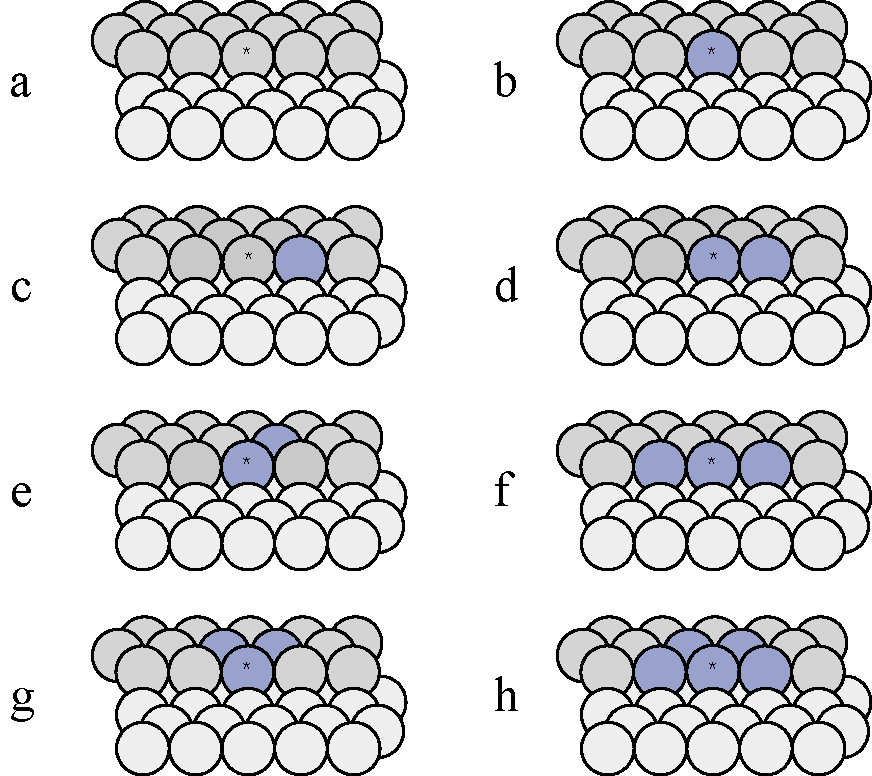
\includegraphics[width=\linewidth]{../figures/chap2/COpaths.pdf}
\caption{Configurations used to investigate the mechanism of step-edge
  breakup on Pt(557). In each case, the central (starred) atom was
  pulled directly across the surface away from the step edge.  The Pt
  atoms on the upper terrace are colored dark grey, while those on the
  lower terrace are in white.  In each of these configurations, some
  of the atoms (highlighted in blue) had CO molecules bound in the
  vertical atop position.  The energies of these configurations as a
  function of central atom displacement are displayed in Figure
  \ref{fig:SketchEnergies}.}
\label{fig:SketchGraphic}
\end{figure}

%energy graph corresponding to sketch graphic
\begin{figure}[p!]
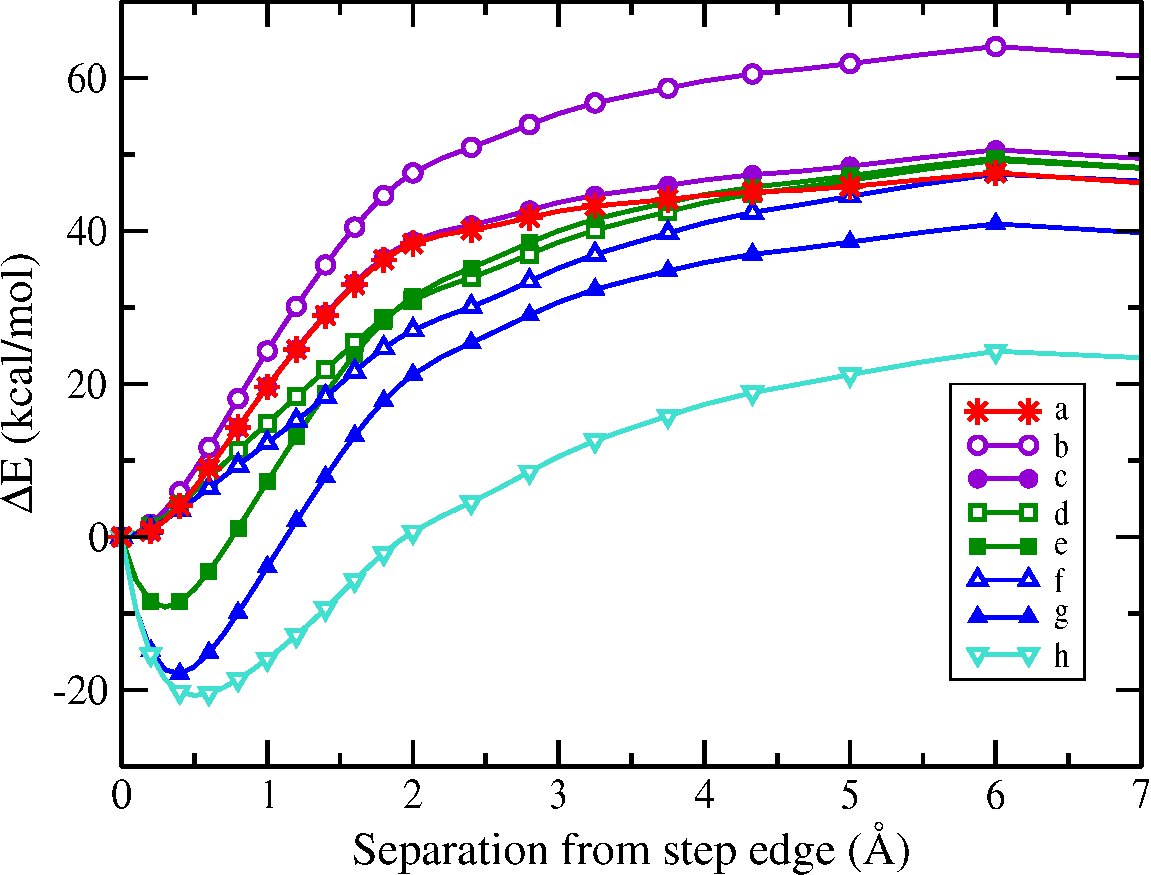
\includegraphics[width=\linewidth]{../figures/chap2/separation.pdf}
\caption{Energies for displacing a single edge atom perpendicular to
  the step edge as a function of atomic displacement. Each of the
  energy curves corresponds to one of the labeled configurations in
  Figure \ref{fig:SketchGraphic}, and the energies are referenced to
  the unperturbed step-edge.  Certain arrangements of bound CO
  (notably configurations g and h) can lower the energetic barrier for
  creating an adatom relative to the bare surface (configuration a).}
\label{fig:SketchEnergies}
\end{figure}

While configurations of CO on the surface are able to increase
diffusion and the likelihood of edge wandering, this does not provide
a complete explanation for the formation of double layers. If adatoms
were constrained to their original terraces then doubling could not
occur.  A mechanism for vertical displacement of adatoms at the
step-edge is required to explain the doubling.

We have discovered one possible mechanism for a CO-mediated vertical
displacement of Pt atoms at the step edge. Figure \ref{fig:lambda}
shows four points along a reaction coordinate in which a CO-bound
adatom along the step-edge ``burrows'' into the edge and displaces the
original edge atom onto the higher terrace.  A number of events
similar to this mechanism were observed during the simulations.  We
predict an energetic barrier of 20~kcal/mol for this process (in which
the displaced edge atom follows a curvilinear path into an adjacent
3-fold hollow site).  The barrier heights we obtain for this reaction
coordinate are approximate because the exact path is unknown, but the
calculated energy barriers would be easily accessible at operating
conditions.  Additionally, this mechanism is exothermic, with a final
energy 15~kcal/mol below the original $\lambda = 0$ configuration.
When CO is not present and this reaction coordinate is followed, the
process is endothermic by 3~kcal/mol.  The difference in the relative
energies for the $\lambda=0$ and $\lambda=1$ case when CO is present
provides strong support for CO-mediated Pt-Pt interactions giving rise
to the doubling reconstruction.

%lambda progression of Pt -> shoving its way into the step
\begin{figure}[p!]
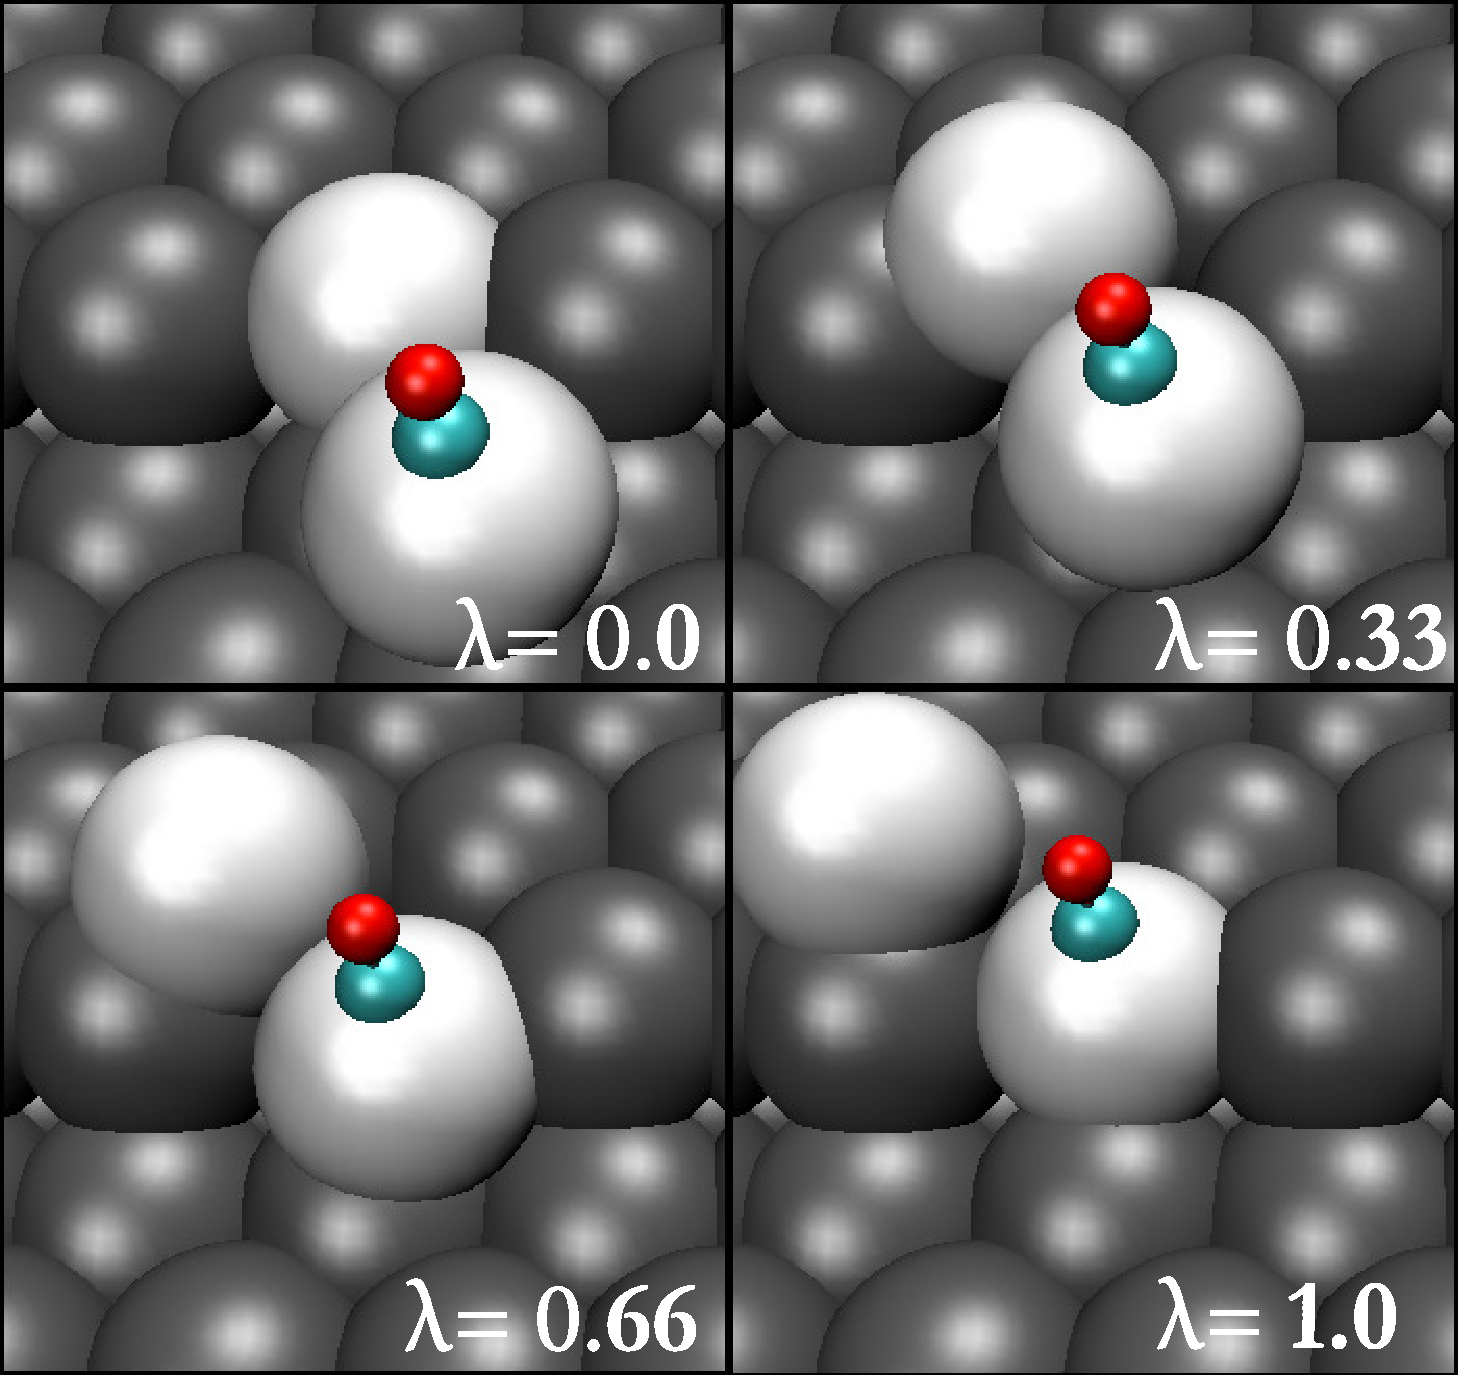
\includegraphics[width=\linewidth]{../figures/chap2/rxn.pdf}
\caption{Points along a possible reaction coordinate for CO-mediated
  edge doubling. Here, a CO-bound adatom burrows into an established
  step edge and displaces an edge atom onto the upper terrace along a
  curvilinear path.  The approximate barrier for the process is
  20~kcal/mol, and the complete process is exothermic by 15~kcal/mol
  in the presence of CO, but is endothermic by 3~kcal/mol without CO.}
\label{fig:lambda}
\end{figure}

The mechanism for doubling on the Pt(557) surface appears to require
the cooperation of at least two distinct processes. For complete
doubling of a layer to occur there must be a breakup of one
terrace. These atoms must then ``disappear'' from that terrace, either
by travelling to the terraces above or below their original levels.
The presence of CO helps explain mechanisms for both of these
situations. There must be sufficient breakage of the step-edge to
increase the concentration of adatoms on the surface and these adatoms
must then undergo the burrowing highlighted above (or a comparable
mechanism) to create the double layer.  With sufficient time, these
mechanisms working in concert lead to the formation of a double layer.

\subsection{CO Removal and double layer stability}
Once the double layers had formed on the 50\%~Pt system, they remained
stable for the rest of the simulation time with minimal movement.
Random fluctuations that involved small clusters or divots were
observed, but these features typically healed within a few
nanoseconds.  Within our simulations, the formation of the double
layer appeared to be irreversible and a double layer was never
observed to split back into two single layer step-edges while CO was
present.

To further gauge the effect CO has on this surface, additional
simulations were run starting from a late configuration of the 50\%~Pt
system that had already formed double layers. These simulations then
had their CO molecules suddenly removed.  The double layer broke apart
rapidly in these simulations, showing a well-defined edge-splitting
after 100~ps. Configurations of this system are shown in Figure
\ref{fig:breaking}. The coloring of the top and bottom layers helps to
show how much mixing the edges experience as they split. These systems
were only examined for 10~ns, and within that time despite the initial
rapid splitting, the edges only moved another few \AA~apart. It is
possible that with longer simulation times, the (557) surface recovery
observed by Tao {\it et al}.\citep{Tao:2010} could also be recovered.

%breaking of the double layer upon removal of CO
\begin{figure}[p!]
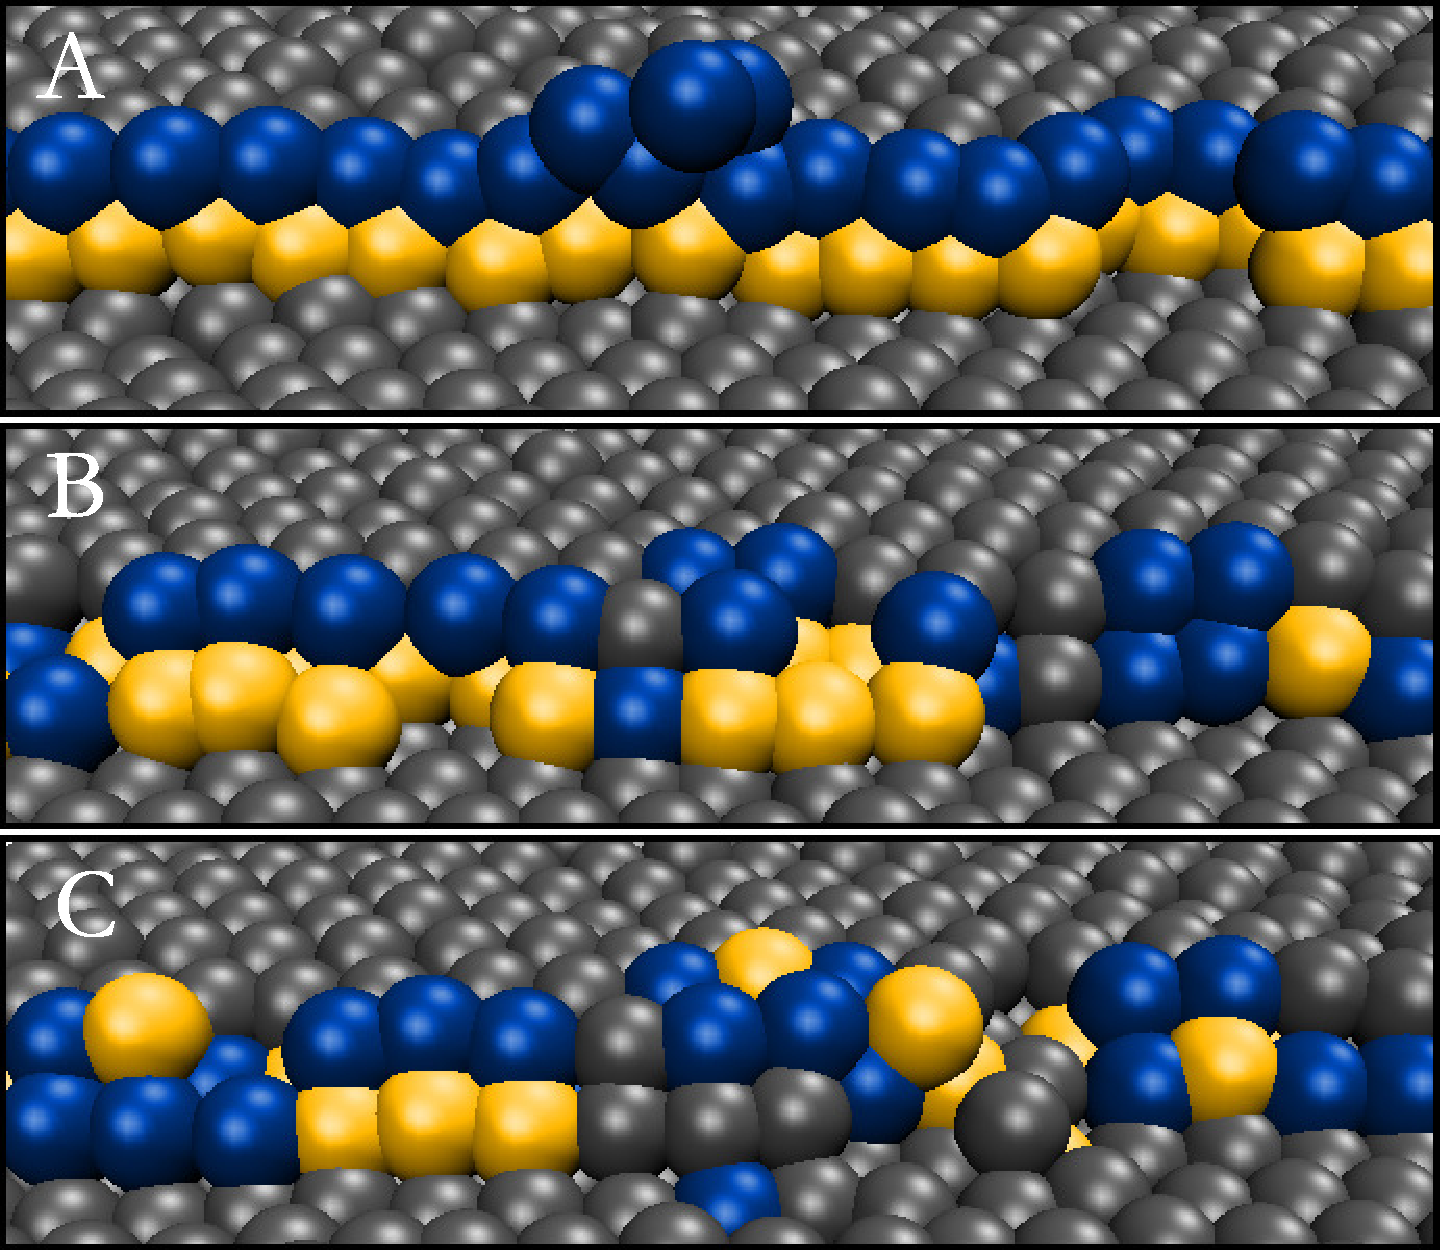
\includegraphics[width=\linewidth]{../figures/chap2/layerBreaking.pdf}
\caption{Behavior of an established (111) double step after removal of
  the adsorbed CO: (A) 0~ps, (B) 100~ps, and (C) 1~ns after the
  removal of CO.  Nearly immediately after the CO is removed, the
  step edge reforms in a (100) configuration, which is also the step
  type seen on clean (557) surfaces. The step separation involves
  significant mixing of the lower and upper atoms at the edge.}
\label{fig:breaking}
\end{figure}


%Peaks!
%\begin{figure}[H]
%\includegraphics[width=\linewidth]{doublePeaks_noCO.png}
%\caption{At the initial formation of this double layer  ( $\sim$ 37 ns) there is a degree
 %of roughness inherent to the edge. The next $\sim$ 40 ns show the edge with 
 %aspects of waviness and by 80 ns the double layer is completely formed and smooth. }
%\label{fig:peaks}
%\end{figure}


%Don't think I need this
%clean surface...
%\begin{figure}[H]
%\includegraphics[width=\linewidth]{557_300K_cleanPDF}
%\caption{}

%\end{figure}
%\label{fig:clean}


\section{Conclusion}
The strength and directionality of the Pt-CO binding interaction, as
well as the large quadrupolar repulsion between atop-bound CO
molecules, help to explain the observed increase in surface mobility
of Pt(557) and the resultant reconstruction into a double-layer
configuration at the highest simulated CO-coverages.  The weaker Au-CO
interaction results in significantly lower adataom diffusion
constants, less step-wandering, and a lack of the double layer
reconstruction on the Au(557) surface.

An in-depth examination of the energetics shows the important role CO
plays in increasing step-breakup and in facilitating edge traversal
which are both necessary for double layer formation.

%Things I am not ready to remove yet

%Table of Diffusion Constants
%Add gold?M
% \begin{table}[H]
%   \caption{}
%   \centering
% \begin{tabular}{| c | cc | cc | }
%   \hline
%   &\multicolumn{2}{c|}{\textbf{Platinum}}&\multicolumn{2}{c|}{\textbf{Gold}} \\
%   \hline
%   \textbf{Surface Coverage} & $\mathbf{D}_{\parallel}$ & $\mathbf{D}_{\perp}$ & $\mathbf{D}_{\parallel}$ & $\mathbf{D}_{\perp}$  \\
%   \hline
%   50\% & 4.32(2) & 1.185(8)  & 1.72(2) & 0.455(6) \\
%   33\% & 5.18(3)  & 1.999(5)  & 1.95(2) & 0.337(4)   \\
%   25\% & 5.01(2)  & 1.574(4)  & 1.26(3) & 0.377(6) \\
%   5\%   & 3.61(2)  & 0.355(2)  & 1.84(3)  & 0.169(4)  \\
%   0\%   & 3.27(2)  & 0.147(4)  & 1.50(2)  & 0.194(2)   \\
%   \hline 
% \end{tabular}
% \end{table}




\chapter{CARBON MONOXIDE-INDUCED ISLAND FORMATION ON PT/PD(557) SURFACE ALLOYS}
\label{chap:island}


%\begin{abstract}
%  Stepped surfaces of bimetallic \ce{Pd}/\ce{Pt} alloys were exposed
%  to a range of coverages of adsorbed carbon monoxide (\ce{CO}) using
%  molecular dynamics (MD) simulations. Metal-\ce{CO} interactions for
%  both metals were parameterized from experimental data and Density
%  Functional Theory (DFT) calculations, providing classical potentials
%  that capture the atop binding preference on \ce{Pt} and the
%  hollow/bridge preference on \ce{Pd}.  The MD simulations indicate
%  significant restructuring in the surface alloy, with \ce{Pt}-rich
%  islands forming on the \ce{Pd} substrate within 60~ns.  The
%  time-dependence of the surface domain sizes and the dynamics of
%  nearest-neighbor metal populations suggest that multi-layer \ce{Pt}
%  islands form more rapidly in the presence of adsorbed \ce{CO}.  We
%  find that the different binding preference of \ce{CO} adsorbed to
%  the two metals can help explain the observed stabilization of the
%  \ce{Pd} surface structures as well as the roughening of the \ce{Pt}
%  step edges.  Because the \ce{CO} acts to lower the surface energy of
%  the \ce{Pt}, we conclude that the mechanism for accelerating
%  \ce{Pt}-island formation is kinetic in nature.
%\end{abstract}


In this chapter we explore a bimetallic \ce{Pt/Pd} near surface alloy (NSA)
exposed to \ce{CO} through molecular dynamics simulations. A forcefield
describing the \ce{Pd\bond{-}CO} was parameterized as a part of this work and
a pure \ce{Pd} (557) system was modeled as a control. The differing binding
characteristics of \ce{CO}, site and strength, on the two metals was
hypothesized to lead to significant exposure of the underlying \ce{Pd}
requiring the overlayer of \ce{Pt} to either bury itself or cluster into small
nanostructures on the surface. The stability of the systems and specifically
the \ce{Pt} overlayer was examined as a function of time and \ce{CO} coverage.
Ultimately the binding preference of the \ce{CO} was discovered to play a
primary role in describing the preferred equilibrium states of these systems.


%\section{Introduction}

%Materials based on metallic \ce{Pt} and \ce{Pd} are important
%catalysts for the oxygen reduction
%(ORR)\citep{Lim:2009fk, Liu:2012bs, Limpattayanate:2014ij} and oxygen
%evolution reactions (OER).\citep{Stamenkovic:2007kk, Reier:2012uq} These
%reactions are important in proton-exchange membrane (PEM) fuel
%cells,\citep{Bliznakov:2012kx, Shao:2013rm} as well as in the charging
%and discharging of \ce{Li}-air batteries.\citep{Lu:2011vn}
%Oxide-supported noble metal nanoparticles also play an important role in
%the water-gas shift reaction.\citep{Bunluesin:1998ys, Kugai:2011rt}
%
%However, the expense of \ce{Pt} metal coupled to the slow kinetics of
%the ORR on pure \ce{Pt} or \ce{Pt}/\ce{C} systems remain barriers to
%large-scale implementation of fuel cells. Strategies involving
%bimetallic particles, surface alloys, and core-shell nanostructures
%are currently under investigation in hopes of eliminating these
%barriers.\citep{Gao:2009oj, Gao:2009wo, Kim:2013mi} The coupling of two
%(or more) components in these structures allows for a large accesible
%design space for various catalytic properties, whether that be
%catalytic activity,\citep{Kim:2013mi, Sneed:2014fj, Gu:2015cr} thermal
%stability,\citep{Cao:2010gf, Yang:0pd, Huang:2012ul} or resistance to
%deactivation.\citep{Yu:2013fr, Zhang:2015yq} Specifically,
%\ce{Pt\bond{-}Pd} nanoparticles have been shown to have increased
%activity for the ORR reaction,\citep{Lim:2009fk, Liu:2012bs, Shao:2013rm}
%while \ce{Pt\bond{-}Au} nanoparticles were reported as being more
%stable over repeated potential cycling.\citep{Zhang:2007uq}
%
%Bimetallic \ce{Pt}/\ce{Pd} mixtures also find widespread use in diesel
%oxidation catalysts (DOC) which complete the oxidation of carbon
%monoxide and partially-combusted hydrocarbons, and reduce the nitrogen
%oxides in combustion gases.\citep{Morlang:2005uq, Russell:2011fk}
%\ce{Pd} is a particularly useful metal for diesel catalysts because it
%has a lower intrinsic \ce{SO2} oxidation activity than
%\ce{Pt}.\citep{Russell:2011fk} The \ce{Pt}/\ce{Pd} bimetallic catalyst
%also significantly inhibits sintering of the particles at higher
%temperatures, relative to pure \ce{Pt} catalysts.\citep{Morlang:2005uq}
%
%Catalytic activity is dependent on the exposed structure of \ce{Pt} in
%many of these applications. Reconstruction of the exposed \ce{Pt} can
%therefore change the effectiveness of a given \ce{Pt}-\ce{M} species.
%Of particular interest in diesel oxidation catalysis is carbon
%monoxide (\ce{CO}) and its strong binding affinity for \ce{Pt} and
%\ce{Pd}. Tao \textit{et al.} have shown that the presence of \ce{CO}
%can induce reversible surface reconstructions on a stepped
%\ce{Pt}(557) surface.\citep{Tao:2010aa} Significant experimental and
%theoretical work has been done to more fully characterize the effect
%adsorbed \ce{CO} has on
%\ce{Pt}.\citep{Batteas:1996rc, Thostrup:2001dn, McCarthy:2012qd, Michalka:2013aa, Carenco:2014aa}
%
%This paper describes an investigation into the effects of carbon
%monoxide adsorption on surface restructuring of pure \ce{Pd}(557) and
%\ce{Pt}/\ce{Pd}(557) surface alloys using molecular dynamics
%simulations. Since the long-time dynamics of the restructuring process
%are of particular interest, classical force fields which balance
%computational efficiency against chemical accuracy were employed.

\section{Methodology}
\subsection{Interaction potentials}

%Modeling large metallic interfaces (10\textsuperscript{3}-
%10\textsuperscript{4} atoms) over relatively long time scales (10-100
%ns) requires the use of empirical potentials. Cohesive and surface
%energies in metals are not reproduced with purely pairwise
%interactions, so a number of empirical potentials have been developed
%for modeling transition metals.  These include the embedded atom
%method (EAM)\citep{Foiles:1986ky}, Finnis-Sinclair,\citep{Finnis:1984hl} and
%Sutton-Chen-based models like QSC.\citep{Goddard:1998qsc} These models describe an
%atom as a positively charged core with a radially-decaying valence
%electron density.  Refinements include angle dependent EAM
%implementations,\citep{Baskes:1987aa} that treat BCC metals more
%accurately.
%
%In EAM, the energy for embedding a metallic atom $i$ at a specific
%location in the system requires the electron density at that location,
%\begin{equation*}
%\rho_i = \sum_{j\neq i} \rho_j(r_{ij}).
%\end{equation*}
%This density at site $i$, $\rho_i$ depends on the contributions to the
%electron density from all other atoms in the system.  Here,
%$\rho_j(r)$ describes the distance dependence of the valence electron
%distribution of atom $j$.  Atom $i$'s contribution to the potential
%energy can then be obtained from an embedding functional, $F_i\left[
%  \rho_i \right]$, that depends on $\rho_i$, as well as from a sum of
%pairwise interactions,
%\begin{equation*}
%  V_i =  F[ \rho_i ]  + \sum_{j \neq i} \phi_{ij}(r_{ij})
%\end{equation*}
%
%The embedding energy functional is parameterized for each metallic
%atom type, and depends only on the local electron density, $\rho_i$.
%Thus, the cohesive energy for atom $i$ depends on collective
%contributions from all of the surrounding metal atoms, and is an
%explicitly non-pairwise additive quantity.
As in Chapter \ref{chap:PtAu}, the Embedded-Atom-Method (EAM) was used to model
the metal-metal interactions while the Karplus and Straub model of carbon
monoxide was used to describe the \ce{CO} self interactions. Due to its development, the EAM
method is effective at modeling alloys as the density portion is unchanged
and only the short-ranged repulsions, $\phi$, need to be modified. EAM treats
short-range repulsions as a pairwise contribution that models the repulsive
overlap of the positively-charged cores. For alloys, mixing rules as outlined
by Johnson \citep{Johnson:1989yr} were used to compute the heterogeneous pair
potential,

\begin{equation*} 
\phi_{ab}(r) = \frac{1}{2}
\bigg\{ \bigg(
\frac{\rho_b(r)}{\rho_a(r)}
\bigg) \phi_{aa}(r)
+ \bigg(
\frac{\rho_a(r)}{\rho_b(r)}
\bigg)\phi_{bb}(r) 
\bigg\}
\end{equation*} 

In this work, we have employed the embedded atom method (EAM) to describe the
\ce{Pt} and \ce{Pd} electron densities, embedding functionals, and pair
potentials,\citep{Foiles:1986ky} utilizing the Johnson mixing rules for the
\ce{Pt\bond{-}Pd} cross-interactions.\citep{Johnson:1989yr}

The \ce{Pt\bond{-}CO} interactions have been modified from 
fits in Chapter \ref{chap:PtAu} to account for recently-published DFT
data.\citep{Deshlahra:2012aa} This modification yields a slightly weaker
\ce{Pt\bond{-}CO} binding energy, but maintains the atop site
preference.  The potential energy for the interaction of one \ce{CO}
molecule with one metal atom,
\begin{equation*}
V_\mathrm{M\mhyphen CO} = 4 \epsilon \left(
  \left(\frac{\sigma}{r_\mathrm{M\mhyphen C}}\right)^{12} -
  \left(\frac{\sigma}{r_\mathrm{M\mhyphen C}}\right)^6 \right) +
D e^{-2 \gamma (r_\mathrm{M\mhyphen O} - r_e)}
\label{eq:pot}
\end{equation*}
is modeled using a Lennard-Jones interaction between the metal atom
(M) and the carbon along with a repulsive Morse potential between the
metal atom and the oxygen.

Both the \ce{Pd\bond{-}CO} and \ce{Pt\bond{-}CO} interaction
potentials were parameterized as part of this work. The basic model,
using a full Morse potential between the metal and oxygen site and a
Lennard-Jones interaction between the metal and the carbon site, was
introduced by Korzeniewski \textit{et al.}\citep{Korzeniewski:1986kl} One key
difference from the potential in Refs.\citep{Korzeniewski:1986kl} and our
earlier fits in Refs.\citep{Michalka:2013aa} is that the
\ce{M\bond{-}O} bond is modeled here using a purely repulsive Morse
potential. The parameters were fit to reflect binding energies and
binding site preferences on the \ce{M}(111) surfaces.  The functional
forms and the broad repulsive \ce{M\bond{-}O} contribution are
flexible enough to reproduce the atop preference for \ce{Pt\bond{-}CO}
as well as the bridge/hollow preference for \ce{Pd\bond{-}CO}.
Parameters for the potentials are given in
Table~\ref{tab:CO_parameters} and the calculated binding energies at
various binding sites are shown in Table~\ref{tab:CO_energies}.

\begin{table} 
\caption{PARAMETERS FOR THE PT-CO AND PD-CO INTERACTIONS}
%\caption{Parameters for the M-\ce{CO} cross-interactions. Metal-Carbon
%  interactions are modeled with Lennard-Jones potentials, while the
%  metal-Oxygen interactions are fit using repulsive Morse potentials.
%  Distances are given in \AA~and energies in
%  kcal/mol.\label{tab:CO_parameters}}
\centering
\begin{threeparttable}  
\centering
\begin{tabular}{ c  cc  c  ccc }
\hline
\hline
 &  $\sigma$\tnote{a} & $\epsilon$\tnote{b} & & $r$\tnote{a} & $D$\tnote{b} & $\gamma$ (\AA$^{-1}$) \\
\midrule
\textbf{\ce{Pt\bond{-}C}} & 1.41 & 45  & \textbf{\ce{Pt\bond{-}O}} & 4.4  & 0.05 & 1.8 \\
\textbf{\ce{Pd\bond{-}C}} & 1.6 &  40  & \textbf{\ce{Pd\bond{-}O}} & 4.95 & 0.05 & 1.45\\
\hline
\hline
\end{tabular}
\begin{tablenotes}
  \item Metal-C interactions are modeled with Lennard-Jones potentials, while the metal-O interactions were fit to Morse potentials.
  \item[a] Distances are given in \AA
  \item[b] Energies are given in kcal/mol
\end{tablenotes}
\end{threeparttable}
\label{tab:CO_parameters}
\end{table}

%Table of energies
\begin{table}
  \caption{ADSORPTION ENERGIES FOR A CO MOLECULE AT THE THREE PRIMARY BINDING SITES ON M(111)}
%  \caption{Single-site adsorption energies for a \ce{CO} molecule at
%    the three binding sites on \ce{M}(111) using the potentials
%    described in Table \ref{tab:CO_parameters}.  These values are
%    compared with 
%    electronic structure and experimental desorption
%    data when available. Note that the electronic structure values are
%    for surface 
%    coverages of $\ge$ 0.25 ML, and
%    experimental values are (in most cases) extrapolated to zero
%    coverage from desorption energies at higher coverages.  All values
%    are in eV.}
\centering
\begin{threeparttable}
\begin{tabular}{ c  ccc  c }
  \hline
  \hline
  & Site & This Model\tnote{a} & DFT\tnote{a} & Experimental\tnote{a} \\
  \hline
  \textbf{\ce{Pt\bond{-}CO}} & atop   & -1.47 & -1.48\citep{Deshlahra:2012aa} & -1.39\citep{Kelemen:1979ad}, -1.43\citep{Ertl:1977cg}, -1.90\citep{Yeo:1997th} \\
                 & bridge & -1.13 & -1.47\citep{Deshlahra:2012aa} &  \\
                 & hollow & -1.02 & -1.45\citep{Deshlahra:2012aa} &  \\
\hline
  \textbf{\ce{Pd\bond{-}CO}} & atop   & -1.54 & -1.44\citep{Honkala:2001sf} &  \\
                 & bridge & -1.65 & -1.83\citep{Honkala:2001sf} &  \\
                 & hollow & -1.60 & -1.99\citep{Honkala:2001sf} & -1.30\citep{Szanyi:1992aa}, -1.47\citep{Ertl:1970aa}, -1.54\citep{Guo:1989aa} \\
  \hline
  \hline
\end{tabular}
\begin{tablenotes}
  \item The energies are obtained using the potentials described in Table \ref{tab:CO_parameters}. These values are compared with electronic structure and experimental desorption data when available Note that the electronic structure values are for surface coverages of $\ge$ 0.25 ML, and experimental values are (in most cases) extrapolated to zero coverage from desorption energies at higher coverages.
  \item[a] All values are in eV
\end{tablenotes}
\end{threeparttable}
\label{tab:CO_energies}
\end{table}
This \ce{Pd\bond{-}CO} model does not have a strong preference for
either the bridge or hollow binding sites, so it may overestimate the
bridge-site binding at low coverages, but at higher coverages, the
experimental situation is somewhat less clear.\citep{Wong:1991ta}
Studies using low-energy electron diffraction (LEED) and
\ce{C\bond{-}O} stretching frequencies of \ce{CO} bound to
\ce{Pd}(111) suggest that the 3-fold hollow sites are preferred at low
coverages,\citep{Bradshaw:1978uf, Conrad:1978fx, Ohtani:1987zh} where it
forms a $(\sqrt{3} \times \sqrt{3}) R~30^{\circ}$ pattern.  These
observations are supported by temperature desorption
spectroscopy,\citep{Guo:1989aa} and infrared absorption
spectroscopy~\citep{Szanyi:1992aa} where binding energies have been
reported to lie between -1.3 and -1.54 eV.

At higher \ce{CO} coverages (e.g. $> 0.5$ ML), the preferred binding
of \ce{CO} on \ce{Pd}(111) appears to be a $c(4\times2)$ ordered
structure with the \ce{CO} bound to the bridge
sites.\citep{Bradshaw:1978uf} 

Theoretical work by Honkala \textit{et al.}\citep{Honkala:2001sf} using
DFT with the generalized gradient approximation (GGA) to describe
electron exchange correlation and pseudopotentials for the \ce{Pd}
atoms also reported the FCC site as the most favorable binding
position with a binding energy of -2.00 eV compared to the bridge site
binding energy of -1.83 eV at 0.33 monolayer.

High resolution x-ray photoelectron spectroscopy (XPS) results from
Surnev \textit{et al.}\citep{Surnev:2000uk} confirm that the preferred
low coverage ($< $ 0.1 ML) binding site is the FCC hollow, but also
suggest a competition between hollow and bridge binding for coverages
between 0.1 and 0.32 ML, suggesting similar binding energies for these
two sites. Additional DFT calculations from Loffreda \textit{et
al.}\citep{Loffreda:1999vl} suggest that as the coverage increases, the
binding energy difference shrinks, as at 0.5 ML the hollow to bridge
energy difference is 0.06 eV (-1.85 hollow, -1.79 bridge).

Although the weak preference for hollow vs. bridge sites at low
coverage is not captured by the \ce{Pd\bond{-}CO} fit, at low
temperatures on \ce{Pd}(111), a 0.5 ML coverage of \ce{CO} interacting
with the potential in Table \ref{tab:CO_parameters} does produce
domains with the $c(4\times2)$ ordered structure (see 
appendix \ref{app:SI}).

Experimental work on CO on Pt(111) using LEED has suggested that the
atop binding is 70 meV stronger than the bridge
site~\citep{Schweizer:1989fk} and forms a
$(\sqrt{3} \times \sqrt{3}) R~30^{\circ}$ structure on solely atop
sites at low surface coverages.\citep{Kelemen:1979ad} Because our Pt-CO
model uses relatively long-range repulsive Morse interactions to
preserve the CO orientation on the surface, it overestimates the atop
binding preference relative to the DFT calculations.  However, the
model is able to reproduce small domains of the
$(\sqrt{3} \times \sqrt{3}) R~30^{\circ}$ structures (see 
appendix \ref{app:SI}).

\subsection{(557) Interfaces and surface alloys}
The \ce{Pd}(557) model is contained in an orthorhombic periodic box
with dimensions of $55.09 \times 49.48 \times 120$~\AA~ while the
surface alloys (\ce{Pt}(557) surface layers, with \ce{Pd} bulk) have
dimensions of $54.875 \times 49.235 \times 120$~\AA.  The \ce{Pd}
system consists of 9 layers of \ce{Pd} while our surface alloys
consist of 7 layers of \ce{Pd} sandwiched between 2 single layers of
\ce{Pt}.  Both the pure \ce{Pd} slab and the surface alloy systems are
$\sim$22~\AA~ thick. The lattice constants for \ce{Pd} and \ce{Pt},
3.89 and 3.92~\AA, respectively, result in minimal strain energy in
the alloy, and the relaxed geometries of the two interfaces are
therefore quite similar.

The systems are cut from a FCC crystal along the (557) plane, and are
rotated so that they are periodic in the $x$ and $y$ directions,
exposing (557) facets on both the positive and negative sides of the
$z$-axis of the box.

Simulations of the metal without any adsorbate present were performed
at temperatures ranging from 300 to 900~K to establish the stability
of the (557) surface without a \ce{CO} overlayer.  The bare systems
were run in the canonical (NVT) ensemble at 850~K for 200~ps and the
microcanonical (NVE) ensemble for 1~ns, and displayed minimal changes
in the (557) structure during this period.  This temperature is well
below previously simulated melting temperatures for \ce{Pt}/\ce{Pd}
alloyed nanoparticles in both free and graphite-supported
configurations.\citep{Sankaranarayanan:2005bh, Sankaranarayanan:2005qf, Fernandez:2013yg}

Ten systems were constructed, corresponding to five \ce{CO}-coverage
levels for each metallic system.  The number of \ce{CO} molecules (0,
48, 240, 320, and 480) yield surface coverages of approximately 0,
0.05, 0.25, 0.33, and 0.5 monolayers (ML) assuming that every \ce{CO}
adsorbs on the surface.

Simulation boxes of the same sizes as the metallic systems were
constructed with appropriate densities of \ce{CO} and equilibrated to
850~K. The gas-phase \ce{CO} and surface simulation boxes were then
combined, using a 5~\AA\ cutoff between metallic atoms and \ce{CO} to
prevent overlap. The remaining \ce{CO} population was further reduced
to match the required number for the correct surface coverage.
Velocities were resampled from a Boltzmann distribution, and any net
linear momentum was subtracted from the entire system.  The combined
systems were run for 1~ns in the NVT ensemble, before being run in the
NVE ensemble for data collection.  The \ce{CO} molecules were
initially introduced in the gas phase and were allowed to freely
adsorb and migrate on the surface.  In most cases, the \ce{CO}
adsorbed on the metal surfaces within the first 100~ps of the initial
1~ns equilibration time.

All of the \ce{Pd} systems were run in the microcanonical ensemble for
a minimum of 40~ns to collect statistics. The \ce{Pt}/\ce{Pd} surface
alloy systems, which were observed to undergo significant
restructuring, were each run for a total simulation time of 113~ns.
All simulations were carried out with the open source molecular
dynamics package, OpenMD.\citep{openmd, Meineke:2005pt}
 
\subsection{Analysis of surface features and adatom diffusion}
To analyze surface domain sizes, the exposed surfaces (both top and
bottom of the slabs) were first projected onto 2-dimensional square
grids with 1~\AA\ grid spacing. The grid points were assigned
``\ce{Pt}'' or ``\ce{Pd}'' values based on the identity of the closest
surface atom.  The grids were then separated into contiguous domains
using nearest-neighbor similarity (i.e., the four nearest grid
points). The resulting domain areas were averaged over 18~ns windows.
A representative grid decomposition is shown in Figure \ref{fig:grid}.

\begin{figure}[p!]
  \centering
  \includegraphics[width=\linewidth]{../figures/chap3/coloredGrid.pdf}
  \caption{Analysis of the surface alloy to find surface domain sizes
    was carried out by mapping the surface composition (left) onto
    1~\AA\ spaced grid points (center).  Contiguous domains were
    identified and have been shown in distinct colors (right), and the
    distribution of domain areas was collected over 18~ns time
    windows.}
\label{fig:grid}
\end{figure}

To estimate the surface diffusion constants, we define a mobile atom
as one which moves at least 2~\AA\ in any 10~ps window during a 10~ns
segment of simulation time.  The fraction of exposed surface atoms
that met this criteria defines the mobility fraction,
$f_\mathrm{mobile}$.  For the mobile atoms, diffusion constants were
calculated in 10~ns windows to follow changes in adatom transport
after the initial exposure to \ce{CO}.

\section{Results}
\subsection{Structural changes}
On \ce{Pt}(557), we previously observed \ce{CO}-induced restructuring
into relatively clean double-layer structures.\citep{Michalka:2013aa} For
the pure \ce{Pd}(557) studied here, the (557) facet retains the (111)
plateaus and (100) steps with only minimal adatom movement, and with
almost no surface reconstruction.  Higher \ce{CO} coverages appear to
have minimal effect (and may even stabilize the steps) when compared
with the bare \ce{Pd}(557) systems.

The \ce{Pt}-coated \ce{Pd} surface alloy exhibits a \ce{CO}-induced
speedup of \ce{Pt}-adatom diffusion, as well as a large-scale
restructuring of the well-ordered surface into \ce{Pt}-rich islands.
This surface will therefore be the focus of most of our analysis.

\begin{figure}[p!]
  \centering
  \includegraphics[width=\linewidth]{../figures/chap3/pinkGray.pdf}
  \caption{Snapshots of some of the simulated systems highlighting the
    (557) step edges (top) along with a diagonal view (bottom).
    System (a) is the pure \ce{Pd} (557) $\sim$40~ns after being dosed
    with 0.5~ML of \ce{CO}.  System (b) is the bare surface alloy
    after $\sim$110~ns at 850~K, while (c) is the surface alloy
    $\sim$110~ns after exposure to 0.5~ML of \ce{CO}.  \ce{Pt} atoms
    are shown in gray, \ce{Pd} in pink, while the adsorbed \ce{CO}
    molecules are shown in silver / red.}
\label{fig:systems}
\end{figure}

Figure \ref{fig:systems} shows representative configurations of the
various systems after significant exposure to the \ce{CO}. We see that
the \ce{Pd} system highlighted in panel (a) has undergone no surface
restructuring. The other panels highlight the effect of varying
\ce{CO} concentrations on the surface alloys, which do exhibit
structural reorganization.

\subsection{Transport of surface metal atoms}

Figure \ref{fig:systems} suggests that there is limited to no mobility
on the pure \ce{Pd} systems. Analysis of the surface atom mobility
showed that fewer than 6\% of the surface \ce{Pd} atoms made $> 2$~\AA\
hops in any 10~ps window during the entire 40~ns run. As most of these
atoms immediately hopped back to their starting points, surface
diffusion constants on \ce{Pd}(557) are as close to zero as can be
safely estimated.

However, there is significant movement of surface \ce{Pt} in the alloy
systems, and the mobility of the surface \ce{Pt} layer increases with
increasing \ce{CO} coverage. The initial 50~ns of exposure is
far from equilibrium, and adatom diffusion constants stabilize after
this 50~ns period.  The diffusion constants shown in Table
\ref{tab:diffusion} are calculated from the last (equilibrated) 60 ns
of each simulation. The fraction of mobile surface atoms grows
linearly with increasing \ce{CO} coverage from 27\% of the bare metal
surface with no \ce{CO} overlayer to 33\% of the surface metal atoms
under 0.5 ML of \ce{CO}.

\begin{table} 
\caption{FRACTION OF MOBILE PT SURFACE ATOMS AND THEIR SURFACE DIFFUSION}
\centering
\begin{threeparttable} 
\centering
\begin{tabular}{ccc} 
\hline
\hline
    \ce{CO} Coverage & $f_\textrm{mobile}$  & $D$ (\AA\textsuperscript{2}/ns) \\
\hline
    0.00 & 0.27(1) & 1.1(3) \\
    0.05 & 0.28(2) & 1.2(3) \\
    0.25 & 0.30(2) & 1.3(3) \\
    0.33 & 0.37(2) & 1.7(3) \\
    0.50 & 0.33(3) & 1.0(2) \\
\hline
\hline
\end{tabular}
\begin{tablenotes}
  \item The fraction of mobile \ce{Pt} surface atoms
    ($f_\textrm{mobile}$) and surface diffusion constants ($D$) for the
    surface alloys as a function of the \ce{CO}
    coverage
  \item Uncertainties in the last digit are shown in parentheses
\end{tablenotes}
\end{threeparttable}
\label{tab:diffusion}
\end{table}

\subsection{Pt island formation on the Pt/Pd alloy}

At the beginning of the simulations, the surface layer of \ce{Pt} made
up one domain of $\sim$2625~\AA\textsuperscript{2}. In all
simulations, this domain broke up relatively quickly and was matched
by a growth in the number and size of \ce{Pd} domains. The presence of
\ce{CO} in the system increased the clustering of the \ce{Pt} domains,
with a concomitant exposure of the underlying \ce{Pd}.

The structural reconstructions that occur for the surface alloy are
influenced by the presence of the \ce{CO} adsorbate. In Figure
\ref{fig:domainAreasPd}, the area of exposed \ce{Pd} increases both
over time, and as a function of \ce{CO} coverage.  The presence of
\ce{CO} increases exposure of the underlying \ce{Pd}, as measured by
the number and sizes of exposed \ce{Pd} domains. Without \ce{CO}
exposure, the bare \ce{Pt}/\ce{Pd} surface does undergo some
restructuring at 850~K, although both the rate and extent is
significantly smaller than in the 0.25 and 0.50 monolayer (ML)
systems.

\begin{figure}[p!]
\centering
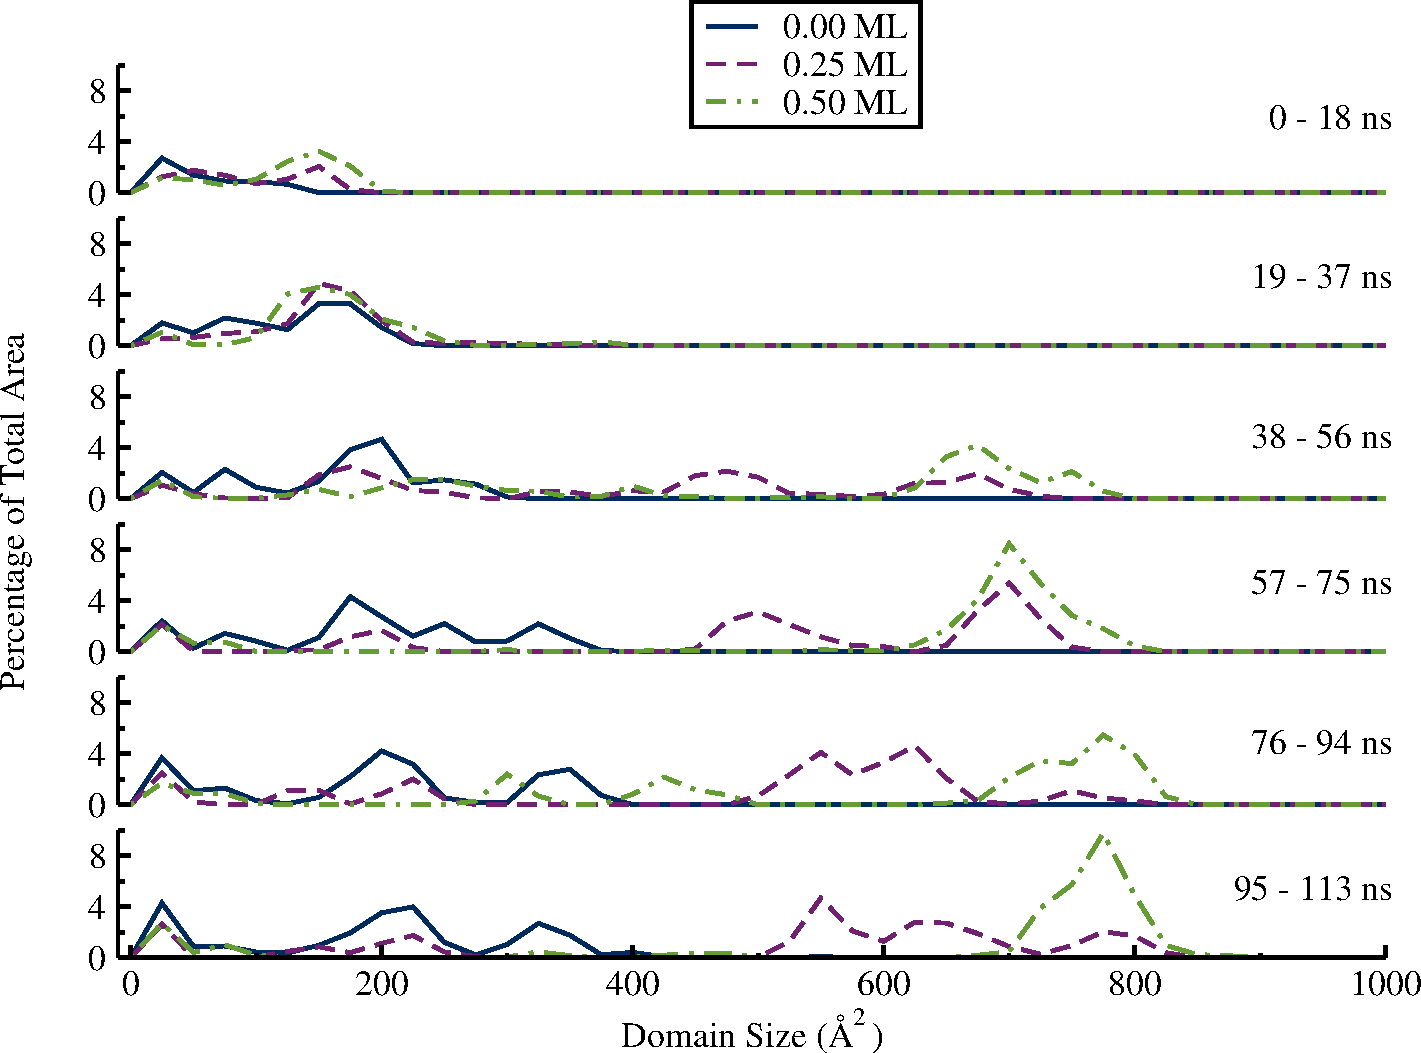
\includegraphics[width=\linewidth]{../figures/chap3/domains_Pd_110ns.pdf}
\caption{Distributions of \ce{Pd} domain sizes at different \ce{CO}
  coverages and at different times after exposure to \ce{CO}.}
\label{fig:domainAreasPd} 
\end{figure}

The appearance of \ce{Pd} from the bulk layers on the surface requires
a simultaneous reduction in the surface area of the outer \ce{Pt}
skin. Two scenarios could explain the reduction of exposed \ce{Pt}:
either the \ce{Pt} atoms are being buried under the \ce{Pd} bulk, or
islands of \ce{Pt} are forming on top of the \ce{Pd} surface.

Both mechanisms would explain the decreased \ce{Pt} surface area (see
Figure \ref{fig:domainAreasPt}).  To discern which of these mechanisms
is taking place, the identity of nearest metal atom neighbors can be
tabulated as a function of time of exposure to \ce{CO}. Single-layer
\ce{Pt} skins have atoms with 6 \ce{Pt} nearest neighbors. Islands of
\ce{Pt} require the presence of \ce{Pt} atoms with 7-9 \ce{Pt} nearest
neighbors. In Figure \ref{fig:nearestNeighbors}, we see an increase in
\ce{Pt} population with 9 \ce{Pt} nearest neighbors along with the
simultaneous decrease in \ce{Pt} atoms with only 6 \ce{Pt} nearest
neighbors.  This is evidence for the formation of multi-layer \ce{Pt}
features since single layers of \ce{Pt} are restricted to having 6
\ce{Pt} nearest neighbors.

\begin{figure}[p!]
\centering
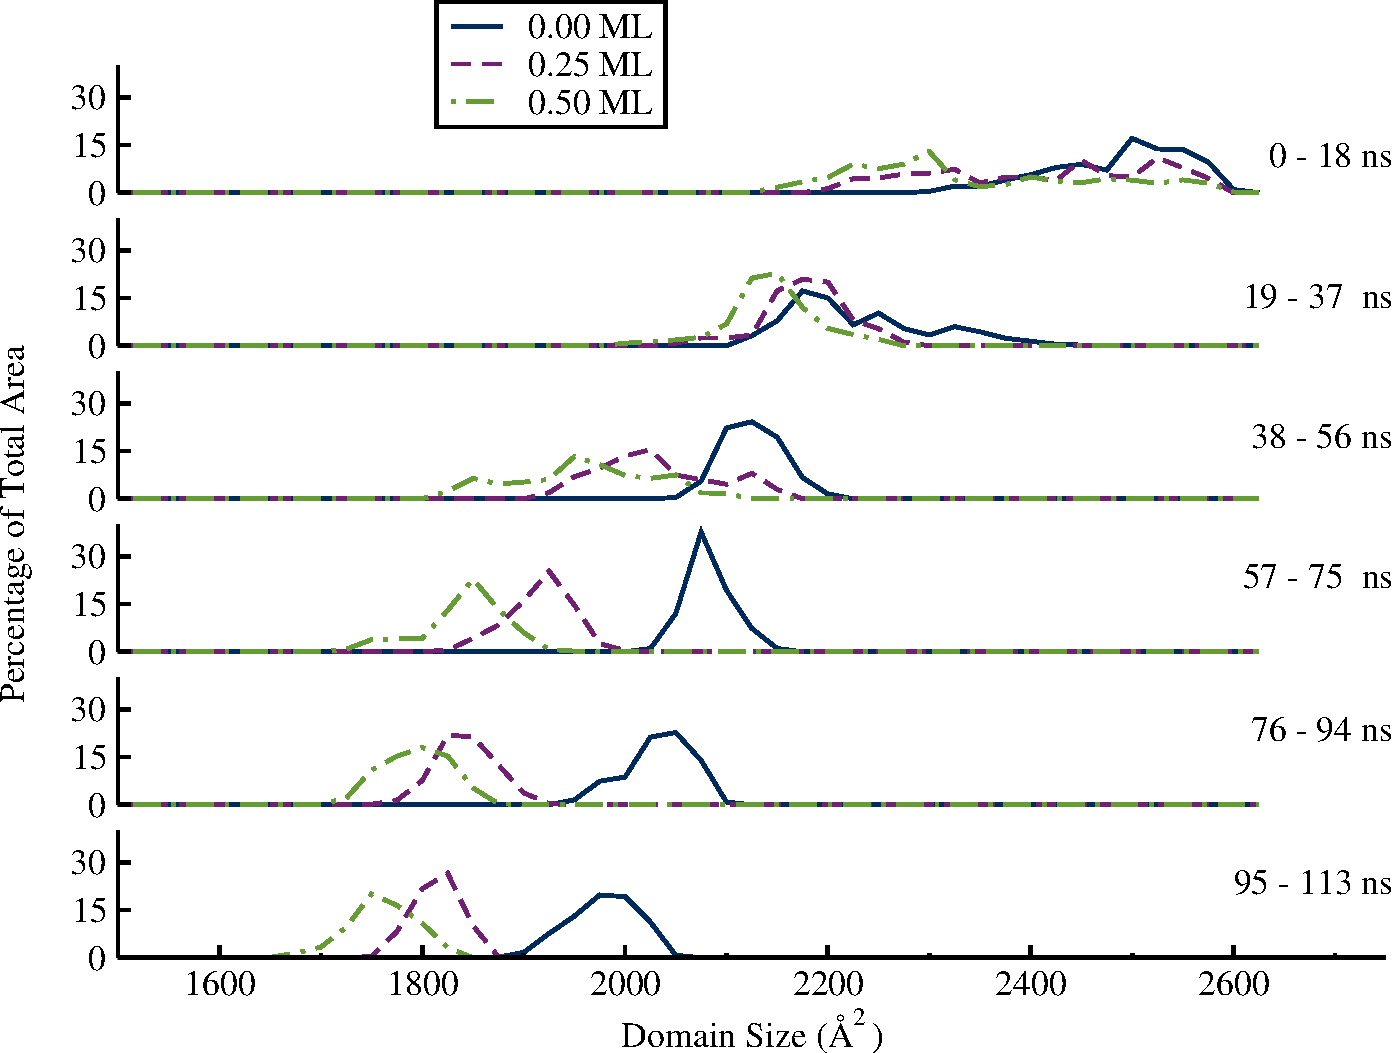
\includegraphics[width=\linewidth]{../figures/chap3/domains_Pt_110ns.pdf}
\caption{Distributions of \ce{Pt} domain sizes at different \ce{CO}
  coverages and at different times after exposure to \ce{CO}.}
\label{fig:domainAreasPt}
\end{figure}

Although it is not shown in Figure \ref{fig:domainAreasPt}, there is
an additional small peak in the \ce{Pt} graphs around 0-100~\AA,
corresponding to 1 to 2 atom clusters of \ce{Pt} embedded in the
\ce{Pd} matrix.  A figure showing the full scale of domain sizes is
supplied in appendix \ref{app:SI}.  The integrated area of
\ce{Pd}
surface coverage for each time window is shown in Table
\ref{tab:integratedArea}.

\begin{figure}[p!]
\centering
  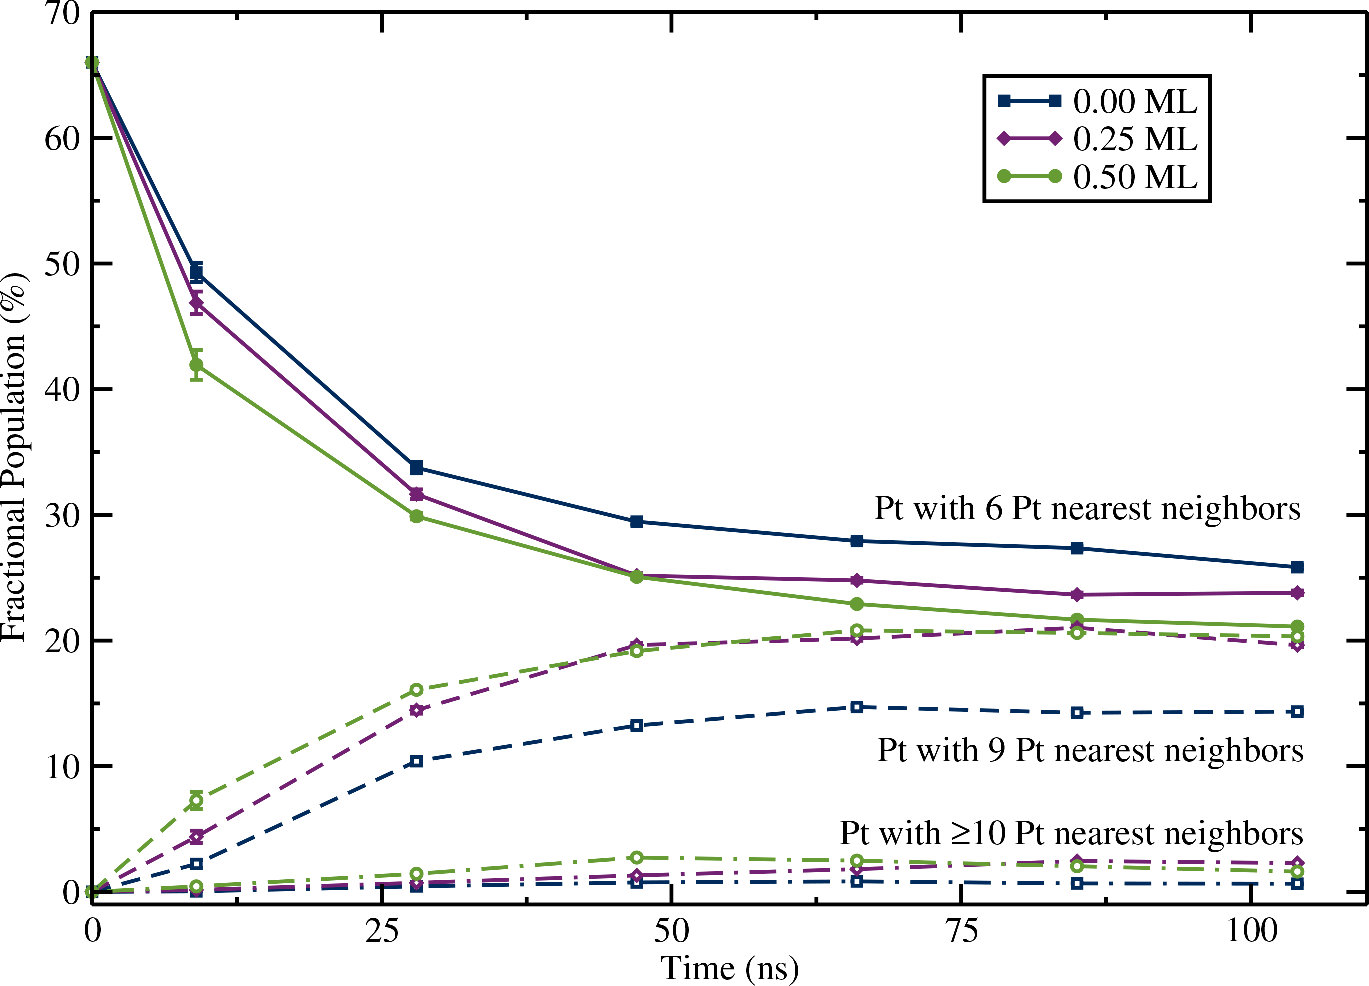
\includegraphics[width=\linewidth]{../figures/chap3/nn.pdf}
  \caption{Population of \ce{Pt} atoms with either 6 (solid), 9
    (dashed), or $\ge$ 10 (dot-dashed) \ce{Pt} nearest neighbors
    averaged over 18 ns blocks of time.  At $t=0$, the majority
    (2/3) of \ce{Pt} is located in the (111) plateaus where
    the number of \ce{Pt} nearest neighbors is 6. The remaining
    \ce{Pt} is located at step edges, with a nearest neighbor \ce{Pt}
    count of 5.} 
\label{fig:nearestNeighbors}
\end{figure}

The presence of \ce{CO} therefore appears to facilitate the clustering
of \ce{Pt} into smaller domains by forming multilayer features which
leads to a reduction of \ce{Pt} surface coverage and concomitant
increased exposure of the underlying \ce{Pd}. We note that
nearest-neighbor population analysis provides information similar to
the information one might obtain from an XAFS experiment, which could
make this phenomenon experimentally observable.

The slower restructuring observed in the bare metal system suggests
that the relative surface energies of the two metals provides the
driving force for the restructuring, while the \ce{CO} significantly
speeds up the effects (and may help to catalyze the process at lower
temperatures).

\begin{table}
%  \caption{\ce{Pd} surface coverage (as a percentage of total surface area)
%    averaged over 18 ns blocks of time.}
  \caption{CHANGE IN PD SURFACE COVERAGE AS A FUNCTION OF TIME AND CO COVERAGE}
  \begin{threeparttable}
  \begin{tabular}{c | c  c  c  c  c  c }
    \hline
    \hline
    \ce{CO} coverage  & 0-18 ns & 19-37 ns & 38-56 ns & 57-75 ns & 76-94
    ns & 95-113 ns \\
    \hline
    0.00 &  6.6 & 16.2 & 20.1 & 21.7 & 23.5 & 25.2  \\
    0.05 &  8.0 & 15.8 & 20.2 & 25.1 & 27.6 & 30.9  \\
    0.25 &  8.5 & 17.3 & 23.7 & 27.8 & 30.5 & 31.0  \\
    0.33 &  8.8 & 17.8 & 21.9 & 26.2 & 30.3 & 35.4  \\
    0.50 & 11.8 & 19.2 & 25.9 & 29.8 & 31.1 & 32.6  \\
    \hline
    \hline
  \end{tabular}
  \begin{tablenotes}
    \item The amount of Pd surface coverage is shown as a percentage of the total surface area. The individual data points are averaged over 18 nanosecond blocks of time.
  \end{tablenotes}
\end{threeparttable}
\label{tab:integratedArea}
\end{table}

Because many of the changes, both in domain size and in \ce{Pt}-atom
neighborship slow after 50~ns, this timescale appears to indicate the
onset of stable surface structures.  The presence of adsorbed \ce{CO}
hastens the onset of this quasi-equilibrium, although there is
insufficient data to predict rates from our simulations. 

\section{Discussion}
\subsection{Structural changes}
In our previous work on \ce{Pt}(557) surfaces,\citep{Michalka:2013aa} the
surface exhibited a \ce{CO}-induced structural transformation from
single steps to double steps, where the (111) plateaus effectively
doubled in size. The step coherence and orientation was preserved
following the transformation.  In the alloy case studied here, the
\ce{Pt} atoms start to cluster, breaking up the steps and causing
significant disorder on the surface.  We note, however, that the
underlying \ce{Pd} maintains the step-like structures of the (557)
interface.  A figure showing how the underlying \ce{Pd}(557) survives
the surface island formation is supplied in appendix \ref{app:SI}.


The EAM potential predicts surface energies for \ce{Pd} (111), (100),
and (110) facets that are roughly 84\% of the surface energies for the
same facets on bare \ce{Pt}.\citep{Foiles:1986ky} Although the absolute EAM
surface energies differ significantly from experimental values, the
\ce{Pd}:\ce{Pt} surface energy ratio is similar to experimental
results.\citep{Tyson:1977xe, De-Boer:1988tg} All-electron full potential
linearized augmented plane-wave (FP-LAPW) calculations have also
yielded a 0.84:1 ratio between the \ce{Pd}:\ce{Pt} (111) surface
energies.\citep{Silva:2006fk} The (557) interface has broad steps of
exposed (111), so we expect the ratio between the \ce{Pd}:\ce{Pt}
(557) surface energies to also fall close to this 0.84:1 ratio.

Because \ce{Pt} has a higher surface energy, the alloy system will
experience a driving force towards arrangements that minimize the
\ce{Pt} surface area.  Although the \ce{Pt} island formation appears
to be accelerated by the presence of adsorbed \ce{CO}, the
relationship between \ce{CO}-adsorption and the surface energies was
not initially clear. In the sections below, we discuss the effects
that the bound-\ce{CO} has on step edge stability and surface
diffusion.

We note that on \ce{Pt}(557), \ce{CO} aids in double layer formation
by lowering the barrier for an adatom on the lower plateau to burrow
into a nearby step edge.\citep{Michalka:2013aa} This burrowing lifts one
of the step edge atom onto the step above.  On the alloy surface, this
same mechanism can explain the thickening of the \ce{Pt} island layers
that is required by the 9-nearest neighbor clustering in
Figure \ref{fig:nearestNeighbors}.

\subsection{Surface adatom formation}
There is limited movement of \ce{Pd} in all of the systems we
examined. Inversions, where \ce{Pd} and \ce{Pt} atoms are swapped
between surface and subsurface layers, were observed only rarely in
the \ce{Pd}/\ce{Pt} shell, and overall the \ce{Pd} is largely
stationary.

The binding preference of \ce{CO} for bridge and hollow sites on the
\ce{Pd} surface plays a stabilizing role for step edges.  The
\ce{Pd}(557) systems show a decrease in surface roughening at higher
\ce{CO} coverages. Figure \ref{fig:PdEnergy} shows an analysis of the
energy required to move a step-edge atom into an adatom position on
the step below. In this figure, one step-edge \ce{Pd} atom is pulled
across the surface perpendicular to the step edge.  Bridging \ce{CO}
molecules adsorbed to neighbors of an edge atom will raise the barrier
that must be overcome to form a free adatom (see curves B and C in
Figure \ref{fig:PdEnergy}).

If the step-edge atom is directly bound to \ce{CO} as one part of a
bridge or hollow site, there is an even larger energetic barrier to
overcome before the adatom can be released (see curves D, E, and F in
Figure \ref{fig:PdEnergy}).

\begin{landscape}
\begin{figure}[p!]
  \centering
  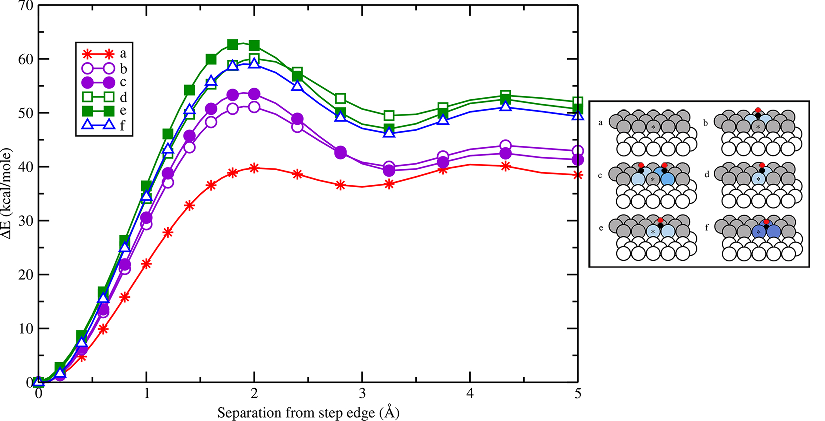
\includegraphics[width=0.85\linewidth]{../figures/chap3/PdEnergy_CO.pdf}
  \caption{The relative energies for moving a \ce{Pd} atom (marked with an
asterisk) perpendicular to a (557) step edge. This atom is translated across
the bare \ce{Pd} surface in curve A. The presence of one or two \ce{CO}
molecules bound in bridge sites near the edge stabilizes the edge atom (curves
B and C).  If \ce{CO} is bound to the edge atom in either a bridge (curves D
and E) or hollow (curve F) site, the barrier is increased.}
\label{fig:PdEnergy}
\end{figure}
\end{landscape}

This \ce{CO}-induced step stabilization is significantly different
from the \ce{Pt\bond{-}CO} interaction which favors the atop binding
position. In the \ce{Pt\bond{-}CO} case, additional bound \ce{CO} on
the surface has previously been shown to facilitate surface
roughening.\citep{Michalka:2013aa} The \ce{Pt\bond{-}CO} potential in
Table~\ref{tab:CO_parameters} has been altered from the original
parameters in Ref. \citep{Michalka:2013aa}, and Figure
\ref{fig:PtEnergy} shows that for the new potential, adsorbed \ce{CO}
can also disrupt step edges, providing an energetic benefit to
increasing the exposed \ce{Pt} surface area.

\begin{landscape}
\begin{figure}[p!]
  \centering
  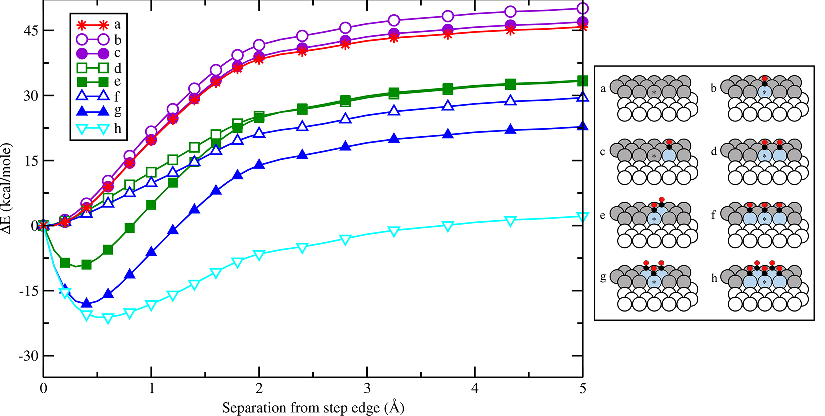
\includegraphics[width=0.85\linewidth]{../figures/chap3/PtEnergy_CO.pdf}
  \caption{The relative energies for moving a step-edge \ce{Pt} atom
    (marked with an asterisk) perpendicular to a (557) step edge.  As in
    Figure \ref{fig:PdEnergy}, the bare surface is shown in curve A.
    The presence of atop-bound \ce{CO} molecules on the edge atom and
    at nearby sites can lower the energy for adatom formation
    (e.g. curves E, G, and H).} \label{fig:PtEnergy}
\end{figure}
\end{landscape}

Based on the curves in Figs. \ref{fig:PdEnergy} and
\ref{fig:PtEnergy}, the \ce{CO} adsorbates appear to increase the
surface energy of stepped \ce{Pd} surfaces and to lower the surface
energy of equivalent \ce{Pt} surfaces.  Therefore, a kinetic mechanism
seems to be the most reasonable explanation for the enhancement of island
formation.  By effectively lowering the surface energy of the \ce{Pt},
the bound \ce{CO} increases \ce{Pt}-atom mobility.  Once the mobile
\ce{Pt} atoms find nearby islands, the surface energies still favor
compact structures, and the islands can grow more rapidly. These
islands then sit on top of a \ce{CO}-stabilized \ce{Pd} substrate.
Additionally, since the modeled \ce{Pd\bond{-}CO} binding is somewhat
stronger than \ce{Pt\bond{-}CO}, island formation exposes more of the
\ce{Pd} substrate for energetically-favorable gas adsorption.

\section{Summary}

With the simulations we have performed on \ce{Pd} and \ce{Pt/Pd} (557)
surfaces, we have been able to model the formation of \ce{Pt} islands on the
surface of a catalytically interesting alloy. It was determined that the larger
surface energies of \ce{Pt} relative to \ce{Pd} favor the segregation of
\ce{Pt} into compact domains and the beginnings of island formation were
observed even without the \ce{CO} adsorbate present on the surface. This
restructuring was primarily kinetic in nature and the presence of \ce{CO}
increased the restructuring rate by roughening the step-edges and
destabilizing the surface which lowered the potential barriers. Conversely,
the bare \ce{Pd} surface was stabilized by the \ce{CO} adsorbate because of
the preferred bridge binding and thus maintained its (557) motif throughout
the simulations.

%Our primary conclusion is that the presence of chemisorbed carbon
%monoxide can speed up the formation of \ce{Pt} islands on the surface
%of a catalytically-interesting alloy, but that this effect is largely
%kinetic in nature.  The bare \ce{Pd} surface is stabilized by the
%\ce{CO} adsorbate, while stepped \ce{Pt} surfaces are roughened and
%destabilized by the presence of the same molecule. The larger surface
%energies of \ce{Pt} relative to \ce{Pd} already favor the segregation
%of \ce{Pt} into compact domains.  At elevated temperatures, we observe
%the beginnings of island formation even without the \ce{CO} adsorbate
%on the surface, which indicates that thermodynamics favors island
%formation on this surface.
%
%The energy profiles for step-edge adatom formation in the presence of
%adsorbed \ce{CO} (see figs. \ref{fig:PdEnergy} and \ref{fig:PtEnergy})
%would seem to bring the relative surface energies closer together in
%the presence of the adsorbed \ce{CO}. Thermodynamically, this should
%destabilize \ce{Pt} islands, so our observation that the 0.5 ML
%\ce{CO} speeds up the island-formation process appears to be due
%largely to kinetics.  The lower barriers for \ce{Pt}-adatom formation
%effectively speed up the surface diffusion of \ce{Pt}.  Previous work
%on \ce{Pt}(557) surfaces showed that \ce{CO} also lowers the barrier
%for a step-burrowing mechanism that can increase the thickness of
%\ce{Pt} surface layers.\citep{Michalka:2013aa}
%
%We note that there are other catalytically-active \ce{Pt}-alloys
%(notably \ce{PtNi3} and \ce{PtNi6} nanoparticles) that display
%dealloying of \ce{Pt} upon electrochemical cycling.\citep{Tuaev:2013fk}
%In analogy to the \ce{Pd} alloy studied here, the binding of \ce{CO}
%on \ce{Ni}(111) also prefers hollow sites in preference to atop
%locations.\citep{Campuzano:1979uq} However, the surface energies of
%\ce{Ni} are close to those of \ce{Pt}, so it is not clear if our
%conclusions about the \ce{Pd}/\ce{Pt} alloy would apply to this
%system.  Further research on these alloys would require adapting the
%\ce{M\bond{-}CO} models in order to predict whether carbon monoxide
%would be a generally effective tool for concentrating
%catalytically-active \ce{Pt} sites on surface alloys.




\chapter{CARBON MONOXIDE-INDUCED RESTRUCTURING ON PLATINUM (321), (112), (765), \& (557) SURFACES}
\label{chap:facet}
%\chapter{EFFECTS OF STEP-TYPE ON THE CO-INDUCED SURFACE RECONSTRUCTIONS OF PT(557)/(112)/(321)/(765) FACETS}

%\begin{abstract}
%The effects of step-edge type and plateau length on \ce{CO}-induced
%restructuring of \ce{Pt} were explored using molecular dynamics (MD)
%simulations. Platinum systems displaying four separate facets, [(321), (765),
%(112), (557)], were constructed and exposed to various coverages of carbon
%monoxide (\ce{CO}).  Platinum-\ce{CO} interactions were parameterized from
%experimental data and Density Functional Theory (DFT) calculations, providing
%classical potentials that capture the atop binding preference on \ce{Pt}. The
%differences in binding strength between edge atoms on the various facets were
%found to play a significant role in step-edge wandering and possible
%reconstruction events. Additionally, as the mechanism for step-edge doubling
%has been seen to depend on a stochastic process of two edges meeting, the
%varying sizes of the plateaus was also found to play a large role in these
%reconstructions.  The lack of observed step-doubling on the (557) surface
%throughout the simulation time suggests that this process is quite sensitive to
%the strength of \ce{CO} binding as well as being dependent on the initial
%random meeting of two separate edges.
%\end{abstract}
%\newpage


In this chapter we explore four facets of \ce{Pt} exposed to \ce{CO} through
molecular dynamics simulations. The facets were chosen to explore the effects
plateau length and step-edge, flat or kinked, have on previously identified
reconstruction processes. The rougher, {\em i.e.} kinked, (321) and (765)
systems might be expected to undergo greater amounts of step-wandering while
also experiencing step-edge doubling at a faster rate than the previously
modeled, flat (557) systems. The change in the local coordination environment was also
examined as the surfaces underwent reconstruction, as this is an important
descriptor of potential catalytic activity. 

%\section{Introduction}
%Industrial catalysts often consist of supported metal nanoparticles or
%high-index metal surfaces as both of these materials have a high density of
%low-coordinated atoms which have been shown to be active for catalyic
%reactions.\citep{Jeong:1999aa, Larsen:1999aa} Numerous studies have examined
%catalytic activity on low-energy metal surfaces, primarily the (111), (110),
%and (100) facets which are only somewhat applicable to industrial
%conditions.\citep{Stephens:2011bv, Stamenkovic:2007kk, Mohsenzadeh:2015kx,
%?,?,?,?} However, because of the advent of High Pressure Scanning Tunneling
%Microscopy (HP-STM) and Ambient Pressure X-ray Photoelectron spectroscopy
%(AP-XPS), these systems can now be explored at higher temperatures and
%pressures which allows for a better understanding of the surface structures of
%industrial catalysts.  These roughened surfaces and nanoparticles are of
%particular interest because their predicted morphology and stability at high
%temperatures and pressures has been seen to strongly depend on the presence and
%identity of adsorbates.\citep{Tao:2008aa, Tao:2010aa, Tao:2011aa, Kim:2016cr,
%Eren:2016qt, Michalka:2013aa, Michalka:2015aa} That is, under reaction
%conditions, many of these catalysts have been observed to reconstruct, which
%can drastically change the surface of the catalyst leading to likely changes in
%the activity and selectivity of the material.
%
%One system that has received significant attention is the \ce{Pt} (557) surface
%exposed to \ce{CO}. Tao {\em et al.} using HP-STM, AP-XPS, and Density Functional
%Theory (DFT) calculations observed that by introducing carbon monoxide (\ce{CO}) to
%the system, the stepped Pt surface would undergo a step-doubling reconstruction resulting in
%step-edges that were twice as high and plateaus that were twice as long as on
%the original surface.\citep{Tao:2010aa} If the system was maintained at these conditions, the
%appearance of triangular nanoclusters bridging the steps were also eventually
%observed. After removing \ce{CO} from the system, it was found that
%these changes were reversible as the \ce{Pt} (557) surface was recovered.  It was
%suggested that this reconstruction was caused by the repulsive forces between
%adsorbed \ce{CO} molecules.  This system was also explored with molecular
%dynamics simulations and a possible mechanism to explain the step-doubling was
%proposed which also strongly depended on the \ce{CO}-\ce{CO} quadrupolar
%repulsion.\citep{Michalka:2013aa}
%
%The strong interaction of \ce{CO} with \ce{Pt} has been explored on different
%systems and similar results have been observed. Ferrer {\em et al.} examining
%\ce{Pt} (997) observed both \ce{O} and \ce{CO} induced step-doubling on the
%surface. They also saw that the presence of step-doubling was correlated with a
%factor of three increase for \ce{CO} oxidation.\citep{Balmes:2016uf} Park {\em
%et al.}, again exploring the \ce{Pt} (557) system exposed to \ce{CO}, saw that
%the ordering of the triangular nanoclusters is very sensitive to temperature
%and can undergo its own reversible restructuring separate from the doubling
%already observed on this surface.\citep{Kim:2016cr} Moving away from \ce{Pt},
%Eren {\em et al.} found that a flat (111) \ce{Cu} surface when exposed to
%\ce{CO} also underwent reconstruction, forming small nanoclusters on the
%surface that were highly active for the oxygen reduction reaction
%(ORR).\citep{Eren:2016qt} In all of these cases, the presence of adsorbates led
%to large-scale reconstructions (often reversible) of the system, however, the
%specifics of the dynamics are still being explored.
%
%Continuing in this vein, this paper examines the effect of carbon monoxide on
%various platinum facets, specifically focusing on the effect of step-type and
%plateau length. The \ce{Pt} (321) \citep{Mcclellan:1981aa, Bray:2014aa,
%Bray:2011aa}, \ce{Pt} (112) \citep{Xu:1995aa, Yates:1995aa}, \ce{Pt} (765), and
%\ce{Pt} (557) \citep{Michalka:2015aa, Michalka:2013aa, Tao:2010aa, Kim:1997aa}
%systems were chosen as they represent a mix of flat and kinked edges as well as
%short and long plateau lengths. Based on the proposed mechanism in reference
%\citenum{Michalka:2013aa}, it is hypothesized that the length of the plateau
%and the roughness of the step edge will both strongly contribute to whether
%reconstruction will occur on these surfaces.  These systems were modeled using
%classical force fields that balanced maximizing chemical accuracy, while
%simultaneously minimizing computational time.  The use of  molecular dynamics
%methods was necessary to observe the assumed long-time dynamics of these large
%systems which when previously investigated were on the order of 10s-100s of
%nanoseconds.

\section{Methodology}
Platinum-platinum interactions were modeled with the Embedded-Atom-Method (EAM)
which is described more fully in Chapters \ref{chap:PtAu} and
\ref{chap:island}.\citep{Foiles:1986ky}

%Modeling the surface reconstruction of a solid/gas interface requires large
%systems.  To observe events such as step doubling and step wandering, systems
%need to contain on the order of 10\textsuperscript{3} - 10\textsuperscript{4}
%atoms. The large number of electrons involved with this many atoms means that
%these interfaces cannot be modeled through ab {\em ab initio} molecular
%dynamics (AIMD),\citep{Kresse:1993ve, Kresse:1993qf, Kresse:1994ul}
%Car-Parrinello methods, \citep{Car:1985bh, Izvekov:2000fv, Guidelli:2000fy} or
%quantum mechanical potential energy surfaces.  In addition, the interactions
%between the individual metal atoms is poorly represented by classical pairwise
%interactions.  Therefore, the Embedded Atom Method (EAM) \citep{Foiles:1986ky}
%was used to model the \ce{Pt\bond{-}Pt} interactions.  The molecular model for
%carbon monoxide (\ce{CO}) was developed by Straub and
%Karplus,\citep{Straub:1991no} and it treats the \ce{CO} as a rigid, three-site
%body. It was chosen primarily because it describes \ce{CO}'s strong linear
%quadrupole accurately.  The \ce{Pt\bond{-}CO} interaction was modeled to match
%a combination of experimental \citep{Ertl:1977cg, Kelemen:1979ad, Yeo:1997th}
%and theoretical \citep{Feibelman:2001qa, Deshlahra:2009wu, Beurden:2002ys,
%Deshlahra:2012aa, Korzeniewski:1986kl, Mason:2004ix} data. 
%
%\subsection{Platinum-Platinum interactions}
%Since classical force fields often do not work well for transition metal
%systems, several methods have been developed that use a non-pairwise additive
%function of the local electron density.  Some of these methods include the
%embedded atom method (EAM) \citep{Foiles:1986ky, Daw:1984aq, Johnson:1989yr,
%Daw:1989ci, Plimpton:1993qi, Voter:1995ax, Lu:1997fv, Alemany:1998fp}, the
%Finnis-Sinclair method \citep{Finnis:1984hl, Sutton:1990rr} and the
%quantum-corrected Sutton Chen method \citep{Qi:1999dn}.  In general, these
%methods treat the atom as a positive core surrounded by a radially decaying
%negative charge density due to valence electrons.  The energy necessary to
%place a core at location $i$ requires knowing the electron density, $\rho_i$,
%at that point as contributed by all other metallic atoms in the system and is
%represented below, 
%
%\begin{equation}
%\rho_{i} = \sum_{j \ne i}\rho_{j}(\mathbf{r}_{ij})
%\end{equation}
%
%In the equation above, $\rho_{j}(\mathbf{r}_{ij})$ describes how the valence
%electron distribution of atom $j$ varies with the radius.  The potential from
%embedding the atom $i$ at the location in question becomes
%
%\begin{equation}
%V_{i} = F[\rho_{i}] + \sum_{j \ne i} \phi_{ij}(\mathbf{r}_{ij})
%\end{equation}
%
%In equation (2), $F[\rho_{i}]$ is a functional which describes the primarily
%attractive force between the positive core and the electron density surrounding
%the other atoms while $\phi_{ij}(\mathbf{r}_{ij})$ represents the pair-wise
%repulsion between the positively charged cores.  Potentials similar to the ones
%shown above are used in the EAM, Finnis-Sinclair, and the Quantum Sutton Chen
%methods.  These methods have been used for a variety of purposes such as
%examining bulk and nanoparticle properties, \citep{Chui:2003fk, Wang:2005qy,
%Medasani:2007uq, Mishin:1999ew} melting,\citep{Belonoshko:2000jk,
%Sankaranarayanan:2006ye, Sankaranarayanan:2005bh} fracture,
%\citep{Shastry:1996qg, Shastry:1998dx, Mishin:2001qt} crack propagation,
%\citep{Becquart:1993sr} and alloying dynamics.  \citep{Shibata:2002hh,
%Mishin:2002if, Zope:2003ai, Mishin:2005vc} EAM's parameterization included
%second and third nearest-neighbor interactions which makes it particularly
%suited to systems that are expected to deviate from low-energy (111) surfaces,
%which is why it was chosen to describe the \ce{Pt\bond{-}Pt} interactions of
%our high-index surfaces.  \citep{Foiles:1986ky} 

\subsection{Carbon Monoxide model}
The carbon monoxide model developed by Karplus and Straub\citep{Straub:1991no},
which was discussed in Chapter \ref{chap:PtAu} and shown in Table \ref{tab:CO}
is used here without change.
%The large linear quadrupole moment of \ce{CO} is believed to play a primary
%role in the reconstruction of \ce{Pt} (557)\citep{Tao:2010aa, Michalka:2013aa}
%and since Karplus and Straub's model captures that quadrupole it was chosen for
%this work.\citep{Straub:1991no} This model consists of three rigid sites, 2
%atomic describing the \ce{C} and \ce{O} both with an attached negative charge
%and a massless site at the center of mass that carries a large positive charge.
%The necessary parameters are shown in Table \ref{tab:parameters}.  These
%parameters still produce a small dipole moment of 0.35 D while keeping the
%linear quadrupole (-2.40 D\AA) close to both experiment (-2.63 D\AA)
%\citep{Chetty:2011dp} and quantum mechanical predictions (-2.46 D\AA).
%\citep{Rizzo:2000sp}

%\begin{table}
%\caption{PARAMETERS FOR THE CO MODEL}
%%\caption{Positions, Lennard-Jones parameters ($\sigma$ and $\epsilon$) and charges for \ce{CO\bond{-}CO} interactions}
%\centering
%\begin{threeparttable}
%\centering
%\begin{tabular}{c c c c c}
%\hline
%\hline
% & z \tnote{a} & $\sigma$ \tnote{a} & $\epsilon$ \tnote{b} & q \tnote{c}\\
% \hline
% C & -0.6457 & 3.83 & 0.0262 & -0.75 \\
% O & 0.4843 & 3.12 & 0.1591 & -0.85 \\
% M & 0.0 & & & 1.6 \\
%\hline
%\hline
% \end{tabular}
%\begin{tablenotes}
%  \item \ce{CO\bond{-}CO} cross-interactions are modeled with Lennard-Jones potentials.
%  \item[a] Positions are given in \AA
%  \item[b] Energies are given in kcal/mol
%  \item[c] Charges are given in elementary units, $e^{-}$
%\end{tablenotes}
%\end{threeparttable}
%\label{tab:parameters}
%\end{table}

\subsection{Platinum-Carbon Monoxide interactions} The extensive experimental
\citep{Ertl:1977cg, Kelemen:1979ad, Ertl:1989, Schweizer:1989fk, Szanyi:1992aa,
Yeo:1997th} and theoretical \citep{Feibelman:2001qa, Deshlahra:2009wu,
Beurden:2002ys, Deshlahra:2012aa, Korzeniewski:1986kl, Mason:2004ix} work on
\ce{Pt\bond{-}CO} allows for significant data upon which to parameterize this
interaction.  The \ce{Pt\bond{-}CO} interaction has been
modified from previous models\citep{Michalka:2013aa, Michalka:2015aa} to better
capture the difference in energy between the preferred atop and bridge sites as
described by DFT calculations.\citep{Deshlahra:2012aa} The model has also been
modified to use a purely repulsive Morse potential to represent the
\ce{Pt\bond{-}O} interaction in contrast with previous
implementations.\citep{Korzeniewski:1986kl, Michalka:2013aa} Using a purely
repulsive Morse prevents unphysical \ce{O} binding to the surface.
Combining the Lennard-Jones \ce{Pt\bond{-}C} interaction with the repulsive
Morse describing the \ce{Pt\bond{-}O} interaction, provides the following
potential form for the \ce{Pt\bond{-}CO} interaction,

\begin{equation}
V_{r} = 4\epsilon\bigg(\Big(\frac{\sigma}{r_{Pt-C}}\Big)^{12} - \Big(\frac{\sigma}{r_{Pt-C}}\Big)^{6}\bigg) + D_{e}e^{-2\gamma(r_{Pt-O}-r_{e})}
\end{equation}

Table \ref{table:pt-co} shows the parameters for the above potential, while
Table \ref{table:sites} provides the binding energies for the various sites
based on these parameters and compares them to DFT\citep{Deshlahra:2012aa} and
experimental data.\citep{Ertl:1977cg, Kelemen:1979ad}

\begin{table}
\caption{REFIT PARAMETERS FOR THE PT-CO CROSS-INTERACTIONS}
%\caption{Parameters for Pt-CO Interaction}
\centering
\begin{threeparttable}
\centering
\begin{tabular}{c c c c c}
\hline
\hline
\multicolumn{2}{c}{Pt-C} & \multicolumn{3}{c}{Pt-O}  \\
\hline
$\sigma$\tnote{a} & $\epsilon$\tnote{b} & $r_{e}$\tnote{a} & $\mathrm{D}_e$\tnote{b} & $\gamma$\tnote{c} \\
\hline
1.68 & 52.25 & 5.15 & 0.03 & 1.7 \\
\hline
\hline
\end{tabular}
\begin{tablenotes}
  \item Metal-C interactions are modeled with Lennard-Jones potentials, while the metal-O interactions were fit to Morse potentials.
  \item[a] Distances are given in \AA
  \item[b] Energies are given in kcal/mol
  \item[c] $\gamma$ is given in units of \AA\textsuperscript{-1}
\end{tablenotes}
\end{threeparttable}
\label{table:pt-co}
\end{table}

\begin{table}
\caption{ADSORPTION ENERGIES FOR CO ON PT(111) WITH NEW PARAMETERIZATION}
%\caption{Pt-CO Binding Site Preferences (eV)}
\centering
\begin{threeparttable}
\centering
\begin{tabular}{c c c c}
\hline
\hline
& Atop & Bridge & Hollow \\
\hline
This work & -1.49 & -1.36 & -1.32 \\
DFT\tnote{a} & -1.48 & -1.47 & -1.45 \\
Experimental\tnote{b} & -1.43 & & \\
\hline
\hline
\end{tabular}
\begin{tablenotes}
  \item All binding energies are given in eV.
  \item[a] Ref. \citep{Deshlahra:2012aa}
  \item[b] Refs. \citep{Ertl:1977cg, Kelemen:1979ad}
\end{tablenotes}
\end{threeparttable}
\label{table:sites}
\end{table}


\subsection{Systems}

The stepped \ce{Pt} systems were created so as to be of a similar size, and fit
properly in an orthorhombic periodic box. The four surface cuts were doubled
in either the $x$ or the $y$ direction so that the effect of step lengths could
also be investigated and were identified as LS, for systems with longer steps,
and MS, for systems with more steps. The system dimensions, number of atoms,
and surface coverages are enumerated in Table \ref{tab:dimensions}. Each system
began as a FCC crystal and was cut to expose the desired face in the extended
$z$ axis, while staying periodic along the $x$ and $y$ axis.
%the pt(112) systems were
%8 layers thick, had a slab thickness of $\sim$18 \aa~and were in boxes of 65.70
%x 54.24 x 100 \aa~and 32.82 x 108.4 x 100 \aa.  the pt(557)
%systems were 10 layers thick, had a slab thickness of $\sim$21 \aa~ and were in
%boxes of 55.27 x 49.48 x 100.3 \aa~and a 110.6 x 24.76 x 100.3
%\aa.  the pt(321) systems were 8 layers thick, had a slab thickness of
%$\sim$18 \aa~and were in boxes of 35.82 x 95.49 x 100 \aa~and 71.70 x
%47.71 x 100 \aa. the pt(765) systems were 9 layers thick, had a slab
%thickness of $\sim$19 \aa~and were in boxes of 58.36 x 50.19 x 100 \aa~
%and 28.72 x 100.5 x 100 \aa.  

\begin{table}
\caption{SYSTEM DIMENSIONS FOR THE STEPPED PT SURFACES}
%\caption{Dimensions}
\centering
\begin{threeparttable}
\centering
\begin{tabular}{c c c c c}
\hline\hline
Surface & Atoms & Surface Atoms & \multicolumn{2}{c}{System dimensions\tnote{a} (MS \& LS)}  \\ 
\hline
(321) & 4440 & 720 & 71.7 x 47.7 x 100 & 35.8 x 95.5 x 100  \\
(112) & 4608 & 768 & 32.9 x 108.5 x 100 & 65.8 x 54.3 x 100 \\
(765) & 3744 & 792 & 28.7 x 100.5 x 100 & 58.4 x 50.2 x 100 \\
(557) & 3888 & 720 & 110.6 x 24.8 x 100 & 55.3 x 49.5 x 100 \\
\hline
\hline
\end{tabular}
\begin{tablenotes}
  \item Systems were replicated in either the $x$ or $y$ dimension at the
beginning of the simulations to examine the effect of edge length and quantity
of steps on the reconstruction process.
  \item[a] Box dimensions are given in \AA
\end{tablenotes}
\end{threeparttable}
\label{tab:dimensions}
\end{table}

The systems were then run in the canonical (NVT) ensemble, gradually raising
the temperature to either 700\ ~K or 1000\ ~K depending on the initial
stability of the pure system.  The systems with longer plateaus were more
stable and were run at 1000\ ~K to bring reconstruction dynamics into the
domain of typical simulation times.  Gas phase CO molecules, corresponding to
0.25 ML or 0.5 ML surface coverage were placed in the vacuum region and then
allowed to adsorb on the surface. The systems were then re-equilibrated for
approximately one nanosecond before data collection was begun.  Data was
collected by running the systems in the microcanonical (NVE) ensemble for 100
ns.  Simulations were performed using the open source molecular dynamics
package, OpenMD.\citep{Fennell:2006xq, Meineke:2005pt, openmd} 

\section{Results}

%\subsection{Diffusion}
%Make a table... hopefully the burrowing will explain most of this
%Additionally, when double steps (or partial double steps form) there is not as much movement afterwards, so that is a possible explanation as well
% Try to show a count of mobile atoms (as a function of time maybe)

\subsection{Generalized coordinate number}
Many catalytic reactions have a degree of structural sensitivity such that only
a subset of the displayed atoms on a roughened surface or nanoparticle are
actually catalytically active. While the coordination number of individual
atoms can help describe their binding strengths, Calle-Vallejo {\it et al.}
have observed that including the first and second nearest neighbor counts in
their description of coordination allowed for a better description of an atom's
local environment.\citep{Calle-Vallejo:2015qq} With this information, similar to
volcano plots, they were able to create ``coordination-activity plots'' that
related an atoms coordination with its catalytic activity. Since they needed to
include information about second nearest neighbors, they introduced a new term,
the generalized coordination number (GCN) as a useful measure of the various
binding environments on metal surfaces or nanoparticles. 

\begin{equation}
  \overline{CN}(i) = \sum_{j=1}^{n_i}\frac{cn(j)}{cn_{\textrm{max}}}
  \label{eq:gcn}
\end{equation}

The GCN is a straight-forward extension of a nearest-neighbor analysis with the
primary difference being that the GCN of an atom $i$, $\overline{CN}(i)$,  is
calculated from the average of the coordination numbers, $cn(j)/cn_\term{max}$,
of its nearest neighbors.  The sum is over atom $i$'s first nearest neighbors
and $cn_\textrm{max}$ is a normalization term and for an FCC crystal is equal
to 12, the bulk coordination number.

\begin{figure}[p!]
  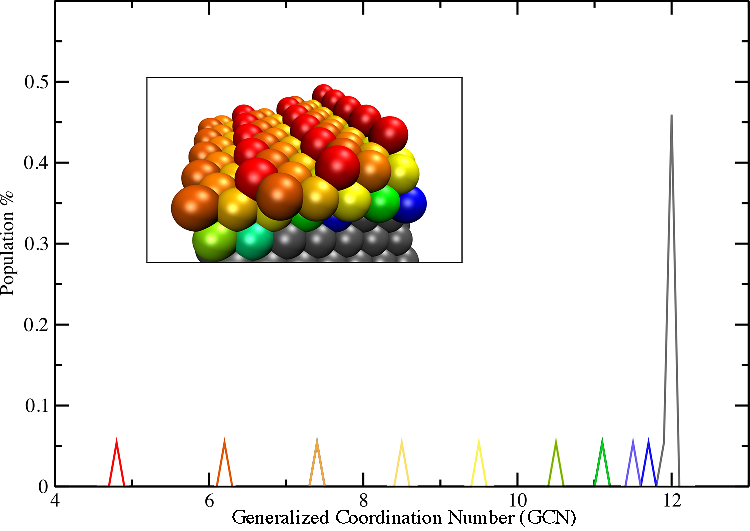
\includegraphics[width=\linewidth]{../figures/chap4/321_ideal_gcn.pdf}
  \caption{A graph of the generalized coordinate numbers of an ideal Pt(321)
system colored to match the inset figure. Other than the bulk (GCN=12), the
ideal (321) surface displays a wide variety of environments for its surface
atoms.  The edge atoms (red) have the lowest GCN because they are 
under-coordinated, whereas the plateau atoms have GCN's around the ideal
surface number of 7.5. Subsurface atoms (yellow, greens, and blues) have a
larger GCN then the surface, but are still less than the bulk GCN of 12.  }
\label{fig:ideal321GCN}
\end{figure}

The concept is further illustrated in Figure \ref{fig:ideal321GCN} where we see
an ideal \ce{Pt} (321) surface color coded to match the encompassing GCN graph.
The bulk atoms (GCN=12) make up the majority of the system, however, there is a
wide range of potentially catalytically active sites on the surface.
Specifically, Calle-Vallejo {\em et al.} argued that for the Oxygen Reduction
Reaction (ORR) a \ce{Pt} atom with a GCN of $\sim$8.3 would be the most
catalytically active site. Since an ideal (111) surface in composed of atoms
with a GCN of $7.5=(6\times9 + 3\times12)/12$, this implies that surfaces that
display some amount of concavity may be necessary to achieve the highest
catalytic activities. Another color-coded graph of an ideal \ce{Pt} (557)
system is included in Appendix \ref{app:SI2} as Figure \ref{fig:557GCN} to
highlight the differences between a rough surface, (321), to a comparatively
flat surface, (557).

In Figure \ref{fig:LS321GCNF}, we see GCN data from the \ce{Pt} (321) systems
which are focused on the surface and subsurface layers, i.e. non-bulk, for the
three examined coverages at  the beginning and end of the simulation times. The
growth in the peaks around 7.5, as highlighted with the blue bar, suggest that
the surface is reconstructing, displaying larger (111) domains. The amount of
CO present in the system plays a direct role in this reconstruction.
Additionally, the decrease in peaks at 4.5 and 6.2 provide evidence of the
system moving to a lower energy facet.  The growth in the peak at a GCN of 11.2
shows how the subsurface layers are becoming more bulk-like.

\begin{figure}[p!]
  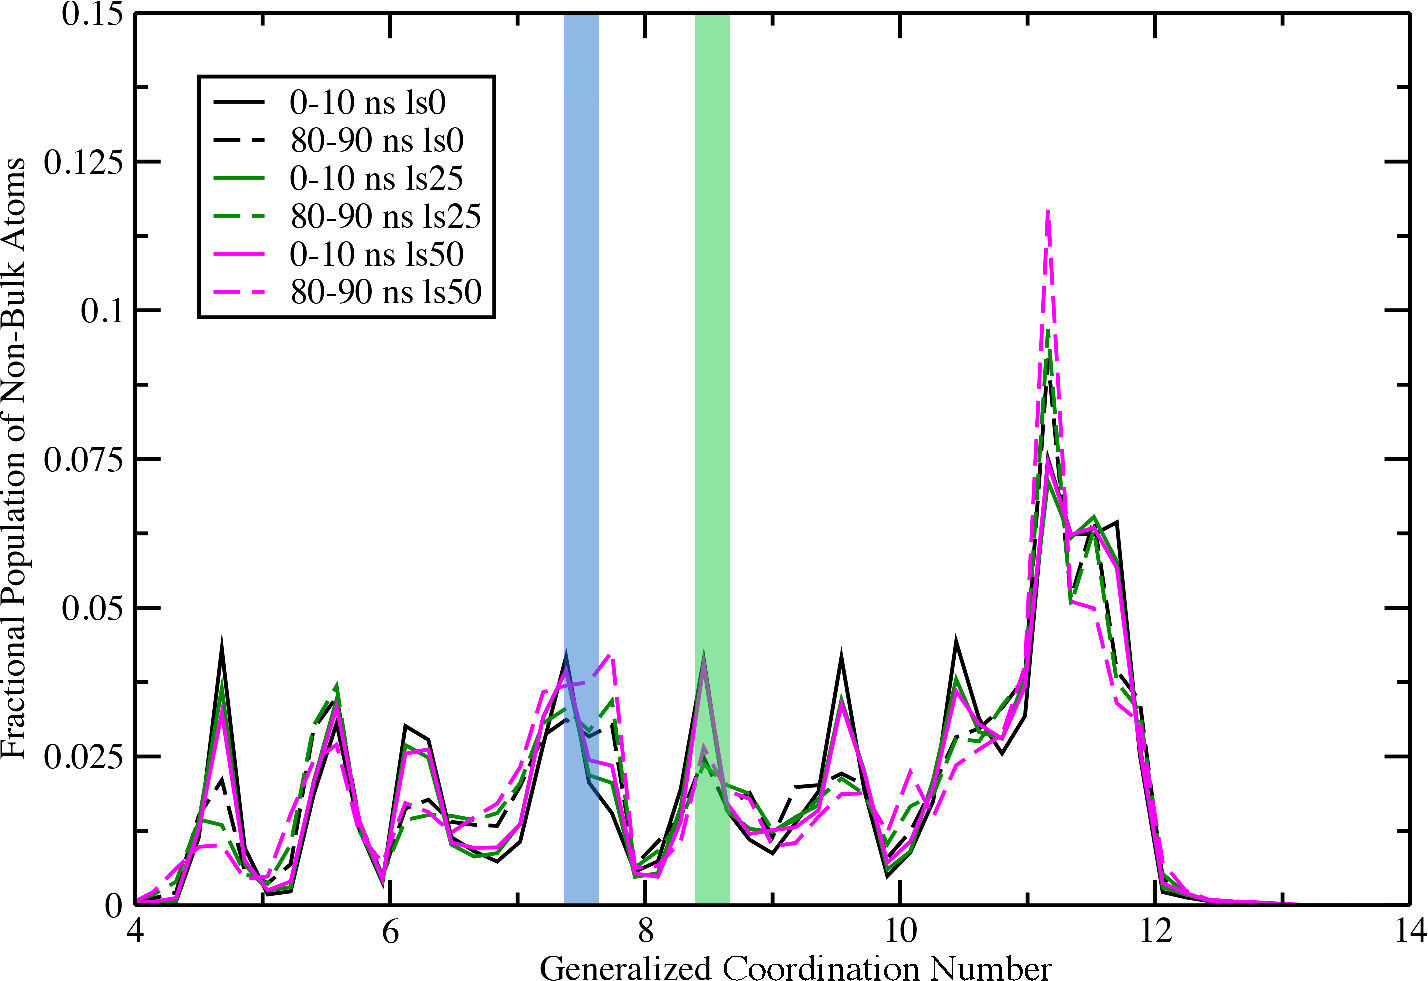
\includegraphics[width=\linewidth]{../figures/chap4/321ls_GCNF.pdf}
  \caption{Plots of the average GCN for the non-bulk atoms of the \ce{Pt} (321)
LS systems.  Solid lines represent the averaged GCN during the first 10
nanoseconds of simulation time, while the dotted lines corresponds to a time near
the end of the simulations. Black lines indicate the bare 0 ML system, while
green and magenta depict the 0.25 ML and 0.5 ML systems respectively. The blue
bar is aligned at a GCN=7.5 which corresponds to the GCN of a surface atom in
an ideal \ce{Pt} (111) surface, while the green bar highlights the region
identified by Calle-Vallejo {\em et al.} as being especially active for ORR
activity.\citep{Calle-Vallejo:2015qq}}
\label{fig:LS321GCNF}
\end{figure}

The other systems examined in this study experienced much less reconstruction,
as evidenced in their GCN plots. Figure \ref{fig:LS112GCNF} shows the
calculated GCN's of the \ce{Pt} (112) LS systems and the minimal changes that
the system exhibited during the simulation. There is a slight reduction of
population around 5.5 which is consistent with the step sinking that was
observed on some of these systems. Representative GCN plots of the other
systems are included in Appendix \ref{app:SI2} as Figures \ref{fig:557lsGCN}
through \ref{fig:765lsGCN}.

\begin{figure}[p!]
  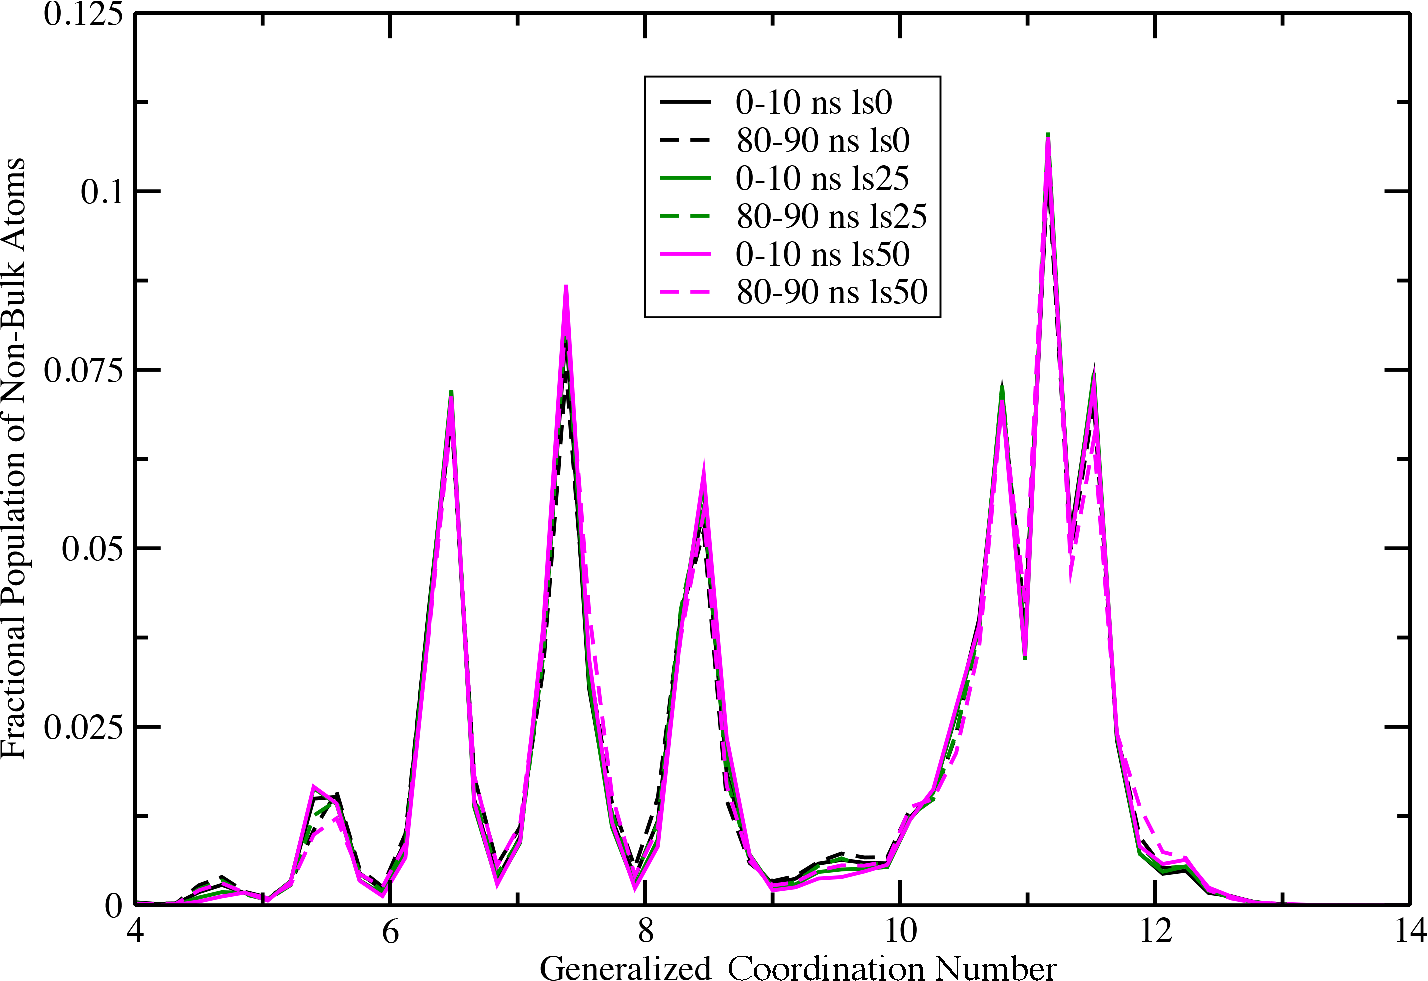
\includegraphics[width=\linewidth]{../figures/chap4/112ls_GCNF.pdf}
  \caption{Plots of the average GCN for the non-bulk atoms of the Pt (112) LS
systems. Solid lines represent the averaged GCN during the first 10 nanoseconds
of simulation time, while the dotted lines correspond to a time near the end of
the simulations. Black, green and magenta lines depict the 0, 0.25, and 0.5 ML
systems respectively. Except for a slight shrinking of the peak at 5.5 combined
with some growth at 9.5 and around 12, the local environment of this system is
barely perturbed.}
\label{fig:LS112GCNF}
\end{figure}

\subsection{Edge wandering}
All of the surfaces experienced some amount of step-wandering which will be
discussed by facet below.

\subsubsection{Pt (557)}
The (557) surfaces have been explored more fully in previous
papers,\citep{Tao:2010aa, Michalka:2013aa}, but we must  report that no
doubling was observed during the simulation time despite the large degree of
step wandering. The two most likely explanations include the stochastic nature
of this reconstruction. Additionally, the \ce{Pt\bond{-}CO} interaction has
been weakened compared to the fit in the previous paper.\citep{Michalka:2013aa}
It is likely that both of these explanations are contributing factors as there
was significant step-wandering, but the key event (two step-edges meeting) did
not occur for any of the (557) systems simulated in this study.

\subsubsection{Pt (112)}
The (112) MS surfaces exhibited restructuring to relieve residual surface tension.
This resulted in a number of the
originally (100) step edges sinking into the surface and shifting
sideways to display a sunken (111) step edge. This is highlighted in Figure
\ref{fig:112sunken} in Appendix \ref{app:SI2}.  Adatom formation from these (111)
steps was minimal and the total amount of adatom creation and movement on
these systems was much less than on the (112) systems with longer steps. 

The (112) LS surfaces exhibited moderate step-wandering, although limited
step-edge reconstructions were observed. Some of the steps on each system sunk
into the bulk, making adatom formation difficult.  The bare surface maintained
its displayed (112) step-edges macroscopically.  We also observed that there
was significant adatom ejection and re-adsorption on the surface. The presence
of \ce{CO} increased the disruption of the step-edges and the largest amount of
restructuring in these systems was observed on the 0.5 ML system.  Three steps
in this system coalesced into a mini-(111) facet, highlighted in Figure
\ref{fig:tripleStep}.

\begin{figure}
\centering
  \includegraphics[width=0.8\linewidth]{../figures/chap4/112_tripleStep.pdf}
  \caption{Top-down view of the (112) 0.5 ML surface extended to display longer
steps. (a) depicts the system at the beginning of the run when minimal
step-wandering had occurred. (b) Near the end of the simulation, three edges
had begun to coalesce into a triple step, highlighted in yellow.}
  \label{fig:tripleStep}
\end{figure}

\subsubsection{Pt (765)}
The (765) surfaces, while undergoing significant amounts of step-wandering did
not experience any clear instances of step-edge doubling during the
simulations. The MS systems, those extended to display wider steps maintained
the (765) motif over the entire simulation (barring one incident on the 0.5 ML
system). What appears to be the initial stages of a doubling event results in
portions of both involved edges sinking into the surface of the metal. This
process is shown in Figure \ref{fig:765Edge} in Appendix \ref{app:SI2}.

The LS systems also experienced significant step-wandering. While no doubling
was observed, connections between separate edges were seen. However, these
connections led to some of the steps rotating on the surface of the metal.
Despite the apparent stability of the (765) motif for the MS systems, the 0 and
0.5 ML LS systems appeared to undergo an unstructured reconstruction that lead
to an increase of the GCN at 6.8 highlighted in Figure \ref{fig:765lsGCN}.

\subsubsection{Pt (321)}
The (321) steps showed the most interesting behavior. Numerous instances of
step doubling were observed on both the MS and LS 0.5 ML systems. The 0.25 ML
systems also showed minor reconstruction, although little doubling
was observed. The 0 ML systems did experience a small amount of step-wandering,
likely due to the high energy of the surface and the elevated temperatures the
systems were run at.

An interesting case of frustrated double layer formation is highlighted in
Figure \ref{fig:partialDoubleLayer} where three double layers have begun to
form, but the center double layer highlighted in green is preventing the blue
or yellow double layer from coalescing. Within our simulation time, the 0.5 ML
LS systems were not observed to form a double step that encompassed the length
of the system, whereas numerous examples of partial double steps can be found.

\begin{figure}
\centering
\includegraphics[width=0.6\linewidth]{../figures/chap4/321_partialDoubleLayer.pdf}
\caption{Images of the (321) 0.5 ML long-step systems at the (a) beginning and
(b) end of the simulation time. Before \ce{CO} is added to the system the
kinked edges are well maintained barring slight dislocations. After a
significant amount of simulation time, \ce{CO} induces double step formation.
The plateaus are narrow enough that the initial step of this process, forming a
``nucleation'' site can happen numerous times between separate steps.
Highlighted in (b) are frustrated double layers, where any ``zippering'' that
would be expected to finish the formation of a double layer is hindered by the
resultant un-zippering of another layer.}
\label{fig:partialDoubleLayer}
\end{figure}

While there was a significant amount of step-wandering observed on the (321)
0.25 LS surface, the system appeared to get trapped in a meta-stable state
highlighted in Figure \ref{fig:diamonds}. There is a small amount of step-edge
doubling in these systems, but the majority of the system is taken up by small
diamond shaped (111) domains. The formation of so many nucleation sites between
step edges may suggest a possible reason for the pausing at this configuration
and will be explored in more detail in the discussion.

\begin{figure}
\centering
\includegraphics[width=0.6\linewidth]{../figures/chap4/321MiniDiamonds.pdf}
\caption{The (321) LS 0.25 ML system at (a) the beginning of the simulation and
(b) at the end. The green diamonds highlight the repeated (111) domains formed
between the initially regular steps. The presence of so many nucleation sites,
where two edges touch at one to two atoms may purely be a result of energetics
of the (321) step surface.}
\label{fig:diamonds}
\end{figure}

\section{Discussion}
Based on the results of our previous work\citep{Michalka:2013aa}, we predicted
that all of these systems would have a high likelihood of undergoing
double-layer reconstruction. While the amount of step-wandering was significant
for the majority of the systems exposed to \ce{CO}, only the (321) surfaces
demonstrated repeated step-edge doubling. One explanation for this surprising
result is that our modification of the \ce{Pt\bond{-}CO} forcefield to bring it
closer to experimental results weakened the \ce{Pt\bond{-}CO} step energetics
in these systems. Here we will discuss the features of the forcefield and the
studied systems while also examining the effects of step type and plateau
length on step-wandering.

\subsection{Surface energy}
Surface energies were calculated for every system that was studied, as well as
for the low-index Pt(111), Pt(100), and Pt(110) surfaces.  To perform these
calculations, systems were created such that they were periodic in all
directions ({\em x, y, z}). The desired surface was then exposed by extending
the box size in the {\em z}-direction sufficiently to prevent long-distance
interactions between steps.  The change in the potential energy that resulted
was used to calculate the surface energy.  The values calculated for the
low-energy surfaces matched previous values calculated using EAM, which is
expected as they were one of many experimental variables that were used to
parameterize the EAM forcefields.\citep{Foiles:1986ky} These values differ
slightly from experimental\citep{Tyson:1977xe, De-Boer:1988tg, Galeev:1980pt} and
DFT\citep{Vitos:1998qq} sources, but match in terms of proportions between the
various surfaces.  The surface energies of Pt(111), Pt(110), and Pt(100) that
were calculated in this experiment are compared to those calculated in previous
EAM experimentation \citep{Foiles:1986ky} as well as against experimental
surface energy values in Table \ref{table:lit_surface_energy}.

\begin{table}
\caption{SURFACE ENERGY VERIFICATION OF LOW-INDEX PT SURFACES}
%\caption{Surface Energy Verification}
\centering
\begin{threeparttable}
\centering
\begin{tabular}{c c c c c }
\hline
\hline
Facet & Surface Energy & EAM\tnote{a} & Experimental\tnote{b} & Simulated/Experimental\\
\hline
\ce{Pt} (111) & 1.43 & 1.44 & 0.977 & 1.46 \\
\ce{Pt} (100) & 1.63 & 1.65 & 1.286 & 1.27 \\
\ce{Pt} (110) & 1.75 & 1.75 & 1.553 & 1.13 \\
\hline
\hline
\end{tabular}
\begin{tablenotes}
  \item All energies are given in J/$\textrm{m}^2$
  \item[a] Ref. \citep{Foiles:1986ky}
  \item[b] Ref. \citep{Galeev:1980pt}
\end{tablenotes}
\end{threeparttable}
\label{table:lit_surface_energy}
\end{table}

The same methodology was used to calculate surface energies for the \ce{Pt}
(765), \ce{Pt} (557), \ce{Pt} (112), and \ce{Pt} (321) surfaces and are shown
in Table \ref{table:surface_energy}.  The surface energy of these systems is
inversely correlated to the distance between step-edges. This is reasonable as
the larger step length corresponds to a larger amount of the low-energy (111)
facet being displayed. This suggests that the higher surface energy systems
will be more amendable to reconstruction as they can then display a greater
proportion of (111) domains.

\begin{table}
\caption{SURFACE ENERGY AND STEP-LENGTH CALCULATIONS FOR MODELED PT SURFACES}
%\caption{Surface Energy}
\centering
\begin{threeparttable}
\centering
\begin{tabular}{c c c}
\hline
\hline
Facet & Surface Energy\tnote{a} & Step Separation\tnote{b} \\
\hline
%pt(765) & 1.525686968 & 16.79333333 \\
%pt(557) & 1.546605208 & 13.785 \\
%pt(112) & 1.673338459 & 6.79 \\
%pt(321) & 1.756522657 & 5.901440476 \\
\ce{Pt} (765) & 1.53 & 16.79 \\
\ce{Pt} (557) & 1.55 & 13.79 \\
\ce{Pt} (112) & 1.67 & 6.79 \\
\ce{Pt} (321) & 1.76 & 5.90 \\
\hline
\hline
\end{tabular}
\begin{tablenotes}
  \item[a] Energies are given in J/$\textrm{m}^2$
  \item[b] Distances are given in \AA
\end{tablenotes}
\end{threeparttable}
\label{table:surface_energy}
\end{table}

\subsubsection{Plateau length}
In addition to the plateau length providing a good measure of the surface
energy of these facets, the length of the plateau also plays a role in the
mechanism of restructuring. The mechanism for doubling as proposed in reference
\citep{Michalka:2013aa} and mentioned previously, is strongly dependent on
two step-edges meeting and forming a stable nucleation site from which a
``zippering'' process can speed up the rest of the reconstruction. As the
meeting of two step-edges is primarily a stochastic process, anything that
makes the initial meeting less likely, like increasing the distance between
steps, will make the reconstruction process more difficult to capture with our
finite simulation times. This combined with the retuning of the
\ce{Pt\bond{-}CO} forcefield, explains why despite seeing significant
step-wandering on the (557) and (765) systems little to no reconstruction was
observed during the 100 ns of simulation, whereas the (321) surfaces exhibited 
many doubling events. This would suggest that the (112) surface should also
have seen significant doubling, and while there was one instance of a triple
step beginning to form, the slight reconstruction that sunk a number of the
step-edges made any sort of adatom formation on those surfaces difficult.
Recreating the (112) systems and relieving residual surface tension 
would likely lead to a larger amount of step doubling.

\subsection{Energy to separate from edge}
As the formation of adatoms is essential for step-wandering and step-doubling,
energy curves describing this process were computed for several \ce{CO}
configurations, as had been done previously.  \citep{Michalka:2013aa,
Michalka:2015aa} These calculations were performed at various displacements as
the atoms of interest were moved perpendicular to the step edge along the
plateau as shown in Figures \ref{fig:112_557_ES} and \ref{fig:321_765_ES}. The
strong quadrupolar repulsion between aligned \ce{CO} leads to this process of
adatom formation becoming energetically favorable at high coverages. For the
faceted (112) and (557) systems, configurations e, g, and h, highlighted in
Figure \ref{fig:112_557_ES}, make the initial formation of an adatom an
energetically favorable process. The (321) and (765) facets examined in Figure
\ref{fig:321_765_ES}, owing primarily to their rougher step edges, show that
configurations e, f, g, and h are all favorable for adatom formation.

\begin{landscape}
\begin{figure}[p!]
  \centering
  \includegraphics[width=0.75\linewidth]{../figures/chap4/112_557_EnergySeparation.pdf}
  \caption{Energies for displacing an edge atom (*) perpendicularly from the
step edge. The top graph contains data for the (112) surface while the bottom
graph depicts results for the (557) surface.  Each of the energy curves
corresponds to one of the labeled configuration to the right and are referenced
to the unperturbed step edge. The white spheres represent Pt atoms on the upper
step, while the dark grey spheres are Pt on the lower step.  The colored atoms
(blue) on the upper step represent a Pt atom with a CO molecule adsorbed at an
atop site. Certain configurations of CO, notably g and h, can lower the
energetic barrier for creating an adatom.}
\label{fig:112_557_ES}
\end{figure}
\end{landscape}

\begin{landscape}
\begin{figure}[p!]
  \centering
  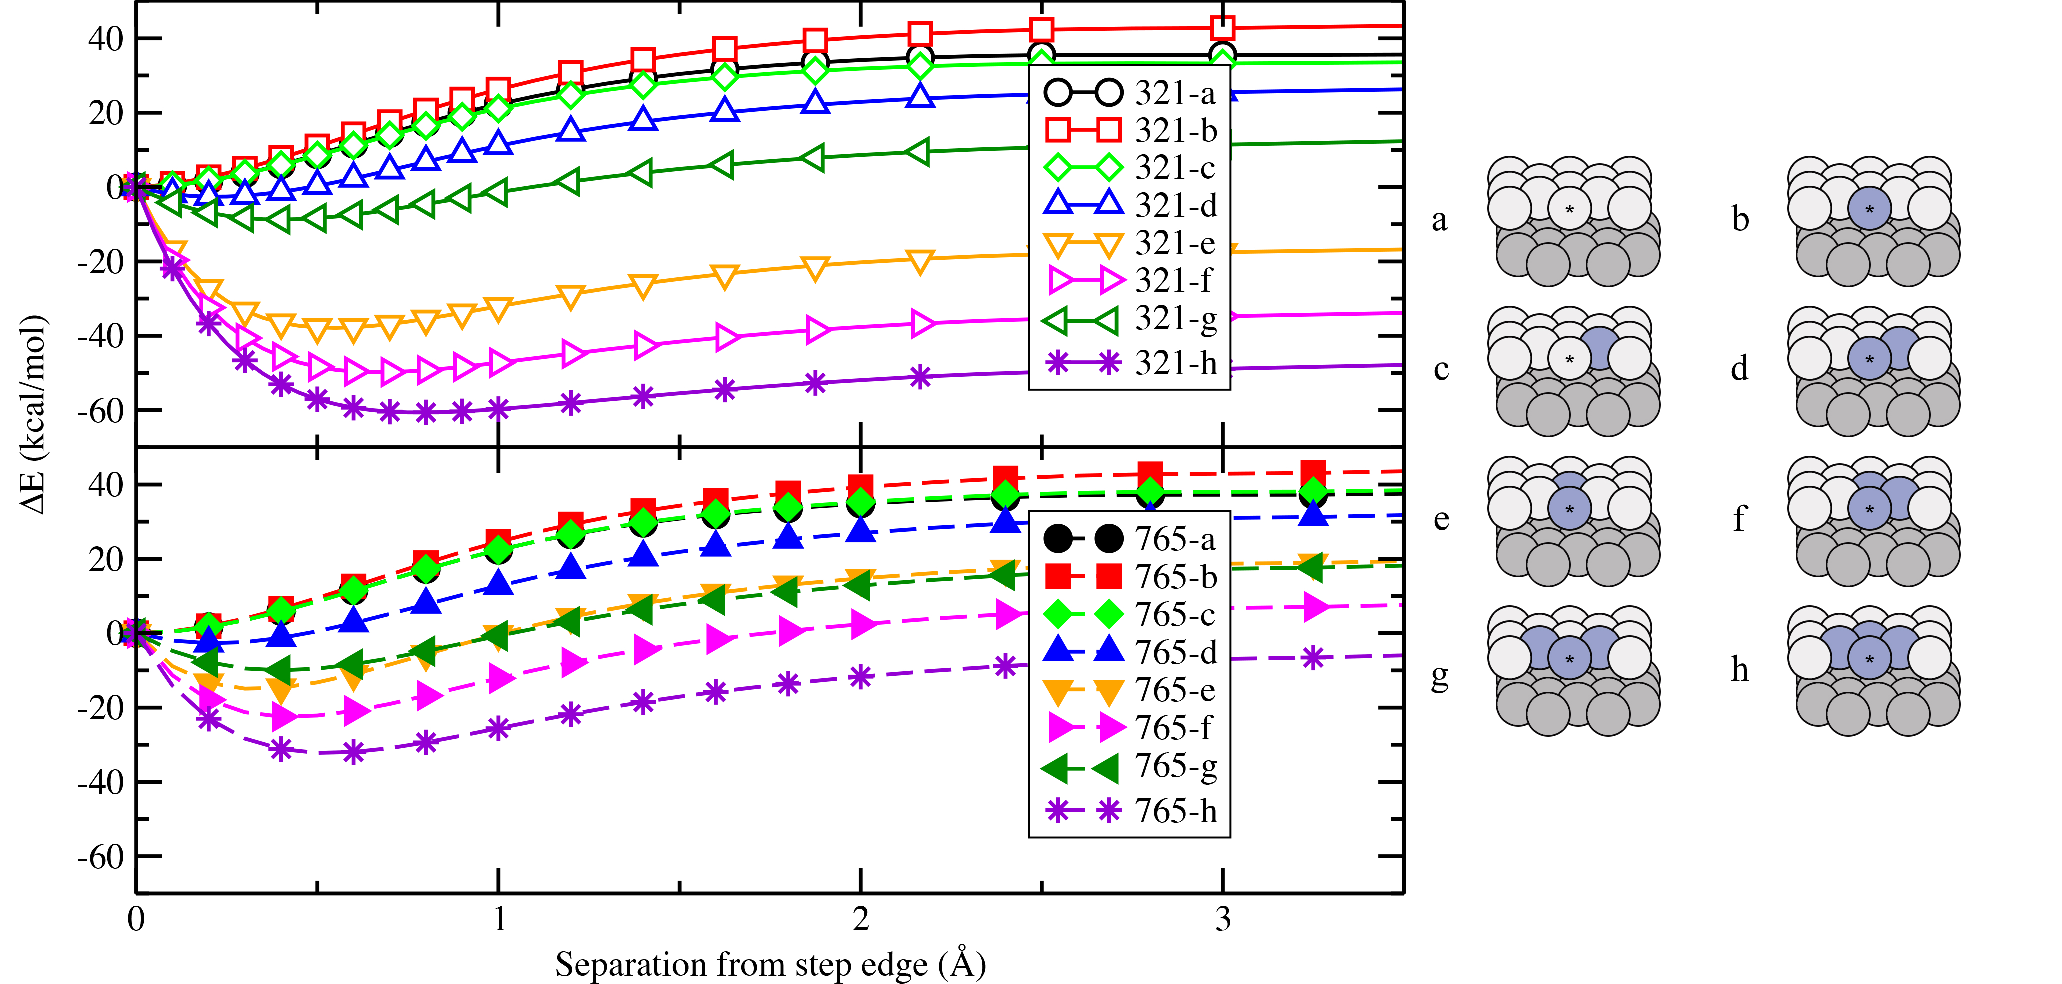
\includegraphics[width=0.75\linewidth]{../figures/chap4/321_765_EnergySeparation.pdf}
  \caption{Similar to Figure \ref{fig:112_557_ES}, these graphs depict the
energies for displacing an edge atom perpendicularly from either the (321) or
(765) step edges. The configurations to the right of the graphs represent the
rougher kinked step edges of these facets. The rougher steps lower the 
energetic barrier for adatom creation when compared to the flat steps of the
(112) and (557) surfaces.}
\label{fig:321_765_ES}
\end{figure}
\end{landscape}

In general, this analysis provides several helpful results. First, removing an
atom from a (321) or (765) step is more energetically favorable than from a
(112) or (557) step. This is due to the lower coordination of atoms in
the kinked edges. This trend is clearly shown in Figures \ref{fig:112_557_ES}
and \ref{fig:321_765_ES} for configuration a where no CO is present on the
surface. In these instances, removing an atom from a kinked step edge is 10
kcal/mol more favorable than it is to form an adatom from a flat step. This is
directly due to the lower coordination of the atoms in the kink steps.
Second, the length of the plateau seems to also affect the energy required to form
an adatom at higher coverages.  Configurations e, f, and h in Figure
\ref{fig:321_765_ES} for the kinked steps highlights this result well. It is
approximately 25 kcal/mol more favorable to form an adatom on the (321) surface
than it is on the (765) surface. Similarly, there is approximately a 20
kcal/mol difference in favor of forming  forming an adatom from a (112) step-edge when
compared to the (557) surface.

Finally, the location and arrangement of \ce{CO} also strongly affects the
required energy to remove the atom from the step edge. Separation becomes most
favorable when the atom that is becoming the adatom and the atom directly
behind it both have an adsorbed \ce{CO}. This configuration directs the strong
quadrupolar repulsive force directly away from the step edge, thus lowering the
energetic barrier for adatom formation.  This conclusion can be demonstrated by
comparing configurations d and e in both figures. In configuration e, the
\ce{CO} are located along a vector which is aimed perpendicularly away from the
step, while in configuration d the repulsive force generated by the \ce{CO} is
either completely or mostly parallel to the step edge. As the coverage
increases, the likelihood of a higher energy configuration also increases,
which leads to more step-edge breakup and a larger surface diffusion.

\subsubsection{Straight vs. Kinked edges}
As highlighted in Figure \ref{fig:diamonds}, one of the partial reconstructions
observed on the (321) surface are the small diamonds composed of (111) domains
formed between steps. Most of these diamonds share corners corresponding to
nucleation sites between steps from which zippering into double steps is
observed primarily on the 0.5 ML surfaces. The initial formation of these
diamonds however is of fairly low cost. Principally, the hopping
diagrammed in Figure \ref{fig:kinkSketch} has a barrier of approximately ?
kcal/mole while the resulting structure is within 0.1 kcal/mole of the original
surface. While the presence of \ce{CO} provides some of the driving force for
this hopping, the resultant increase in (111) domain size on the surface
combined with the numerous nucleation sites that are formed between steps leads
to this patterning existing as a metastable state in many of our simulations of
the (321) surface. In contrast, the straight steps on the (112) and (557)
surfaces, while sources for adatoms, did not provide any benefit to doubling.

\begin{figure}
  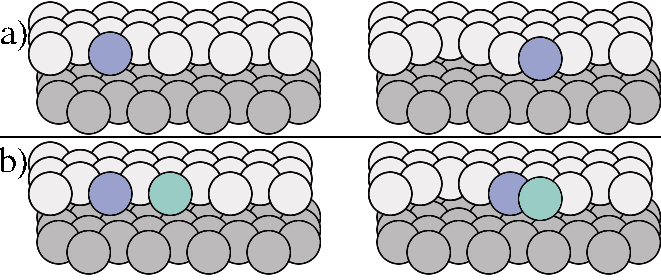
\includegraphics[width=\linewidth]{../figures/chap4/kinkMovement.pdf}
  \caption{Models of the ``kinked'' edge features of the (321) and (765)
surfaces.  One of the most commonly observed adatom movements on the surface
involves one of the kink atoms hopping to a nearby edge binding site. This is
predicted to happen in one of two ways, (a) the highlighted blue atom is
ejected and traverses in a curvilinear path to its end point or (b) the blue
atom dislocates the green atom resulting in the same final configuration. The
formation of longer (100) segments of the step-edge slightly lowers the surface
energy leading to a more stable surface.}
  \label{fig:kinkSketch}
\end{figure}

\subsection{CO binding energy}
%Coverage, temperature of system (compare to original data?)
The decrease in the parameterized \ce{Pt\bond{-}CO} interaction was made in
response to recent DFT results\citep{Deshlahra:2012aa} and uncertainties about
previously reported calorimetric heats of adsorption for the \ce{Pt\bond{-}CO}
interaction.\citep{Yeo:1997th} As the decrease in this binding energy results
in fewer CO being adsorbed at any given instant in the simulations, this also
leads to a decrease in adatom generation and concomitantly a decrease in
step-edge wandering. For the surfaces that had short plateaus, this decrease
did not appear to affect the doubling as the edges did not have to wander as
far to still meet, but for the (557) and (765) surfaces,  doubling was not
observed for this parameter set.

\subsection{Mechanisms of structural changes}
Our previous work on \ce{Pt} (557) revealed that the presence of \ce{CO} initially
destabilizes the step-edges leading to rapid formation of adatoms and
step-wandering on the surface. If significant step-wandering occurs such that
two edges connect, they often form a ``nucleation'' site, a location that
connects two step edges and is stable for a significant portion of time. Once
one of these sites is formed, step-wandering will often lead to ``zippering''
of the two edges into a double step. 

This mechanism initially depends on the stochastic meeting of two step edges
which is well-correlated with the density of adatom formation. Increased
thermal energy is one method to increase the number of adatoms on stepped
surfaces, however is these simulations we attempted to limit this through
lowered simulation temperatures.  The presence of \ce{CO} is playing a similar
role to an increased temperature by weakening the \ce{Pt\bond{-}Pt} bonds in
the step-edge.

The density of adatoms is one factor in determining the likelihood of step-edge
meeting, while the other primary factor is that of plateau length. The (112)
and (321) systems have shorter plateau lengths which makes the chance of
step-edges meeting more likely.  In our previous work on the (557) surface,
only one nucleation site formed per observed step-edge doubling, for some of
the systems explored in this study, numerous nucleation sites were created
before the steps could finish doubling, which in some cases led to partially
doubled step edges, highlighted in Figure \ref{fig:partialDoubleLayer}.

Further evidence of the importance of plateau length was elucidated from the
observed differences between the different (321) systems. The
longer steps tended to have more partially formed double layers as
a result of numerous nucleation sites. This prevented the full
zippering mechanism from occurring. In contrast, the (321) steps that were
extended to display a greater number of steps had a few
instances of complete step edge doubling.

All surfaces, even those without \ce{CO} present showed some amount of surface
roughening and reconstruction suggesting that the surface is only quasi-stable
at high temperatures. However, the presence of \ce{CO} at 0.25 and 0.5 ML
coverages did lead to significantly more step-wandering intermediate
reconstructions and partial and full double layer formation.

%Dynamics of GCN for surfaces


%The slight refaceting of the surfaces led to an artificially low diffusion
%constant for these systems (true?) because the majority of steps have become
%slightly buried in these systems to reduce the high surface energy of these
%systems. Nevertheless, the remaining (100) steps were large sources of adatoms
%which was increased as \ce{CO} coverage was also increased. If the system were
%kept at an elevated pressure and prevented from relaxing along the
%step-direction, it is likely that the (100) steps would be better maintained
%and a larger amount of surface movement and eventual doubling would be
%observed.

\section{Summary}
The mechanism of reconstructions on \ce{Pt} surfaces, specifically step-edge
doubling, is dependent on the displayed surface facet. It is also
partially dependent on the presence of adsorbates, here \ce{CO}, that can 
disrupt the step-edges and then stabilize the formation of double steps. An in-depth
examination of the energetics of step-edge breakup shows that the ``kinked''
surfaces (321) and (765) are especially favorable for formation of adatoms
because of the under-coordination of the kinked edge atoms. The stochastic
mechanism proposed in earlier work which stated that the meeting up of two
edges was ultimately a stochastic process and then double layer formation would
typically proceed in a ``zippering'' fashion is strengthened here as a number of
systems with shorter plateaus ended up in frustrated double layer formations.

The lack of any double steps forming on the (557) surface despite being seen in
an earlier set of simulations suggests that the re-parameterization of the
\ce{Pt\bond{-}CO} interaction to better match reported experimental values has
altered the dynamics of the step-doubling process.  While significant
step-wandering was still observed on these systems, the density of adatoms was
not sufficient to stochastically form a nucleation site during the simulation
time.

Recent work on \ce{CO}-induced nanostructure formation on a \ce{Cu} (111) has
shown that when the metal-metal binding interactions are weaker, the presence
of strong repulsive adsorbates can be sufficient to disrupt even flat
surfaces.\citep{Eren:2016qt} We have reached a similar conclusion with the
\ce{Pt} systems explored for this investigation, such that surfaces that have a
higher surface energy and more sites where adatoms can be easily formed, ({\em
i.e.} weakly-bonded atoms) are more likely to experience reconstruction in
general and doubling of the step-edges specifically as this greatly increases
the amount of the surface that is occupied by the more stable (111) domains.




\chapter{DEVELOPMENT OF A MULTIPLE-MINIMA FLUCTUATING CHARGE (MM-FLUCQ) POTENTIAL FOR PLATINUM-OXIDE FORMATION}
\label{chap:mmFlucQ}


In this chapter a brief overview of charge transfer methods will be presented
alongside the initial development of the mm-FlucQ potential.  Preliminary
results of charged species approaching a \ce{Pt} surface will also be
examined. Finally, current challenges and future directions will be discussed.

%polarization near metal surfaces
% drude model
% charge transfer

\section{Introduction}
Metal surfaces and interfaces play a key role in a number of chemical and
technological processes; however, the tendency of oxide layers to form on these
interfaces requires a chemically-realistic treatment of metal-adsorbate
interactions when simulating these systems\citep{Streitz:1994mw, Duin:2010dk,
Devine:2011bk, Fantauzzi:2014pb}.  The modified atomistic structure and
electronic environment of these surfaces after oxide formation is expected to
affect many properties of the interface, especially the local electric field,
the polarization of the surface, and also diffusion and adsorption on the
surface.\citep{Streitz:1994mw, Getman:2008sp, Bray:2011hq,Small:2012dw}

There have been numerous attempts to include charge transfer and polarization
within molecular simulations.\citep{Rick:1994ss, Streitz:1994mw,
Siepmann:1995es, Iori:2008ic, Iori:2009au} Depending on whether atomic or
molecular polarizability is desired, different implementations are more or less
appropriate. The polarization of molecules and metals is often treated using
various charge transfer methods, whereas atomic polarizability is typically
reliant on a dynamic multipole representation of the charge density of the
atom.

One of the simplest ways to include atomic polarizability is with the use of
Drude particles, which are loosely based on Drude's model electrical
conductionthat he proposed in 1900.\citep{Drude:1900aa, Drude:1900bb}. In the
description of these particles, the static charge of atom $i$ is decomposed
into two portions, generally a larger portion that is retained at the atomic
location, and the remaining portion that is allowed to move ``freely'' around
the atomic site, typically constrained by either a fixed distance $r$ or a
standard restoring force with an equilibrium distance of $r_e$. If the atom is
neutral, the creation of a small dipole moment by placing a positive charge at
the atomic site and a negative charge at the end of the rod or spring can lead
to an effective treatment of the anisotropic atomic polarization. This method
can be expanded to molecular systems and has been used by Roux {\em et al.} to
describe a simple polarizable model for water.\citep{Roux:2003ho}

A further modified version of this method has been recently utilized by Iori
and Corni in their modeling of biological adsorption on gold
surfaces.\citep{Iori:2008ic, Iori:2009au} Each gold atom was assigned a small
negative charge which was balanced with an equally small positive charge a
short distance away. When there were no perturbations present, the system
dipole averaged to zero, but when charged adsorbates approached the surface, a
net dipole moment was formed in response.

Polarization can also be included by incorporating charge transfer into the
description of the system. While atomic level polarizability is not inherently
present in this approach, for larger molecular systems, allowing
intramolecular charge transfer can still capture a significant amount of
observed polarization. Rick, Stuart, and Berne, in their fluctuating charge
model of water made use of intra- and inter-molecular charge transfer to more
accurately describe condensed phase properties of water.\citep{Rick:1994ss} One of the
strengths of their approach was their treatment of atomic charge as a dynamical
variable that would gain and lose velocity as a result of the local electronic
environment. This allowed them to avoid large matrix calculations every time
step, which had been used previously to ensure a charge minimum in simulated
molecular systems. 

A similar approach, but expanded to describe metals was proposed by Siepmann
and Sprik where they described the charge on a metal as a gaussian density
where the charge variables were again included in an extended lagrangian so
that a constraint on the surface potential could be
enforced.\citep{Siepmann:1995es} This restriction on the potential led to an
accurate capturing of the image charge formalism often used in continuum
electrostatics. Their investigation of water ordering on metal surfaces did not
include any charge transfer between the water and the metal. Instead they
described the primary interactions between the metal surface and the water
molecules with a generalized interaction potential shown below,

\begin{equation}
\nu_2(r_{ij}) = \frac{A}{r_{ij}^\alpha} - \frac{C}{r_{ij}^6} - \frac{Df_2(r_{ij})}{r_{ij}^3}\Phi_{ij}(\phi_{ij})
\end{equation}

where, $A, C, D, $ and $\alpha$ are tunable parameters. The first term captures
the isotropic soft-core repulsion, while the second term on the right captures
the disperion attraction. The third term is composed of a cutoff, $f_2(r) =
e^{\frac{B}{r-r_{\mathrm{cut}}}}$, and angle dependent piece based on the
Stillinger-Weber model\citep{Stillinger:1985tb} which helps capture some of the
chemical binding that leads to an atop-preference.

Treating the charge transfer dynamics of any of the above systems within
molecular dynamics is a challenging problem and while non-metallic species can
be modeled satisfactorily with static point charges, metal-adsorbate, metal
oxide, and more generally metal-metal interactions require a more complicated
description of their electronic interactions to accurately capture the behavior
of charged species near a conductor. One helpful idea that has been of great
use in implementing charge transfer schemes is that of electronegativity
equalization. Introduced by Sanderson\citep{Sanderson:1951mz},
electronegativity equalization provides a conceptual framework that describes
charge transfer between both atomic and molecular species. In this formalism,
as a species gains negative charge in response to its local environment, its
electronegativity decreases; similarly, if an atomic site has lost charge, then
it has an increased electronegativity. The system would then only be considered
at equilibrium if all of the electronegativities were equal.  It is helpful to
remember that the electronegativity, $\chi_A$, as defined by
Mulliken\citep{Mulliken:1934wt} is equal to the negative of the chemical
potential of the valence electron gas around a positive nucleus, $\mu_A$, as
argued by Iczkowski and Margrave\citep{Iczkowski:1961wq}.

\begin{equation}
\chi_A = -\mu_A = -\frac{\partial E}{\partial q}
\end{equation}

In this equation $E$ is the ground state energy of the atom while $q$, the net
charge of the atom, is equal to $n - Z$ where $Z$ is the atomic number and $n$
is the number of electrons around the nucleus. Thus $q = 0$ for the neutral
species, $+1$ for the positive ion, and $-1$ for the negative ion.  This
description implies that upon movement of the nuclei, the electrons will
undergo charge transfer so as to equilibrate the electrochemical potential of
the system. While this formalism is helpful, it still requires a method of
implementation.  Streitz and Mintmire, using the idea of electronegativity
equalization, developed a potential for modeling aluminum oxide. They
calculated the minimum charges at each time step by taking the inverse of an
$n\times n$ matrix, which while accurate, drastically increases the expense of
a simulation.\citep{Streitz:1994mw} A method proposed by Rick {\it et al.} in
their work on fluctuating charge water models is able to avoid matrix inversion
by allowing the atomic charges to fluctuate dynamically. This was accomplished
by coupling the electronegativity equalization method with a fictitious charge
variable on each atomic site. This charge variable $Q_A$ was then propagated
with the rest of the dynamics of the system by using an extended Lagrangian
approach.\citep{Rick:1994ss}

The basic idea of a dynamic fluctuating charge model is to allow partial
charges on atomic sites to become dynamical variables.  Each atomic site
therefore has four ``position'' variables, $\{\vec{\mathbf{r}}_A, Q_A\}$, and
four velocities, $\{\dot{\vec{\mathbf{r}}}_A, \dot{Q}_A\}$.   In addition to
standard electrostatic interactions between the fluctuating charges, there is a
self energy term that must be taken into account. Similar to Rapp\'e and
Goddard\citep{Rappe:1991dq} we can make use of a Taylor expansion around the
neutral atomic species with respect to charge.  This self term through second
order leads to,

\begin{equation} \label{eqn:selfenergy}
E_A(Q_A) = E_{A_0} + Q_A\bigg( \frac{\partial E}{\partial Q} \bigg )_{A_0} +
\frac{1}{2}Q_A^2 \bigg(\frac{\partial^2E}{\partial Q^2}\bigg)_{A_0}
\end{equation}

where $E_{A_0}$ is the ground state energy of the neutral species, $A$, and the
higher order terms are shown to be the electronegativity, $\chi$, and
electronic hardness, $J$, as derived below,

\begin{align*}
\mathrm{IP} &= E_A(+1) - E_A(0) \\
& = E_{A_0} + \bigg (\frac{\partial E}{\partial Q}\bigg)_{A_0} + \frac{1}{2}\bigg(\frac{\partial^2E}{\partial Q^2}\bigg)_{A_0} - E_{A_0} \\
\mathrm{EA} &= E_A(0) - E_A(-1) \\
& = E_{A_0} - E_{A_0} + \bigg (\frac{\partial E}{\partial Q}\bigg)_{A_0} - \frac{1}{2}\bigg(\frac{\partial^2E}{\partial Q^2}\bigg)_{A_0}  \\
\bigg (\frac{\partial E}{\partial Q}\bigg)_{A_0} &= \frac{\mathrm{IP+EA}}{2} = \chi_A ,\qquad \bigg (\frac{\partial^2 E}{\partial Q^2}\bigg)_{A_0} = \mathrm{IP-EA} = J_A
\end{align*}

where IP is the ionization potential and EA is the electron affinity of species
$A$.  Note that this approach assumes the surface is smooth in the
$+1 \rightarrow -1$ charge domain. This description allows us to rewrite equation
\ref{eqn:selfenergy} as the following,

\begin{equation}
E_A(Q_A) = E_{A_0} + \chi_A Q_A + \frac{1}{2} J_{A} Q_A^2
\label{eq:harmonic}
\end{equation}

The electronegativity $\chi$, when described as the average of the ionization
potential and electron affinity, enjoys some agreement with experimentally-derived properties; whereas a
definition of electronic hardness is best understood using Rapp\'e and
Goddard's approach, where $J$ is equal to the Coulomb overlap integral between
Slater orbitals centered on each atomic site\citep{Rappe:1991dq}.

The harmonic self energy, shown in equation \ref{eq:harmonic} is enormously useful.
Even in large systems of coupled fluctuating charge sites, the charges move on
a purely harmonic ``bowl'' where the minimum energy state for the system of
charges can be determined uniquely. Charge conservation constraints can be
applied to a constrained electronegativity equalization procedure to find the
best set of charges for a given set of nuclear positions.  Additionally, motion
of the atomic sites simply changes the location of the minimum and curvature of
the charge bowl, but these are relatively smooth variations, allowing standard
integration techniques to be used to propagate the charge variables.

One limitation of the harmonic self-interaction potential is the inability to
represent multiple stable oxidation states of various species. In many simple
molecules or ions, only one dominant oxidation state is present, but at the
surfaces of metals (and particularly during metal oxide formation), there can
be multiple oxidation states (e.g. \ce{Pt^0}, \ce{Pt^2+}, \ce{Pt^4+}, etc.)
present in the system simultaneously.

Another weakness of the harmonic approach is the reliance on the unit charge
gas phase ions in determining the first and second derivative terms, $\chi$ and
$J$.  In many charge partitioning schemes (and in most classical force fields),
the partial charges assigned to condensed phase atoms are significantly smaller
than the unit charges required to produce the gas phase ions, e.g. the \ce{H}
in \ce{H2O} in TIP4P is assigned a charge of +0.52.\citep{Jorgensen:1983tp}
This results in electronegativity and hardness terms that may estimate the
local slope and harmonic constants leading to construction of a charge surface
that is overly broad.

The method we present here builds on the fluctuating charge method of Rick {\it
et al.}\citep{Rick:1994ss}, but models the self energy more generally using
multiple stable ionic states.  This multiple-minimum fluctuating charge method
(mm-FlucQ) effectively allows for charge transfer between ionic and metallic
species.

\section{Development of methodology}

As we present the development of this approach, it is helpful to see how it
will fit into the total Lagrangian of the system. Similar to Rick {\it et
al.}\citep{Rick:1994ss} our Lagrangian is shown below,

\begin{equation}
L = \sum^{N_{molec}}_{i=1}\sum^{N_{atom}}_{\alpha = 1} \frac{1}{2}m_{\alpha} \dot{r}^2_{i\alpha} + \sum^{N_{molec}}_{i=1}\sum^{N_{atom}}_{\alpha = 1} \frac{1}{2}M_Q\dot{Q}^2_{i\alpha} - U[(\mathbf{Q}),(\mathbf{r})] - \lambda \sum^{N_{molec}}_{i=1}\sum^{N_{atom}}_{\alpha = 1} Q_{i\alpha}
\end{equation}

where the mass of an atomic site $\alpha$ is defined as $m_\alpha$ and $M_Q$ is
the fictitious charge mass with units of $\frac{\mathrm{energy\times
time}^2}{\mathrm{charge}^2}$.  The $\lambda$ term at the end of the Lagrangian
allows us to enforce total charge conservation in the system.

The potential energy term $U[(\mathbf{Q}),(\vec{\mathbf{r}})]$ contains the
expected pieces from standard molecular dynamics simulations,
$U_{\text{bonds}}, U_{\text{bends}}, U_{\text{torsions}},
U_{\text{electrostatics}}, U_{\text{van der Waals}}$ etc. It also contains the
new self energy term necessary for modeling dynamic fluctuating charges. This
term, instead of using the harmonic approximation, includes multiple diabatic
charge states,

\begin{equation}
U(Q) =
\begin{Bmatrix}
 V_0(Q) & c  \\
 c   & V_1(Q)
\end{Bmatrix}
\end{equation}

Where $c$ is a coupling constant between states $i$ and $j$, and $V_i(Q)$ is
seen below,

\begin{equation*}
V_i(Q) = \frac{1}{2}k(Q - Q_i)^2 + V_i
\end{equation*}

For each diabatic state, $V_i(Q)$ treats the local energy around a stable charge
site, $Q_i$, as a harmonic function with local curvature $k$ and offset by $V_i$.
By constructing our self-potential energy landscape out of many
diabatic states, we are able to create a surface with multiple charge minima.
An ideal multiple-well potential is shown in Figure \ref{fig:multipleDiabat}.
This method can be trivially extended by adding more diabatic states.

\begin{figure}
  \centering
  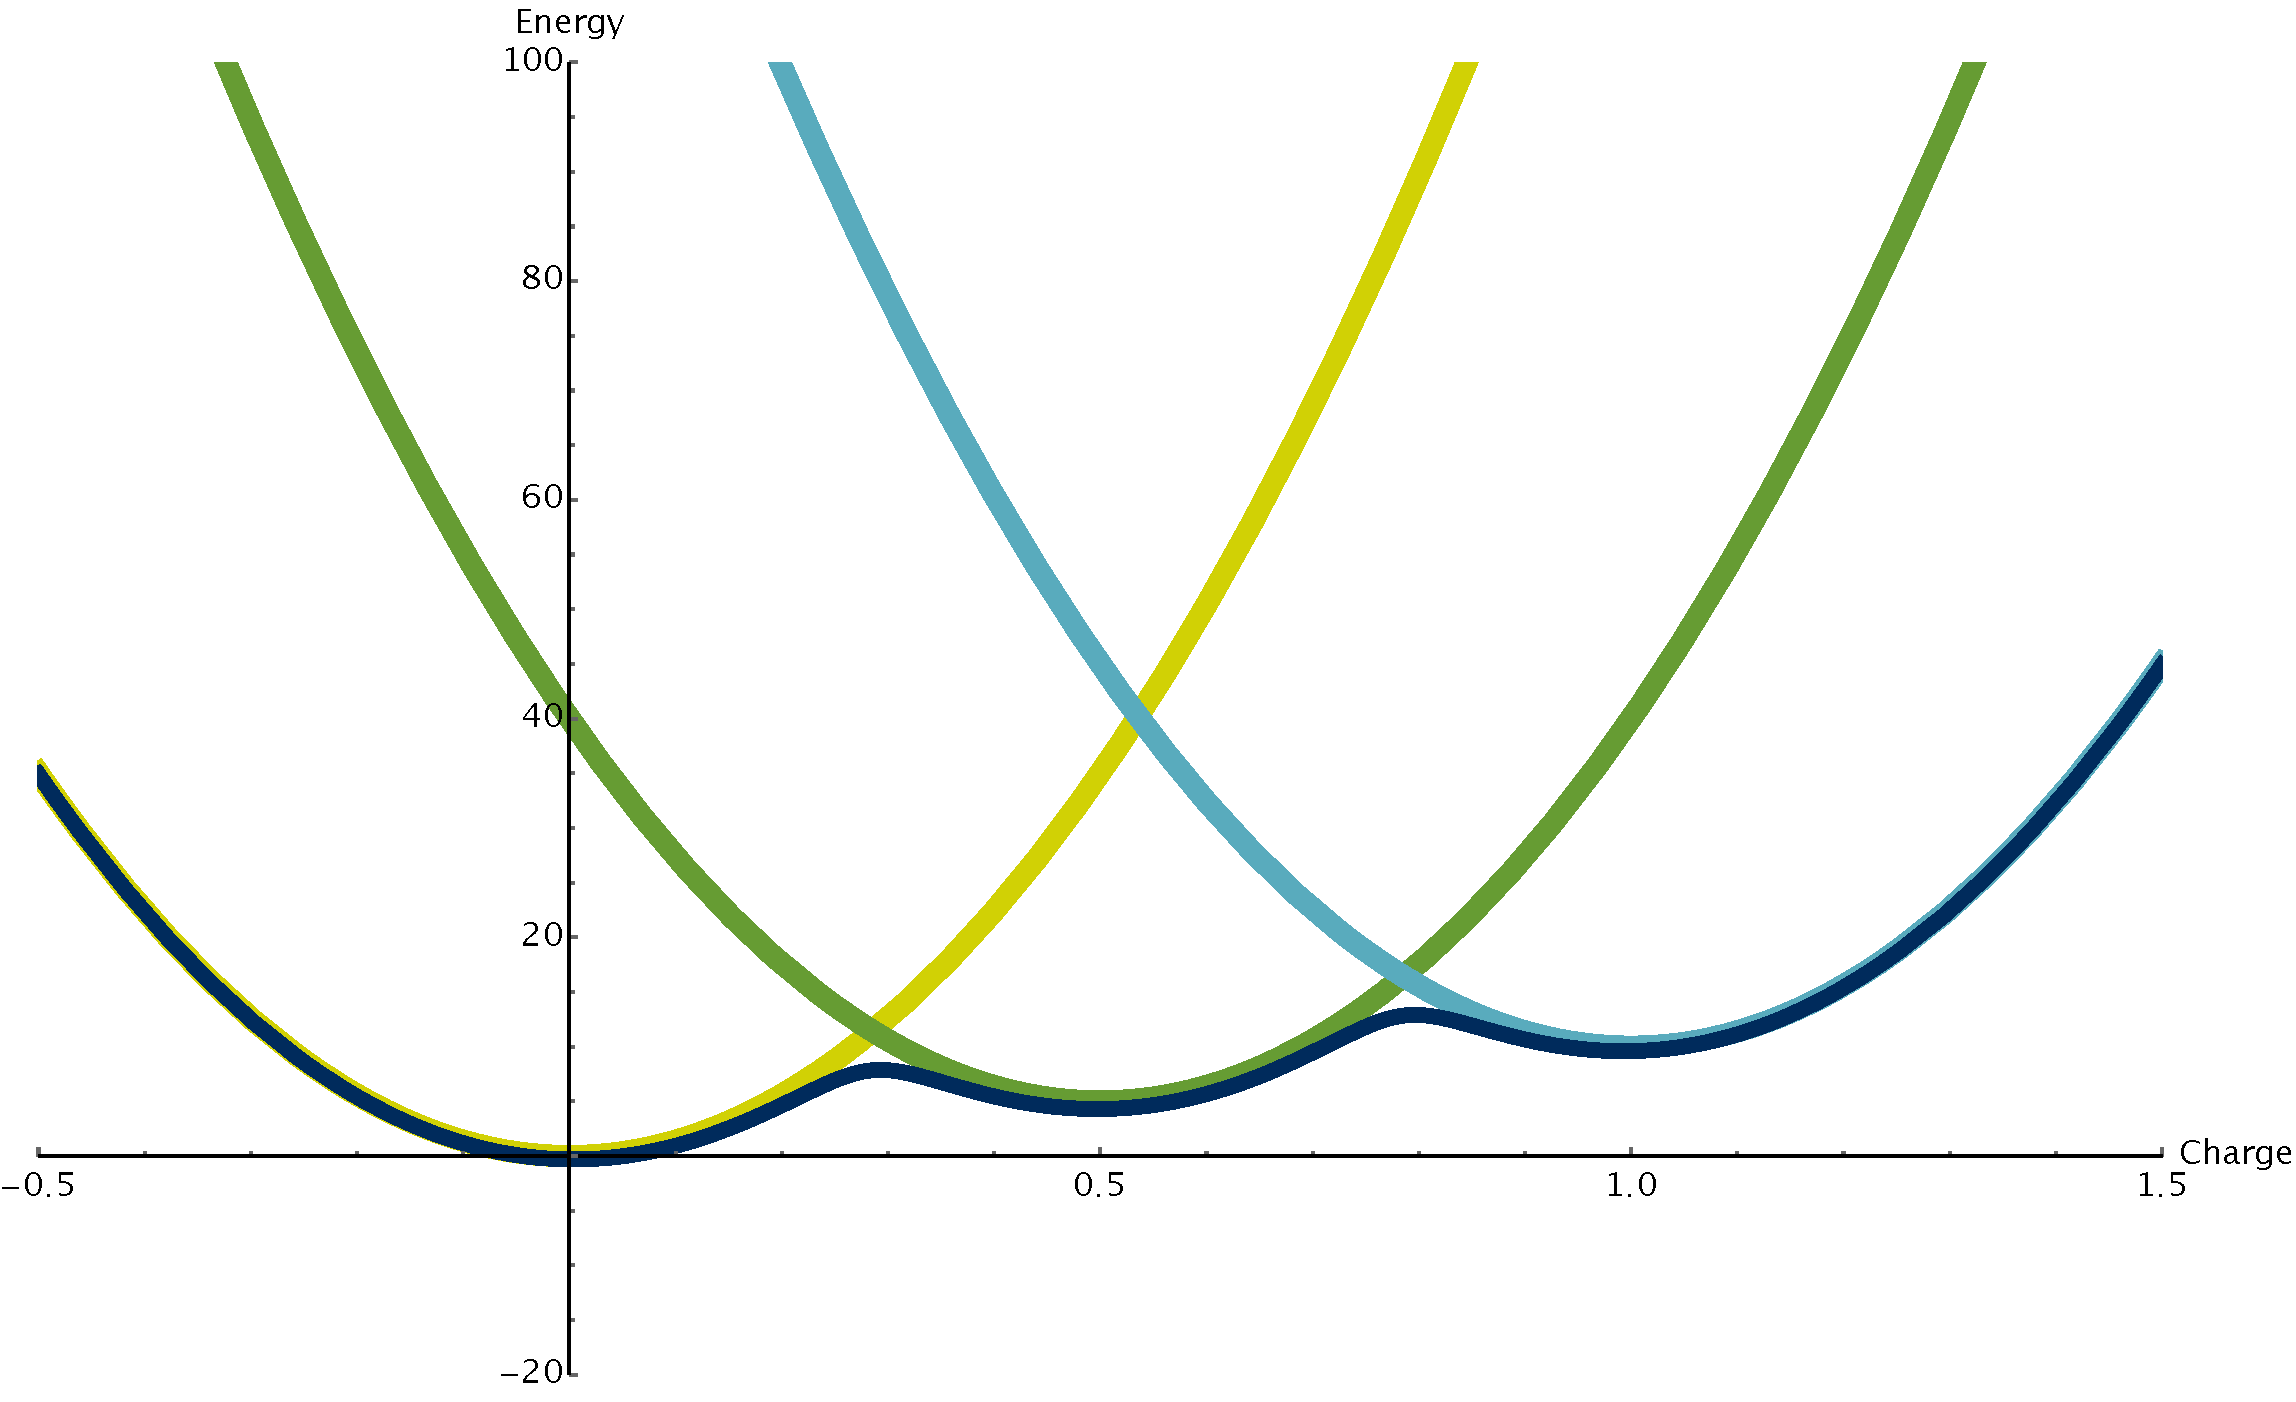
\includegraphics[width=0.75\linewidth]{../figures/chap5/multipleDiabats.pdf}
  \caption{The gold, green, and cyan curves represent the diabatic energies
that compose the navy triple-well adiabatic potential surface which is defined
using the following parameters and solving for the eigenvalues of the matrix.
$[Q_0 = 0, Q_1 = 0.5, Q_2 = 1, V_0 = 0, V_1 = 5, V_2 = 10, k = 280, c = 3.5]$}
\label{fig:multipleDiabat}
\end{figure}

\begin{equation*}
  \begin{Bmatrix}
    V_0(Q) & c      & 0      & \dots  & 0\\
    c      & V_1(Q) & c      & \dots & 0\\
    0      & c      & V_2(Q) & \ddots & 0 \\
    \vdots & \vdots & \ddots & \ddots & c\\
    0      & 0      & 0      &  c     & V_n(Q) \\
    \end{Bmatrix}
\end{equation*}

\subsection{Parameterization}
One weakness of this proposed method is the need for a large number of
parameters.  Currently, even with assumptions made about a single coupling
constant $c$, no coupling between states when $|i-j| > 1$, and $k$ being the
same for all of the individual diabatic states, there will still need to be
$2n+2$ parameters for $n$ diabatic states. 


\subsubsection{Platinum \& Oxygen self-potentials}
A more complicated example is the electronic surfaces
of oxygen and platinum in a platinum-oxide system.  The ``stable'' charge minima of the diabatic wells
were obtained from a set of DFT calculations performed on
the platinum oxide surface. Bader charge analysis was performed and a histogram
was generated based on the populations of oxygen and platinum in various charge
states. The population analysis of both species is shown in Figure
\ref{fig:population} and a first attempt at the interaction potentials were
then created and are shown in Figures \ref{fig:Ocharge} and \ref{fig:PtCharge}.
The current approach attempts to minimize the effects of the bulk \ce{Pt} when
determining relative barrier heights between charge states.

\begin{figure}
  \centering
  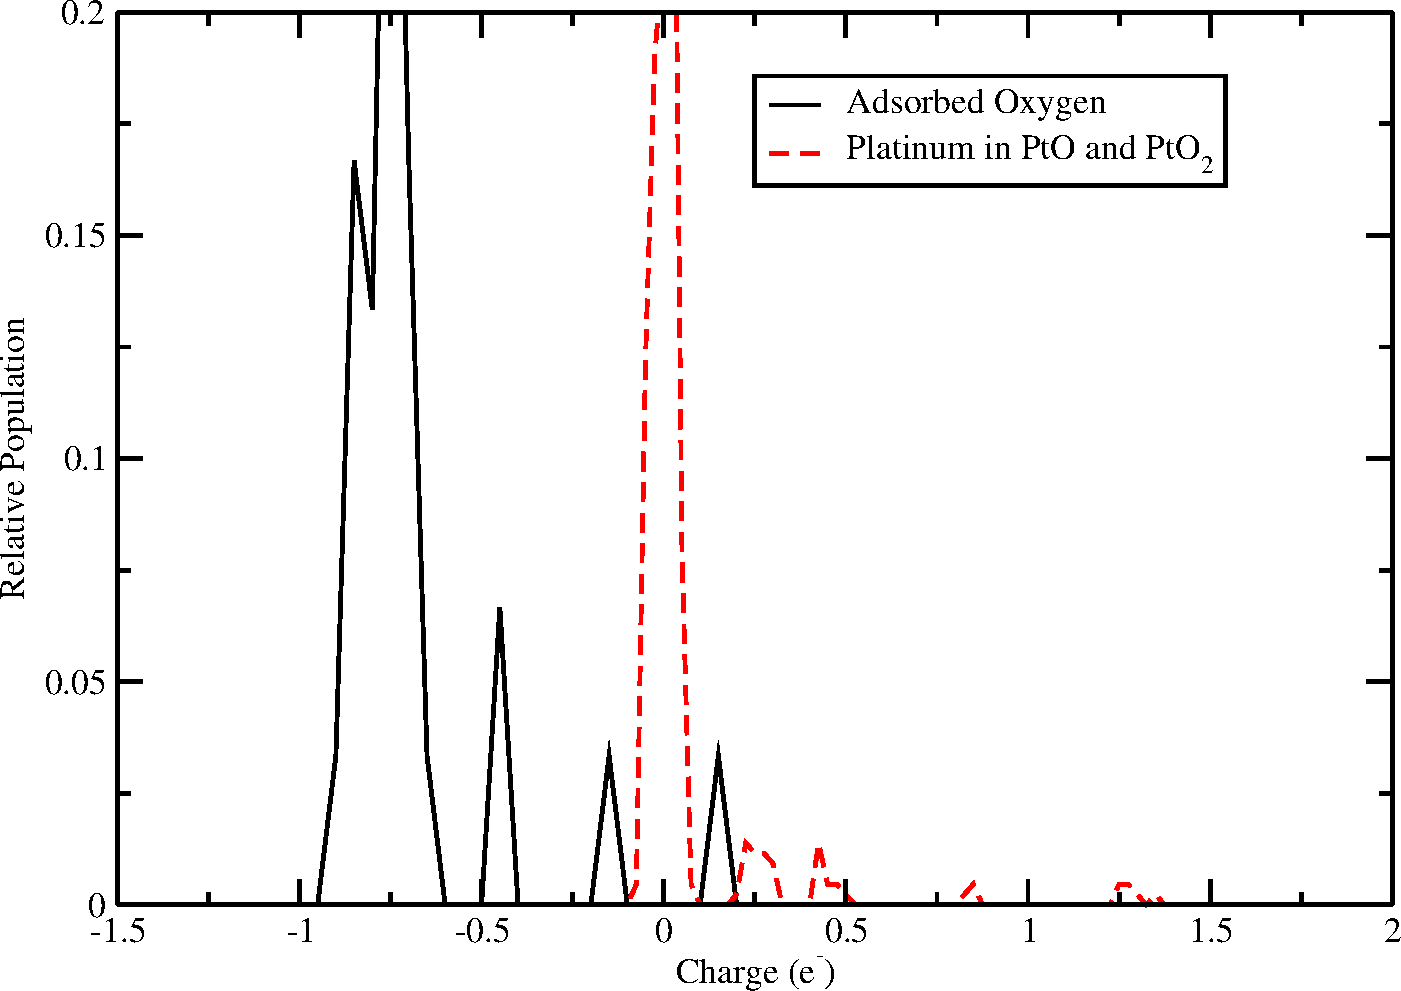
\includegraphics[width=0.75\linewidth]{../figures/chap5/chgDist_PtO.pdf}
  \caption{Histogram of oxygen (black, solid) and platinum (red, dashed)
charges obtained from a sampling of platinum oxide DFT calculations.
Normalization is proportional to the number of atoms in the simulation, hence the
large peak centered around 0 for \ce{Pt}, since the majority of the metal is
unperturbed by surface \ce{O}.}
\label{fig:population}
\end{figure}

\begin{figure}
  \centering
  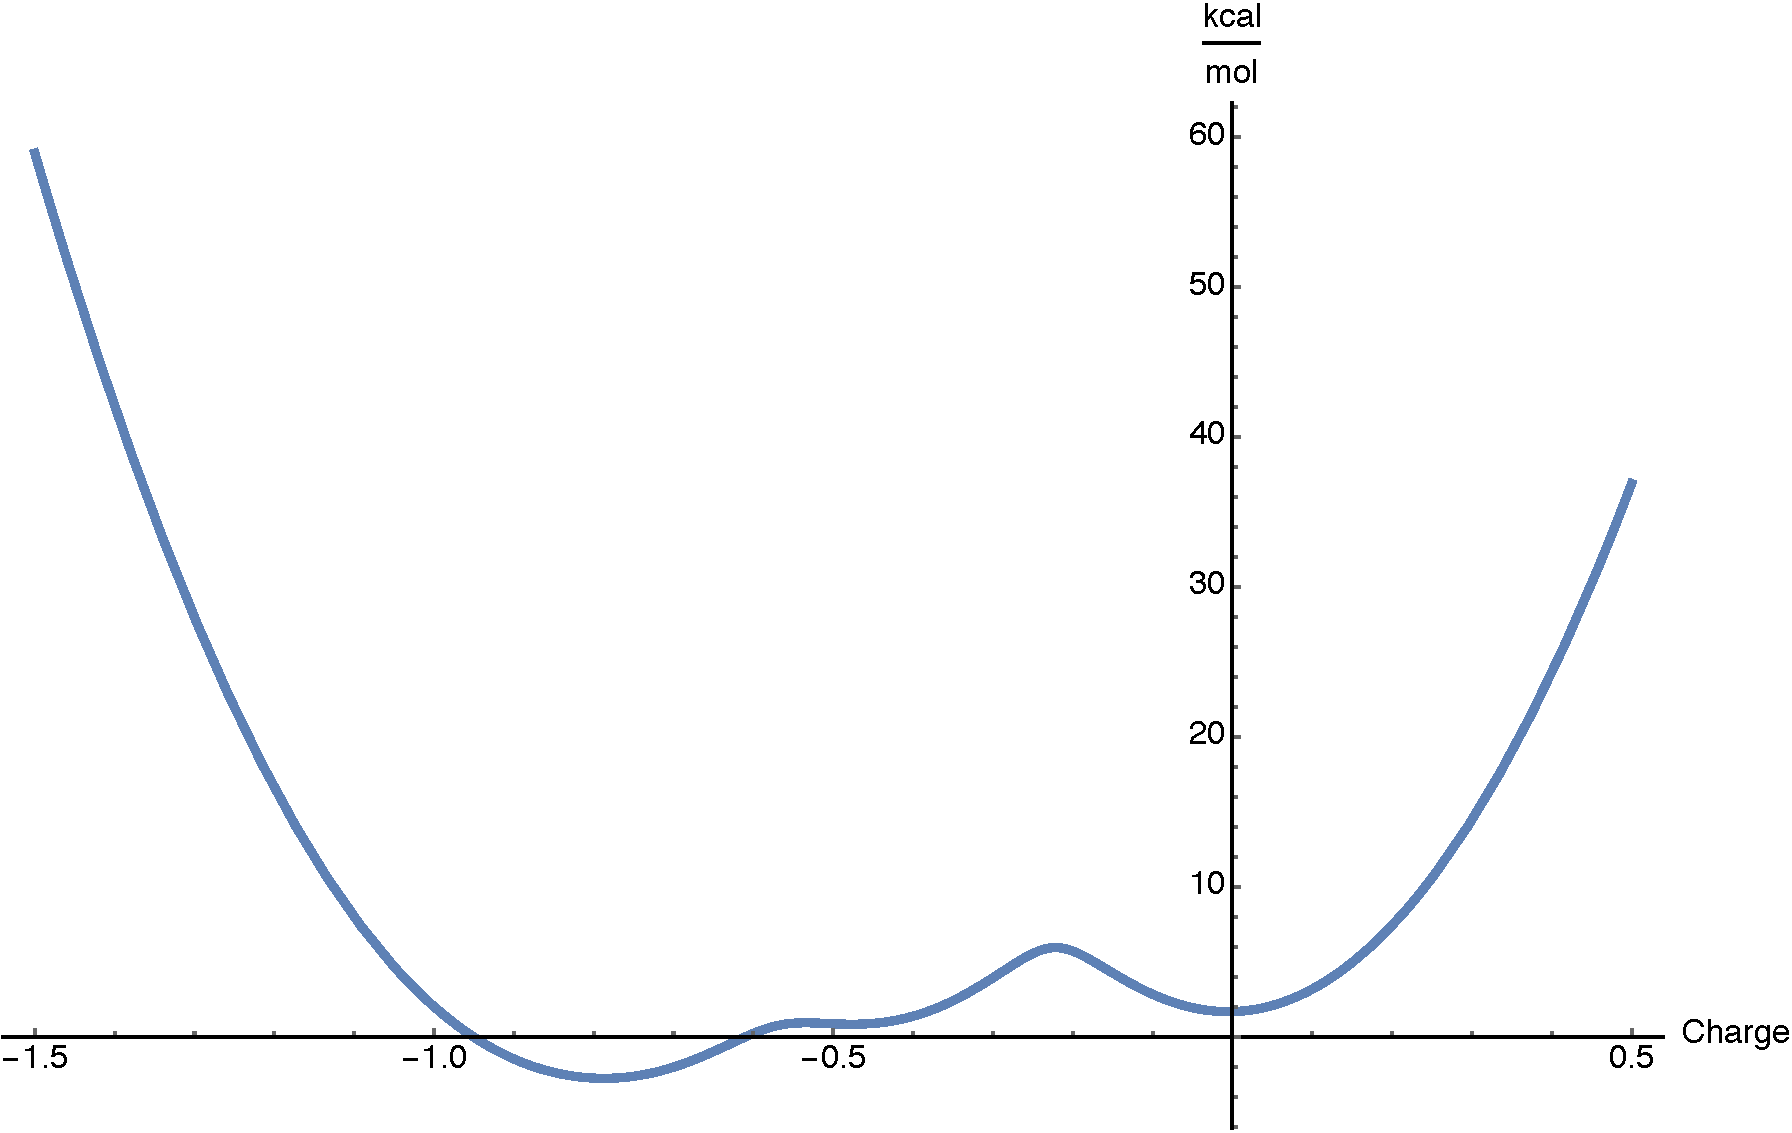
\includegraphics[width=0.75\linewidth]{../figures/chap5/Oxygen_Charge_Testing.pdf}
  \caption{The self-interaction oxygen potential. The parameters to
generate this potential are $[Q_0 = -0.85, Q_1 = -0.75, Q_2 = -0.45, Q_3 = 0,
V_0 = 0.25, V_1 = 0, V_2 = 2, V_3 = 2, k = 280, c = 3]$. As oxygen has a
favorable first electron affinity, it was decided that the global minimum
would be located around that point in this fit.}
\label{fig:Ocharge}
\end{figure}

\begin{figure}
  \centering
  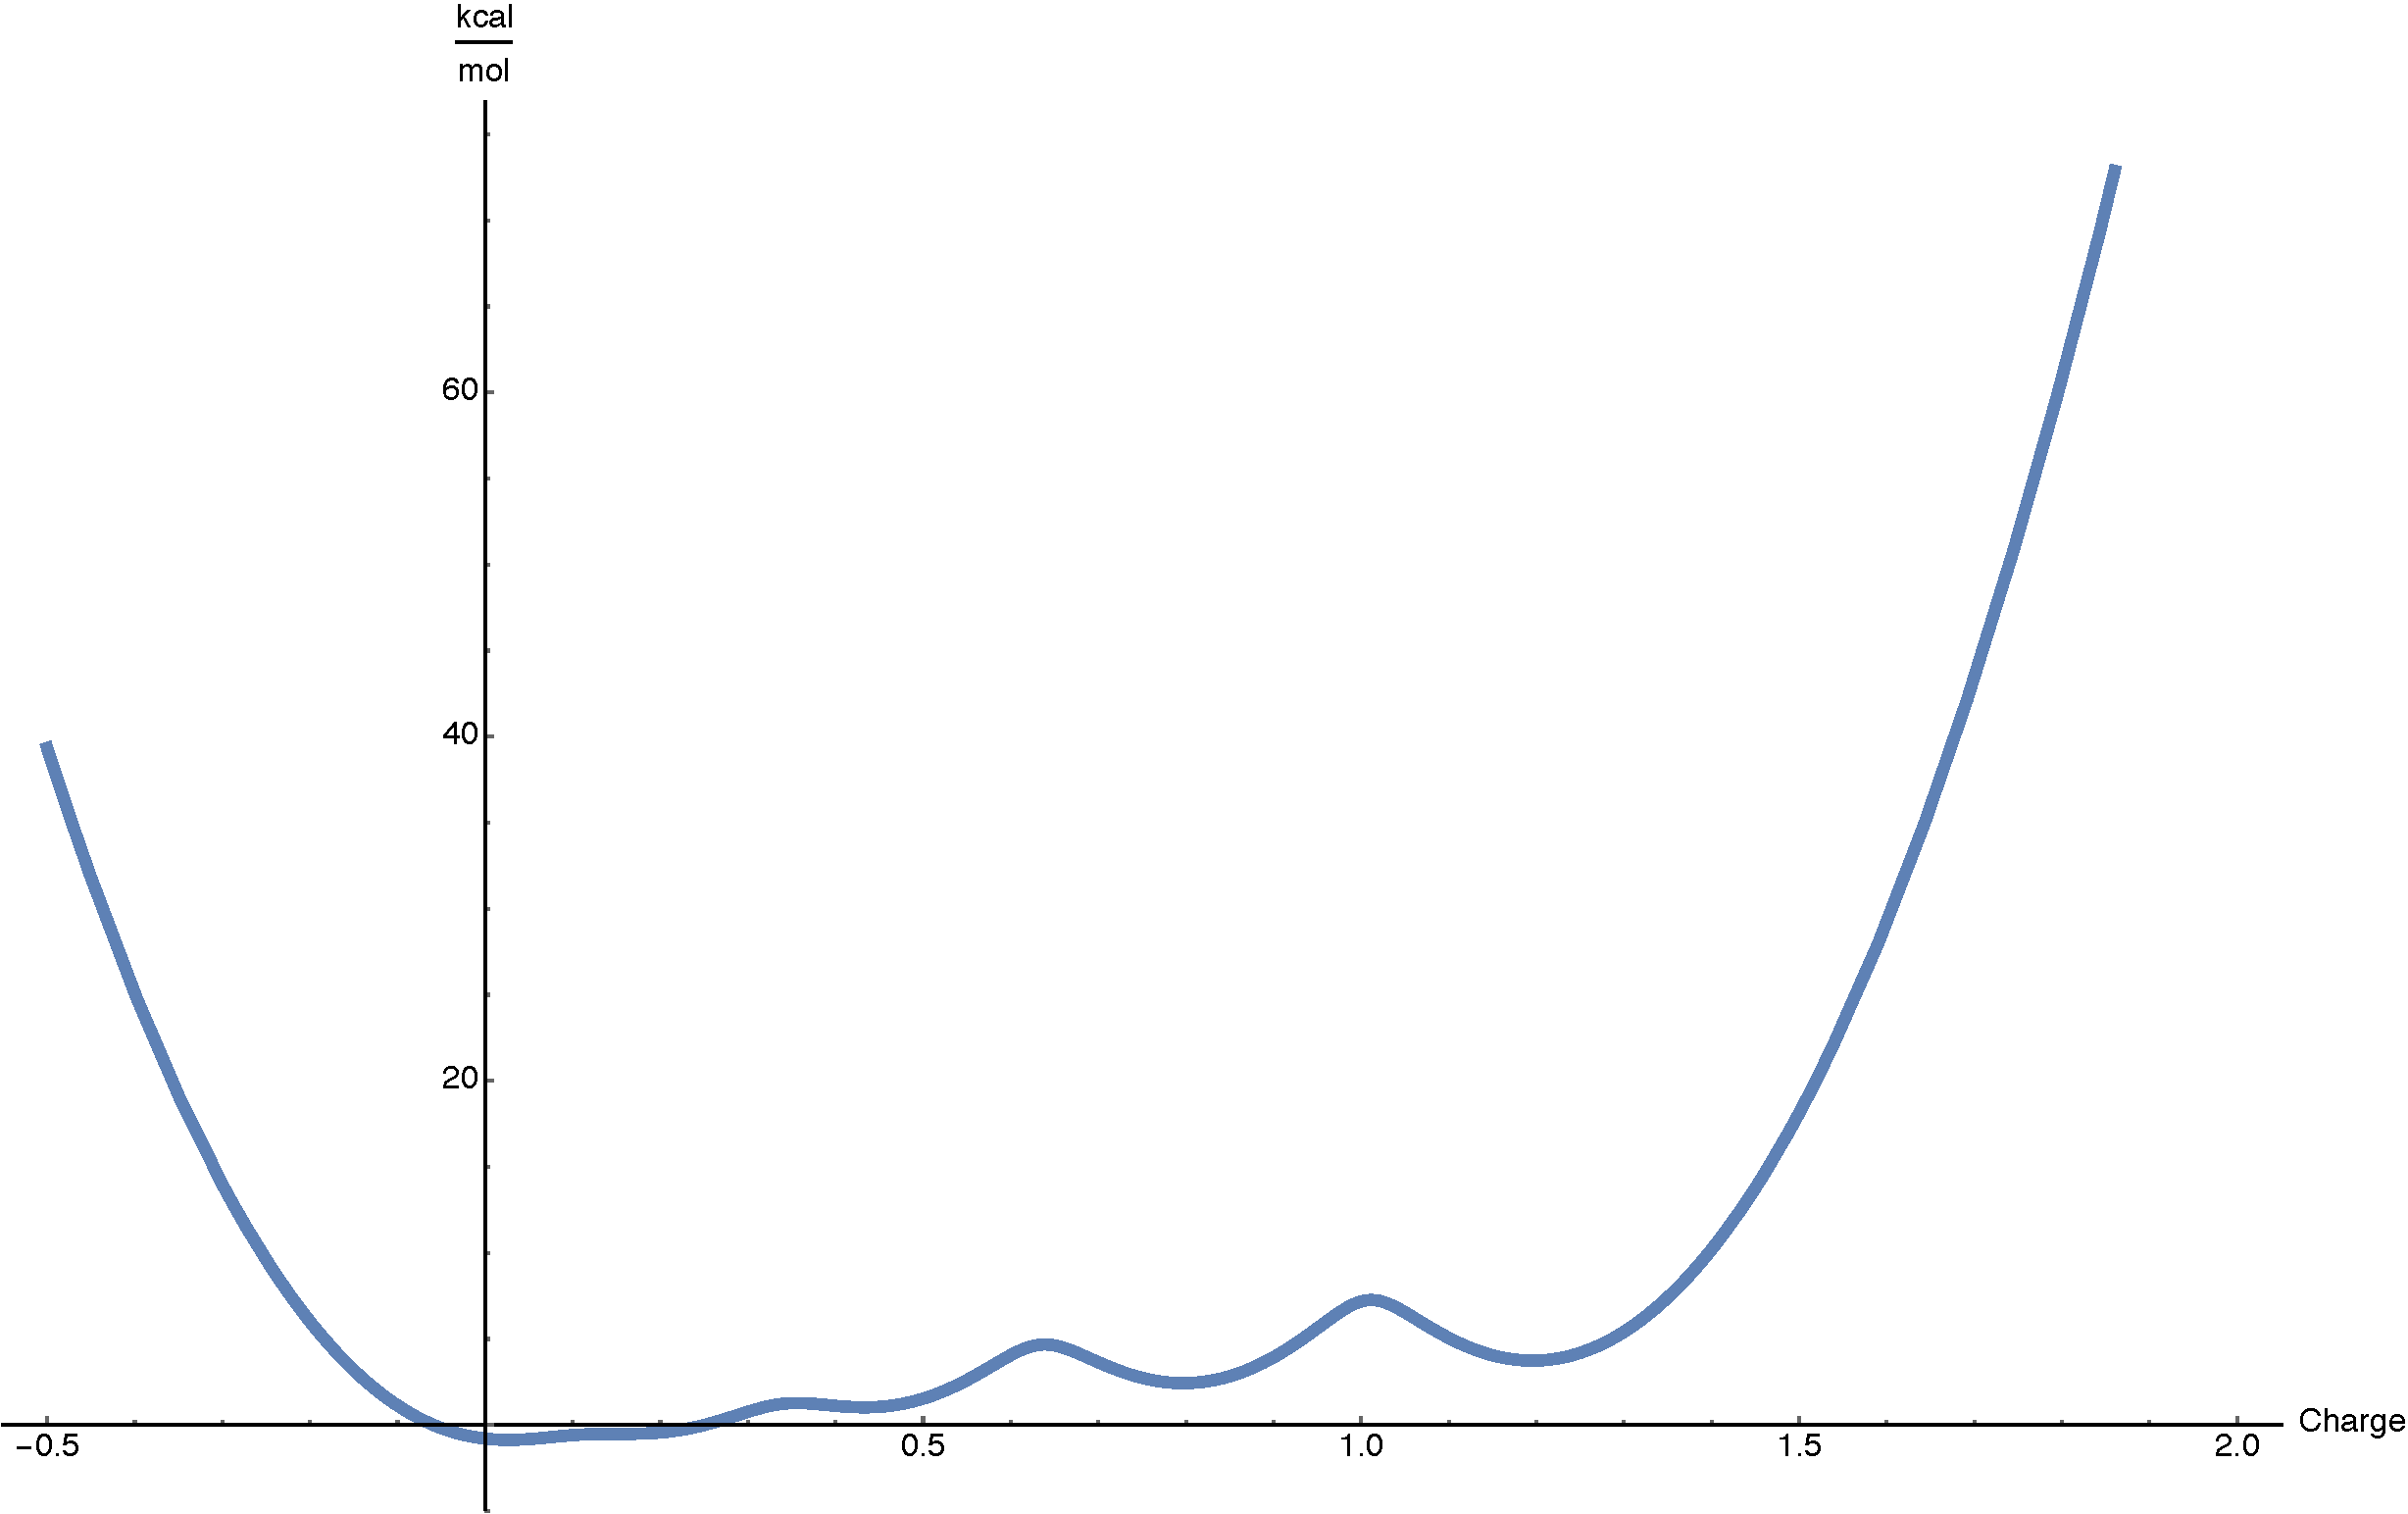
\includegraphics[width=0.75\linewidth]{../figures/chap5/Pt_Charge_Testing.pdf}
  \caption{The self-interaction platinum potential. The parameters to
generate this potential are $[q_0 = 0, q_1 = 0.2, q_2 = 0.45, q_3 = 0.8, q_4 =
1.2, V_0 = 0, V_1 = 1, V_2 = 2, V_3 = 3, V_4 = 4, k = 316, c = 2.5]$.}
\label{fig:PtCharge}
\end{figure}

Using the population analyses to determine valid charge states allows us to
parameterize the $Q_n$ values. The coupling constant $c$ currently has no
experimental justification and is tuned to ensure that a smooth potential is
obtained to minimize issues with integrating the dynamics. The scaling constant
$k$ has been obtained from the atomic/molecular polarizability by using an
ideal two particle system and is explained more fully in the next section.
Finally, the relative energies $V_n$ are currently being arbitrarily set until
we are able to provide theoretical or experimental justifications.

While the potentials in Figure \ref{fig:Ocharge} and \ref{fig:PtCharge} capture
some of the complexity of \ce{Pt\bond{-}O} interactions, for initial fitting
purposes self-energy potentials with 2 and 3 diabatic states are being used for
\ce{O} and \ce{Pt} to minimize the number of needed parameters.

\subsection{Derivation of k}
To estimate a value for $k$, the self-charge force constant parameter in this scheme, we first
created an ideal two-particle system separated by $a_o$, as illustrated in
Figure \ref{fig:kSketch}.  We then arbitrarily shifted one unit of charge
between the otherwise identical atoms. The Hamiltonian of the system is
described below,

\begin{figure}
  \centering
  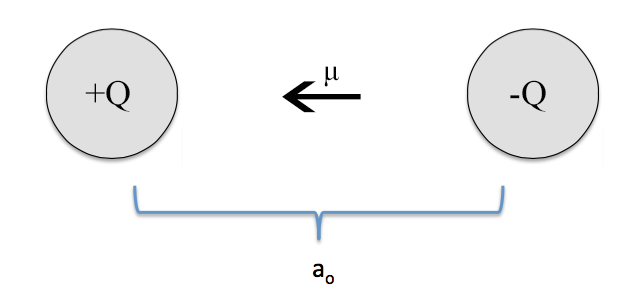
\includegraphics[width=0.75\linewidth]{../figures/chap5/determineK2.png}
  \caption{An ideal system of two particles with a forced charge separation of
$Q$ separated by a distance $a_o$. Constructing the Hamiltonian of this system
allows for a derivation of $k$.}
\label{fig:kSketch}
\end{figure}

\begin{equation*}
H = f_1(+Q) + f_2(-Q) - \frac{Q*Q}{4\pi\varepsilon_o a_o} - \mu\cdot\vec{E}
\end{equation*}

where $f_n(Q)$ describes the kinetic and simplified self-potential of the
atom's charge and is shown below,

\begin{equation*}
f(Q) = \frac{P_Q^2}{2m_Q} + \frac{1}{2}kQ^2
\end{equation*}

The ``charge momentum'' is represented by $P_Q$ and the ``charge mass'' by $m_Q$, while
$k$ is the scaling factor we are deriving. The electrostatic interaction term
and the dipole moment of the system interacting with the local electric field
complete the description of our model. Joining and rewriting the kinetic terms as $T$,
combining like terms, and replacing the dipole moment $\mu$ with $Q\cdot a_o$ leads to the
following,

\begin{equation*}
H = T + Q^2\bigg(k - \frac{1}{4 \pi\varepsilon_o a_o}\bigg) - Q\cdot a_o \cdot \vec{E}
\end{equation*}

The right two terms can be expressed as a shifted harmonic oscillator and can be solved by completing the square,

\begin{equation*}
H = T + a\bigg(Q - \frac{a_oE}{2k - \frac{1}{4\pi\varepsilon_o a_o}}\bigg)^2 + const.
\end{equation*}

with $a = k - \frac{1}{4\pi\varepsilon_o a_o}$.

Recalling that the effective dipole moment is equal to $\mu_{\text{eff}} =
Q_{\text{min}}\cdot a_o$ and $\mu = \alpha\vec{E}$ where $\alpha$ is the atomic
polarizability, we reach the following solution for $k$.

\begin{equation*}
k = \frac{a_o^2}{2\alpha} + \frac{1}{4\pi\varepsilon_o a_o}
\end{equation*}

Using a polarizability for atomic Pt of $\alpha = 6.5$ \AA\textsuperscript{3}
and a nearest neighbor distance of $2.77$ \AA~ for bulk platinum we obtained a
value for $k$ of 316 $\frac{\text{kcal}}{\mathrm{mol\times e}^2}$. Various
polarizabilities and distances can be obtained for oxygen binding to platinum,
all leading to values for $k$ around 280 $\frac{\text{kcal}}{\mathrm{mol\times
e}^2}$.  These values are starting points for the
parameterization rather than as fixed points since the system used to derive
these values is an idealized model and not fully descriptive of the systems we
examined.

\section{Preliminary results}
As full parameterization is still underway, what follows is preliminary results
obtained during attempted parameterizations of forcefields for platinum oxide
systems. Specifically, one of the systems we model is composed of a negatively
charged oxygen atom approaching a (111) platinum surface. 
Since the mm-FlucQ method assume that a species electrons are collapsed
as point charges on the atomic sites, for the time being, anisotropy is not being considered. 

To visualize the charge density in these systems we begin by defining a uniform
grid of points (spacing approximately 1 \AA) spread throughout the simulation
box. The electron density as contributed by nearby atomic sites, assuming a
Gaussian distribution, is summed at each grid point and then assembled to use in
a volume rendering program. With regards to the electron
density, we treat density at a site $i$ with a three dimensional Gaussian
function as shown below,

\begin{equation*}
\rho(\vec{\mathbf{r}}) = \sum_i q_{i} \frac{1}{(2\pi)^{3/2}}e^{\frac{-(\vec{\mathbf{r}}-\vec{\mathbf{r}}_i)^2}{2}}
\end{equation*}

where our isotropic requirement leads to $\sigma_x = \sigma_y = \sigma_z = 1$,
$q_i$ is the charge of atom $i$ and $\Delta r$ is the distance from the point
where the density is being measured to the position of the atomic site
$\vec{\mathbf{r}}_i$. 

As seen in Figure \ref{fig:chargeVol}, which depicts an \ce{O-} ion approaching
a charge responsive \ce{Pt} surface, most of the metal atoms experience minimal
disruption away from the neutral ground state, whereas the metal directly
beneath the \ce{O-} ion gains a significant amount of positive charge. The
units of charge density are 0.001 $e^-$/\AA\textsuperscript{3} as calculated from the
above Gaussian. Figure \ref{fig:chargeHistogram} provides another view of this
system by looking at the charge population of the \ce{Pt} at various times over
the simulation length.

\begin{landscape}
\begin{figure}
  \centering
  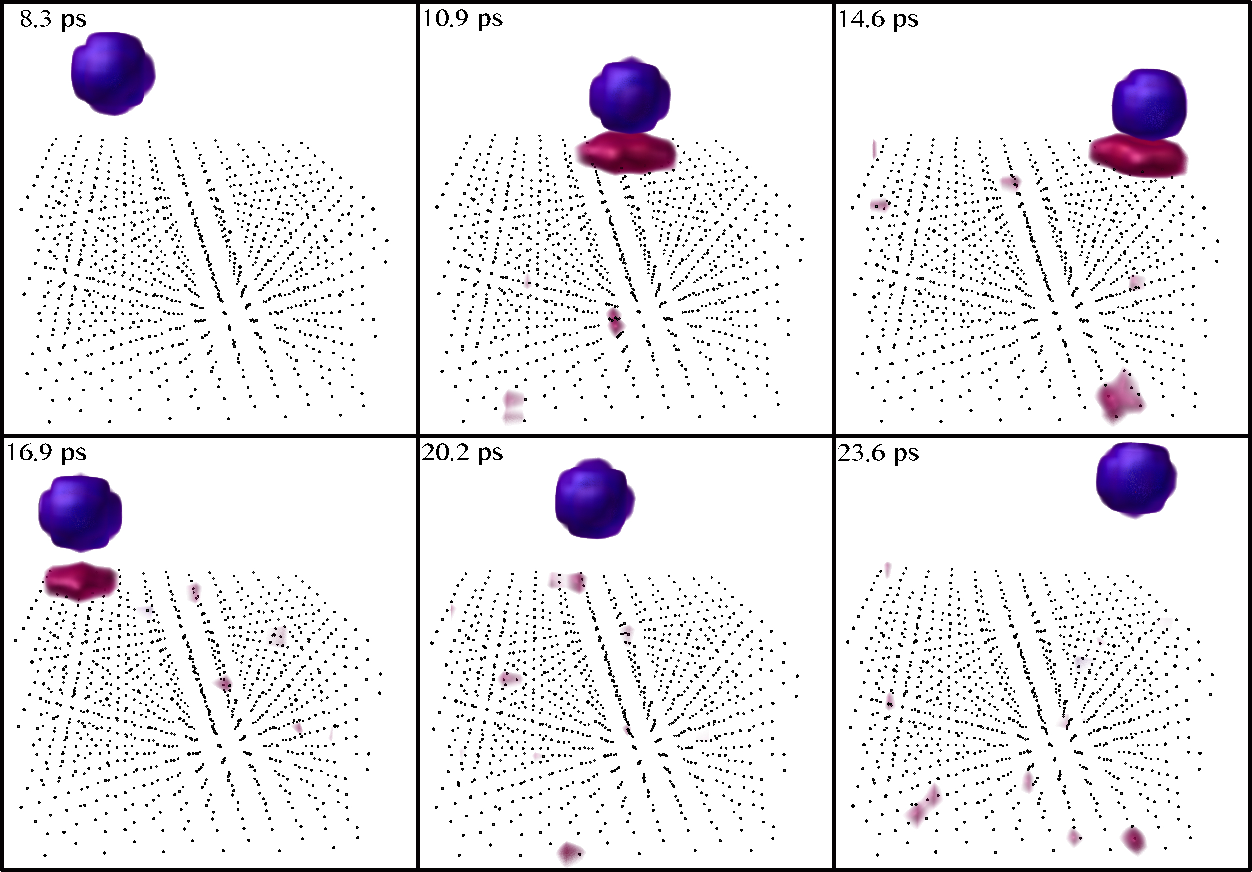
\includegraphics[width=0.7\linewidth]{../figures/chap5/PtOChargeVolume.pdf}
  \caption{As the oxide ion (\ce{O-}) approaches the surface, the \ce{Pt} directly beneath
the \ce{O-} loses electron density leading to a favorable interaction between
the \ce{Pt} and \ce{O-}. Units are in $0.001\ e^-$/\AA\textsuperscript{3},
however only the extremes of charge density are rendered.}
\label{fig:chargeVol}
\end{figure}
\end{landscape}

\begin{figure}
  \centering
  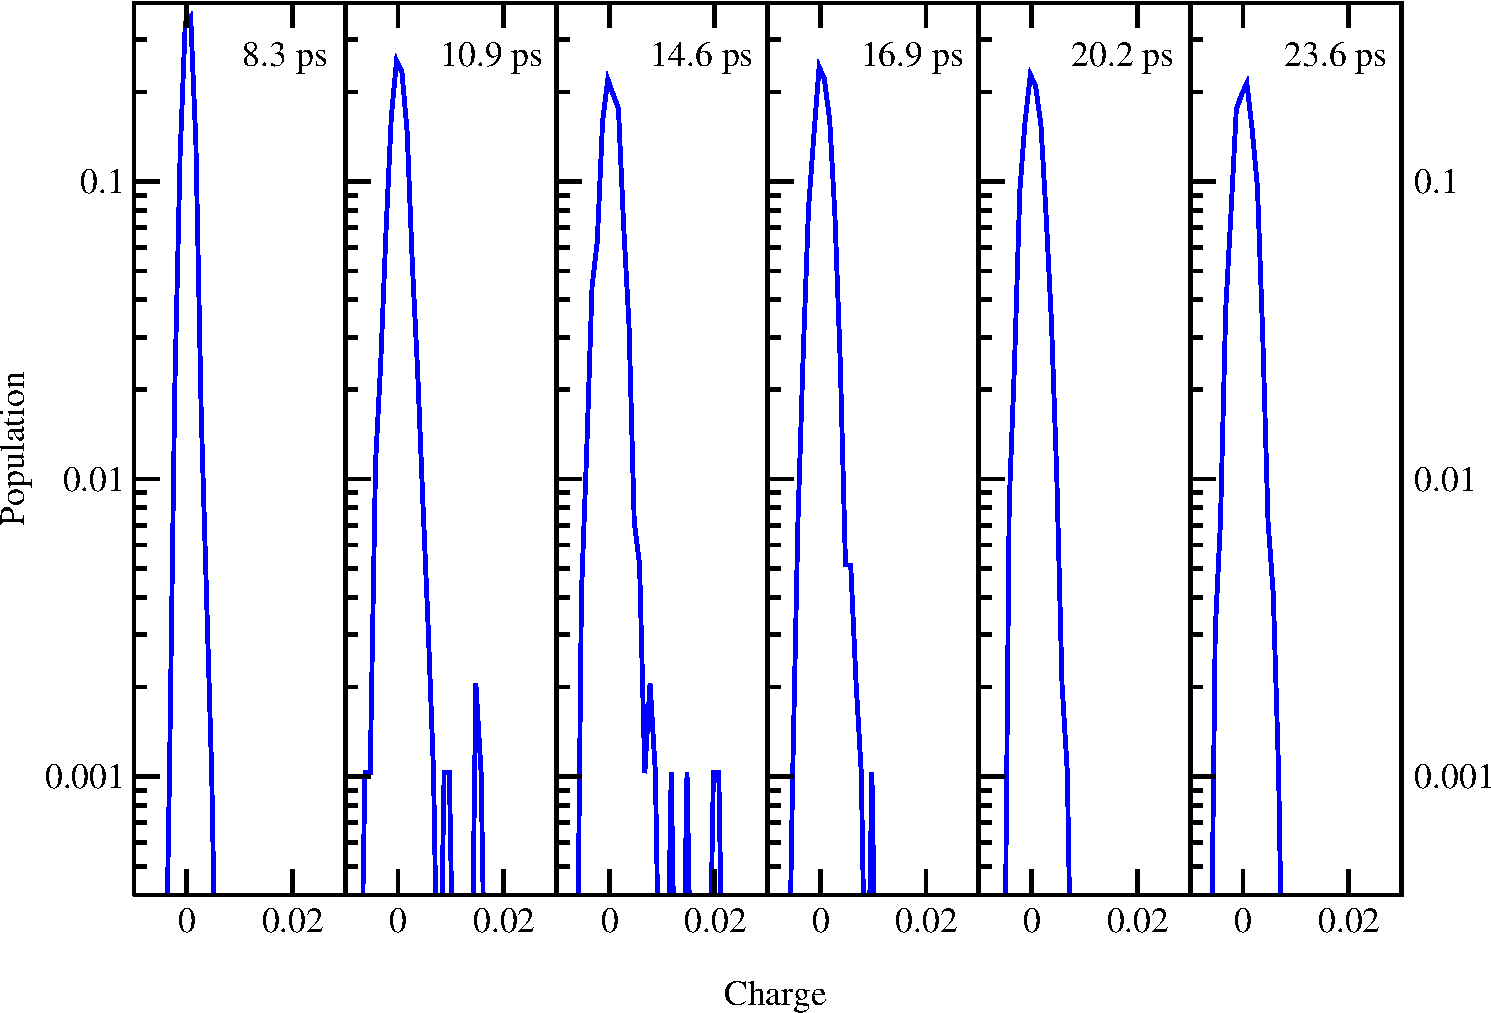
\includegraphics[width=0.9\linewidth]{../figures/chap5/frameChargeDistribution.pdf}
  \caption{Charge distributions in \ce{Pt} corresponding to the snapshots
depicted in Figure \ref{fig:chargeVol}. As the bulk of the metal is unaffected, a
logarithmic $y$-axis is utilized to highlight the atoms that deviate from 0
charge. As \ce{O-} approaches the surface, small peaks corresponding to surface
\ce{Pt} atoms with a positive charge appear. As the charge is smeared
out over a handful of \ce{Pt} atoms, each one tends to approach 0.02 $e^-$.}
\label{fig:chargeHistogram}
\end{figure}

\section{Future directions}
While this method has succeeded in capturing the movement and accumulation of
charge in a metal surface in response to an incoming ion, accurate
parameterization of the numerous parameters is still on-going. Additionally,
the build-up of charge at the surface rather than at some depth $d$, appears to
be in violation of the method of images. Further work is thus needed to
properly incorporate the electrical potential being constant at the surface of
a conductor.  This work is on-going and when completed opens up a large realm
of possible directions of studies, specifically, oxide formation on platinum is
of immense interest. Additional interactions with metal surfaces will also be
explored with this technique and will include small molecules, {\em i.e.}
\ce{CO}, \ce{H2O}, \ce{NO}, etc., metal ions, and small biological analogs like
that amino acids and short peptide chains.





\chapter{CONCLUSIONS}

%

In this dissertation I have presented new forcefields for \ce{CO} interacting
with \ce{Pt} as well as illustrating the mechanisms of surface reconstructions
as it relates to step-edge doubling and island formation. I have further examined the effects of displayed step-type on the 


\subsection{Alternative Systems of Interest}
This dissertation has focused on the well-studied \ce{Pt}-\ce{CO} interactions
and only branched out by examining \ce{CO} interactions with \ce{Au} and
\ce{Pd}.  There are numerous adsorbate-metal systems that have been identified
as also undergoing various types of reconstruction including \ce{CO} and
\ce{O2} over \ce{Rh\bond{-}Pt} core-shell nanoparticles,\citep{Tao:2008aa},
\ce{CO} over \ce{Cu} (111),\citep{Eren:2016qt} \ce{CO} and \ce{O2} over a (553)
\ce{Rh} surface,\citep{Zhang:2015zr}, \ce{CO} over a \ce{Pd/Au} bimetallic
surface,\citep{Kim:2013mi} and many more. The majority of these are experimental
studies which are often unable to directly identify the mechanism of the
reconstruction making them of potential interest to model.

Despite \ce{Pt\bond{-}Pd} bimetallic catalysts being of considerable interest,
both components are relatively expensive and significant effort is being
expended to tailor \ce{Pt\bond{-}M} surfaces and nanoparticles.
\ce{Pt\bond{-}Ni} is of immense interest because of its increased activity for
the oxygen reduction reaction and would be of much interest to
model.\citep{Tuaev:2013fk, Stamenkovic:2007kk,Sneed:2014fj}

As the Multiple Minima Fluctuating Charge method is continually refined, many
avenues for exploration are opened, especially those involving charged
adsorbates on metal surfaces. Many systems and processes of interest, including
\ce{H2O} on \ce{Pt},\citep{Xu:0dz} metallic-oxide
formation,\citep{Streitz:1994mw, Fantauzzi:2014pb, Lloyd:2016jt}, and various
biological molecules on metal surfaces,\citep{Padmos:0qf, Mete:2015rc} which
have been studied at differing levels of theory would be benefitted by more
fully treating the electrostatic interactions present in the system. 



\appendix

 % If you have appendices, add them here.
 % Begin each one with \chapter{TITLE} as before- the \appendix command takes
 % care of renaming chapter headings and creates a new page in the Table of
 % Contents for them.
 % \include{appendix-one}


\chapter{CO ADSORPTION PATTERNING AND EXPANDED DOMAIN FIGURES}


The new \ce{Pd}-\ce{CO} potential energy function discussed in the
main text recovers the experimental $c(4 \times 2)$ surface structure
at high coverages.  In figure \ref{fig:C4x2}, we show that relatively
large domains of $c(4 \times 2)$ ordered \ce{CO} form on the surface.
The surface was prepared as a perfect \ce{Pd}(111) at 500~K, and was
dosed with a 0.5 ML coverage of gas phase \ce{CO}.  The system was
then cooled from 500~K to 130~K over 2~ns.  The domains and incomplete
ordering are a result of the rapid cooling.

\begin{figure}
  \includegraphics[width=\linewidth]{../figures/appA/C4x2_best.pdf}
  \caption{0.50 ML of \ce{CO} on a \ce{Pd}(111) surface adopts domains
    (outlined in cyan boundaries) of the $c(4 \times 2)$
    configuration. The surface started at 500~K and was cooled to
    130~K over 2~ns.  At this relatively high cooling rate, multiple
    domains with different orientations of the $c(4 \times 2)$ pattern
    are displayed.}
\label{fig:C4x2}
\end{figure}

\newpage

The newly-fit \ce{Pt}-\ce{CO} potential energy function discussed in
the main text recovers the experimental
$(\sqrt{3} \times \sqrt{3}) R~30^{\circ}$ surface structure at a 1/3
ML coverage.  In figure \ref{fig:Root3}, we show that small domains of
$(\sqrt{3} \times \sqrt{3}) R~30^{\circ}$ ordered \ce{CO} form on the
surface.  The surface was prepared as a perfect \ce{Pt}(111) at 500~K,
and was dosed with a 0.33 ML coverage of gas phase \ce{CO}.  The
system was then cooled from 500~K to 130~K over 10~ns.  The small
domains and incomplete ordering are a result of the relatively rapid
cooling.

\begin{figure}
  \includegraphics[width=\linewidth]{../figures/appA/Pt_33_root3.pdf}
  \caption{0.33 ML of \ce{CO} on a \ce{Pt}(111) surface adopts domains
    (outlined in cyan boundaries) of the
    $(\sqrt{3} \times \sqrt{3}) R~30^{\circ}$ configuration. The
    surface started at 500~K and was cooled to 130~K over 10~ns.  At
    this cooling rate, small domains with different orientations of
    the $(\sqrt{3} \times \sqrt{3}) R~30^{\circ}$ pattern are
    displayed.}
\label{fig:Root3}
\end{figure}

\newpage

An expanded version of figure 3 in the main text which contains data
for all five \ce{CO} coverage levels.

\begin{figure}
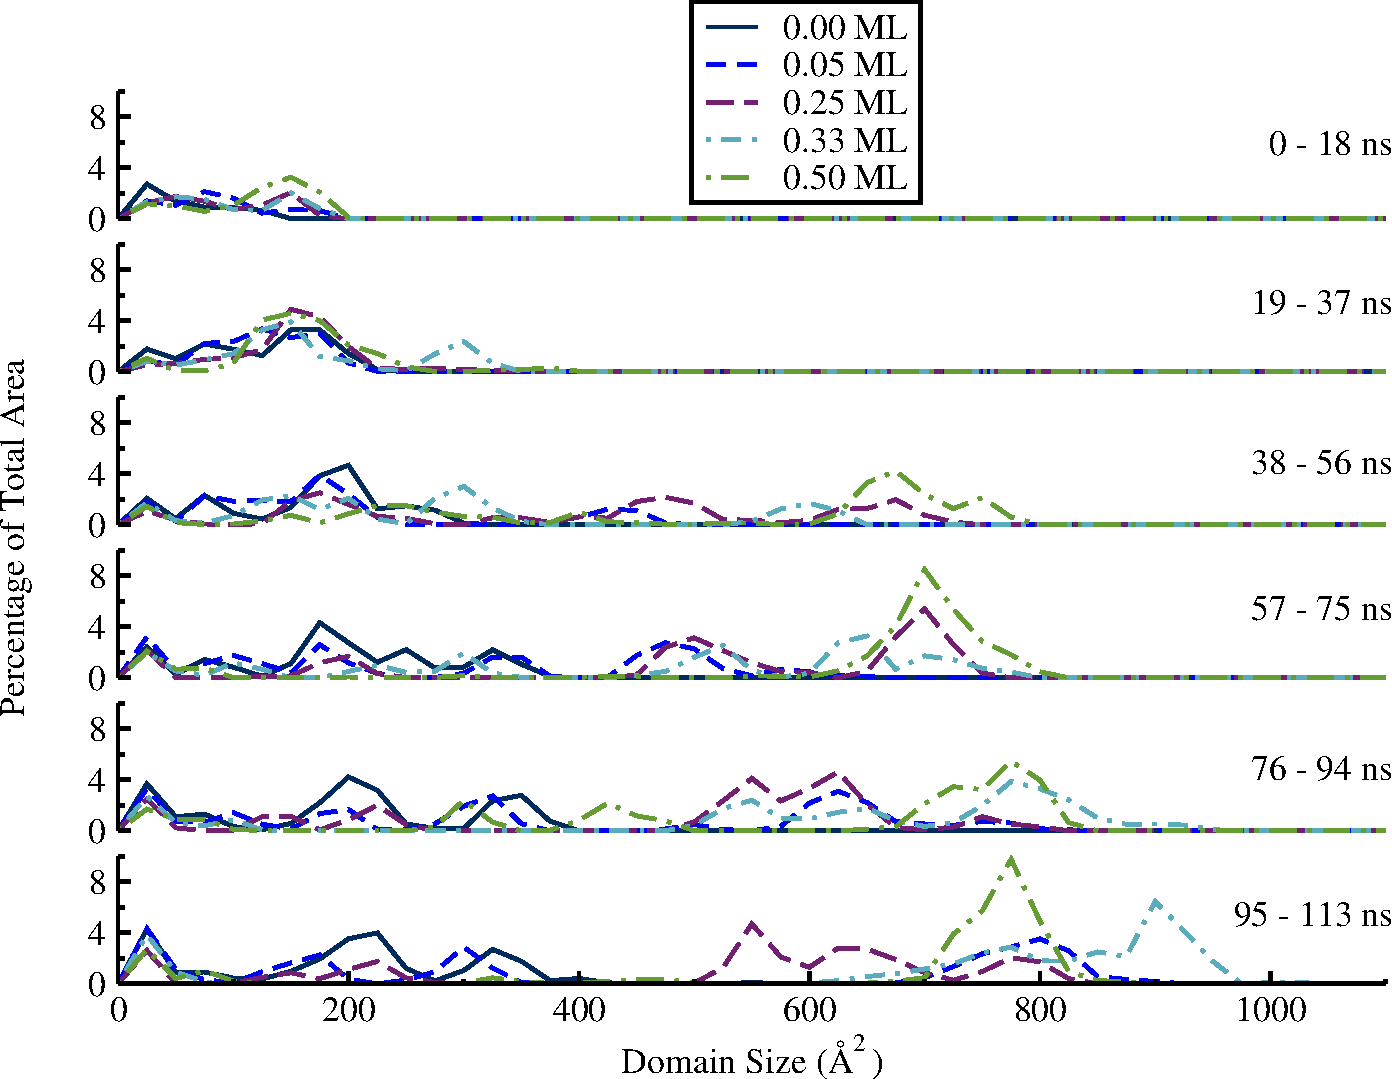
\includegraphics[width=\linewidth]{../figures/appA/domainSize_Pd_SI.pdf}
\caption{Distributions of \ce{Pd} domain sizes at all simulated
\ce{CO} coverages at different times after exposure to \ce{CO}.}
\label{fig:Pd_SI}
\end{figure}

\newpage

An expanded version of figure 4 in the main text which contains data
for all five \ce{CO} coverage levels.

\begin{figure}
  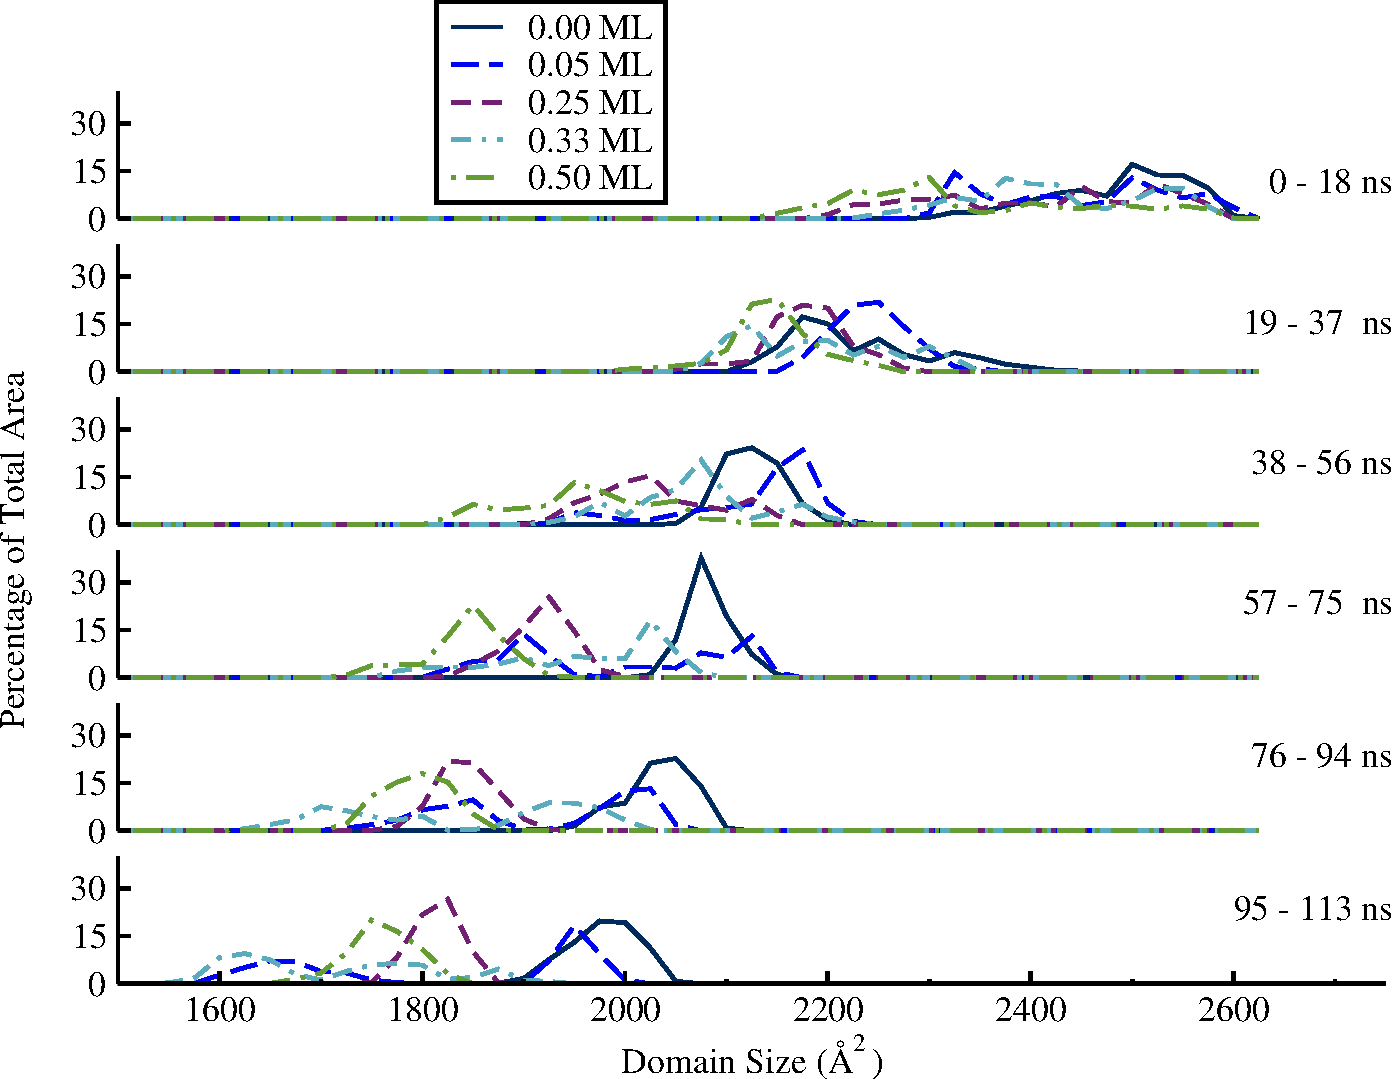
\includegraphics[width=\linewidth]{../figures/appA/domainSizes_Pt_SI_zoomed.pdf}
  \caption{Distribution of large \ce{Pt} domain sizes at all simulated
    \ce{CO} coverages at different times after exposure to \ce{CO}.}
\label{fig:Pt_SI_big}
\end{figure}

\newpage

Figure \ref{fig:Pt_SI_small} contains data on the \ce{Pt} domains that
were $<$ 100 \AA\textsuperscript{2} in area.  Typical domains with
larger surface areas typically comprise 15-20\% of the total area,
while these smaller domains never reach 1\% of the total. These
domains correspond to 1-to-2 atom clusters of \ce{Pt} that exist
surrounded by \ce{Pd}. This situation can arise either from \ce{Pt}
adatom movement over the \ce{Pd} surface, or \ce{Pt}-\ce{Pd}
inversion.

\begin{figure}
  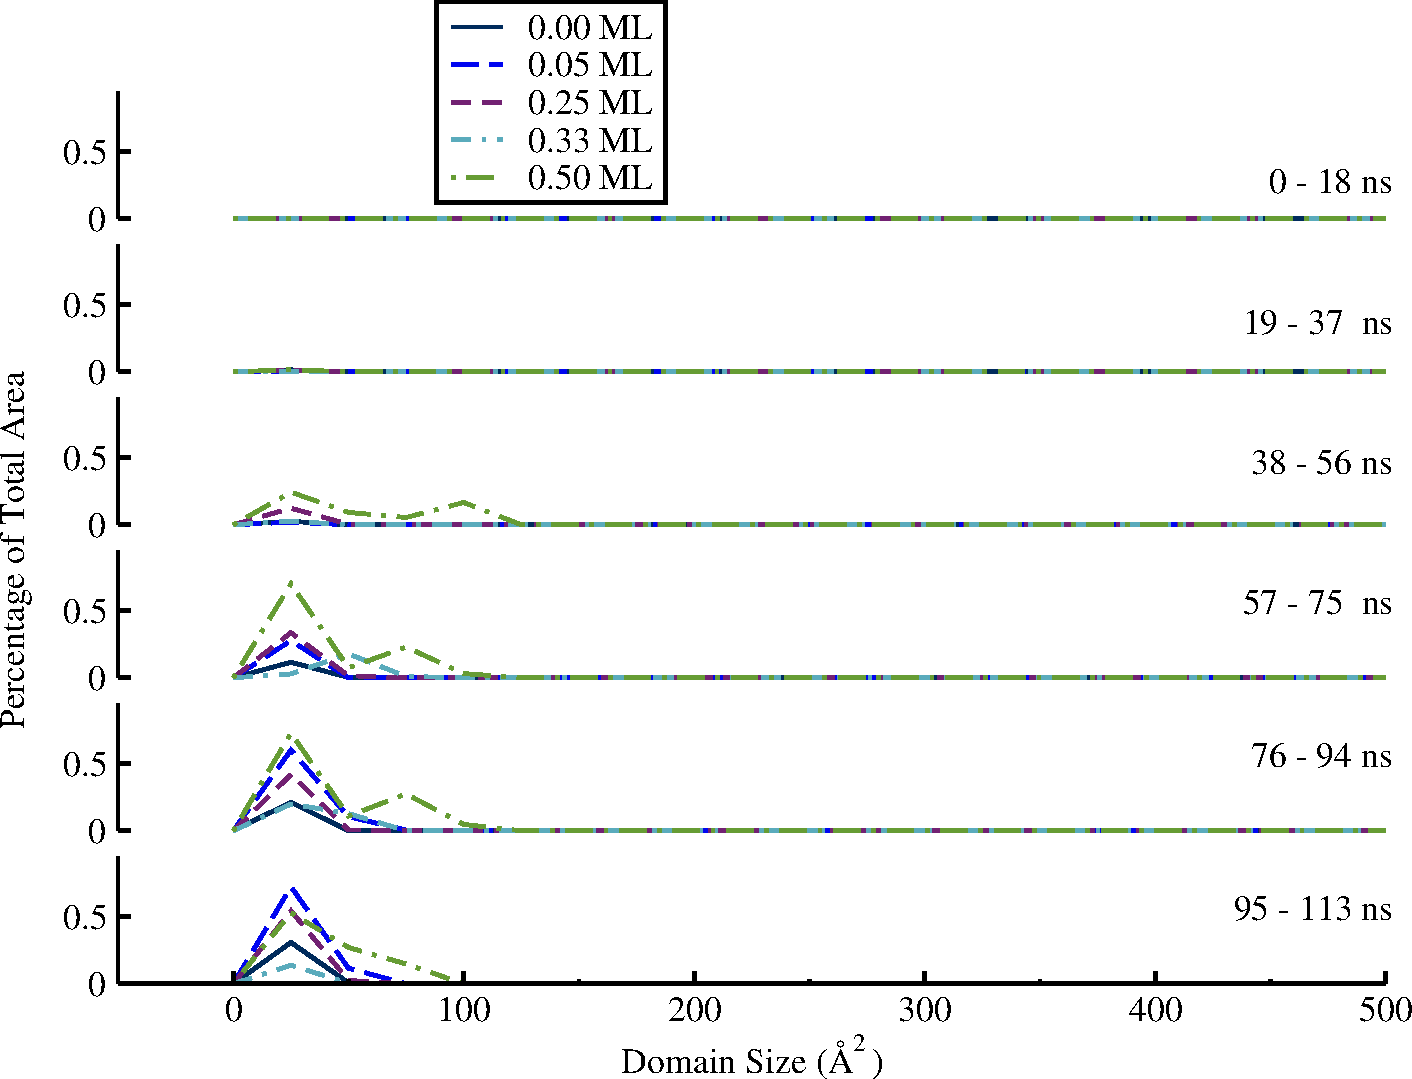
\includegraphics[width=\linewidth]{../figures/appA/domainSizes_Pt_SI_smallFocus.pdf}
  \caption{Distribution of small \ce{Pt} domain sizes at different
    \ce{CO} coverages and at different times after exposure to
    \ce{CO}. Note that the $y$-axis is significantly smaller than in
    figure 4 in the main text.}
\label{fig:Pt_SI_small}
\end{figure}


\newpage

In the surface alloys, the reconstruction involves mostly \ce{Pt} atom
motion, leaving the underlying \ce{Pd}(557) substrate mostly intact.
This is easily seen when the \ce{Pt} atoms in the left image below are
hidden.  The small amount of step-wandering and step-breaking of the
underlying \ce{Pd} highlighted on the right side of fig. \ref{fig:557}
shows the strong tendency of \ce{Pd} to maintain the (557) steps.
Additionally, the main deviations of the \ce{Pd} substrate observed
here appear to be tied to the locations of islands in the \ce{Pt} top
layer.

\begin{figure}
  \includegraphics[width=\linewidth]{../figures/appA/557.pdf}
  \caption{Snapshots of the \ce{Pt}/\ce{Pd} 0.33 ML system after
    $\sim$110~ns (\ce{CO} hidden). The right panel highlights the
    stability of the underlying (557) \ce{Pd} substrate after hiding
    the surface \ce{Pt} atoms. \ce{Pt} atoms are shown in gray and
    \ce{Pd} atoms are shown in pink.}
\label{fig:557}
\end{figure}

\newpage

An expanded version of figure 5 in the main text which contains data
for all five \ce{CO} coverage levels.  The ordering of the coverages
is fairly well maintained, although the 0.25 and 0.33 ML curves cross
at a number of points.

\begin{figure}
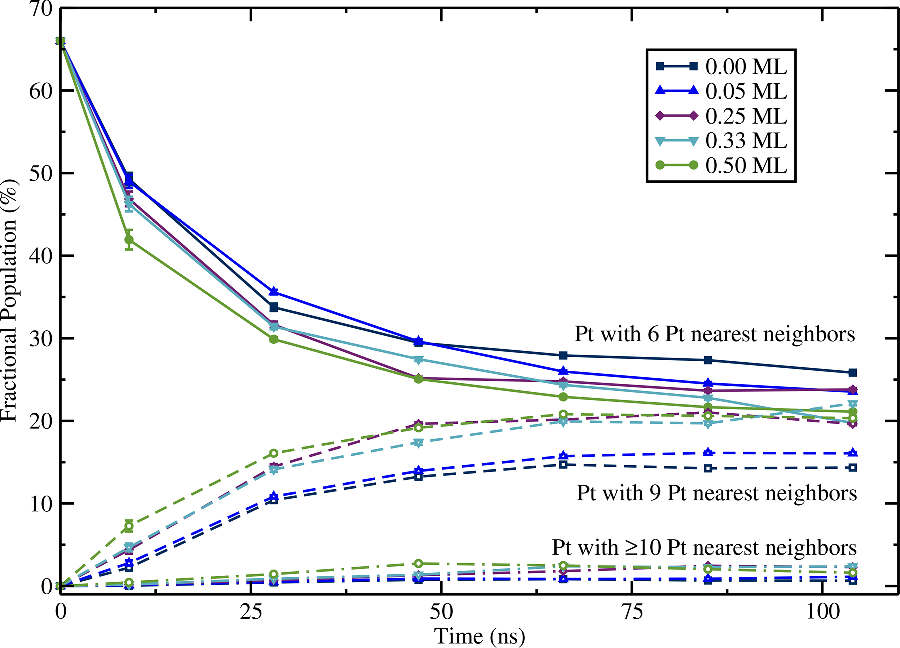
\includegraphics[width=\linewidth]{../figures/appA/nearestNeighbor_full_withmorenn_photoshopped.pdf}
\caption{Population of \ce{Pt} atoms with either 6 (solid), 9
  (dashed), or $\ge$ 10 (dot-dashed) \ce{Pt} nearest neighbors
  averaged over 18~ns blocks of time.  At $t = 0$, the majority
  (2/3) of \ce{Pt} is located in the (111) plateaus where
  the number of \ce{Pt} nearest neighbors is 6. The remaining \ce{Pt}
  is located at step edges, with a neighbor \ce{Pt} count of 5.}
\label{fig:nn_full} 
\end{figure}








\chapter{ADDITIONAL GENERALIZED COORDINATE NUMBER FIGURES AND SYSTEM IMAGES FOR PLATINUM (321), (112), (765) \& (557)}
\label{app:SI2}


Shown in this appendix are supporting figures for Chapter \ref{chap:facet}.
Additional GCN plots as well as system figures are displayed below.
\newpage



The step-wandering all of the surfaces exhibit during the simulation can hinder
an easy interpretation of the generalized coordinate figures. Figure
\ref{fig:557GCN} provides an additional ideal surface to complement the (321)
figure shown in chapter \ref{chap:facet}. The roughness of the (557) surface is
less than that of the (321) surface which is shown by the fewer number of GCN
peaks. 

\begin{figure}
\centering
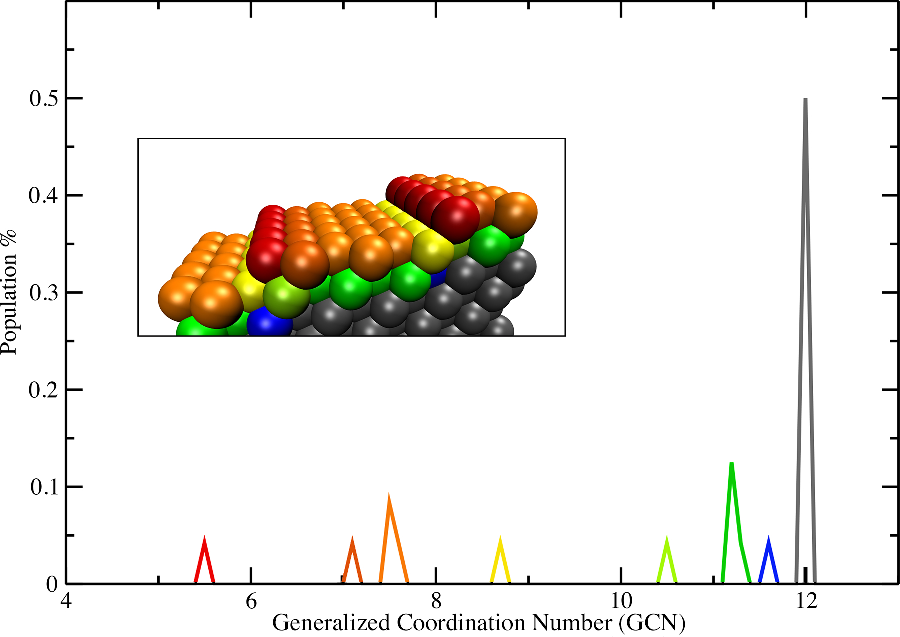
\includegraphics[width=0.9\linewidth]{../figures/appB/557_ideal_gcn.pdf}
\caption{A graph of the generalized coordinate number of an ideal Pt (557)
system colored to match the inset figure. Other than the bulk (GCN=12), the
(557) surface displays three primarily different surface sites, the edge atoms
(red, GCN=5.5), the plateaus (orange, GCN=7.2,7.5) and the slightly eclipsed
atoms beneath the step (yellow, GCN=8.7). Subsurface atoms have a larger GCN
than the surface atoms, but are still less than the bulk GCN of 12.}
\label{fig:557GCN}
\end{figure}
\newpage


As the \ce{Pt} (557) did not undergo step doubling in these simulations, the
generalized coordinate numbers describing the system were not expected to
largely change, as seen in Figure \ref{fig:557lsGCN}.

\begin{figure}
\centering
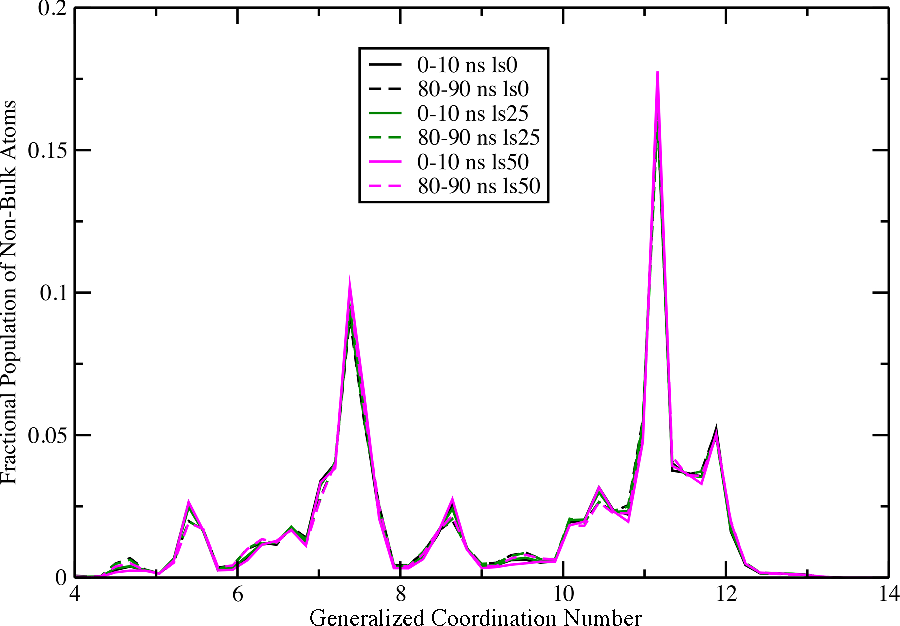
\includegraphics[width=0.9\linewidth]{../figures/appB/557ls_GCNF.pdf}
\caption{Plots of the average GCN for the non-bulk atoms of the \ce{Pt} (557)
LS systems. Solid lines represent the averaged GCN during the first 10
nanoseconds of simulation time, while the dotted lines correspond to a time
near the end of the simulations. Black, green and magenta lines depict the 0,
0.25, and 0.5 ML systems respectively. Except for a slight decrease at 5.5 and
10.5, minimal changes were observed.}
\label{fig:557lsGCN}
\end{figure}
\newpage


The slight increase in the peak at GCN=7.5 suggests that this measurement is
sensitive to minor surface reconstructions, like the step-edge doubling and
disappearance highlighted in Figure \ref{fig:765Edge}. Beyond that
reconstruction on the MS 0.5 ML system, very little besides step-wandering was
observed on the (765) surfaces.

\begin{figure}
\centering
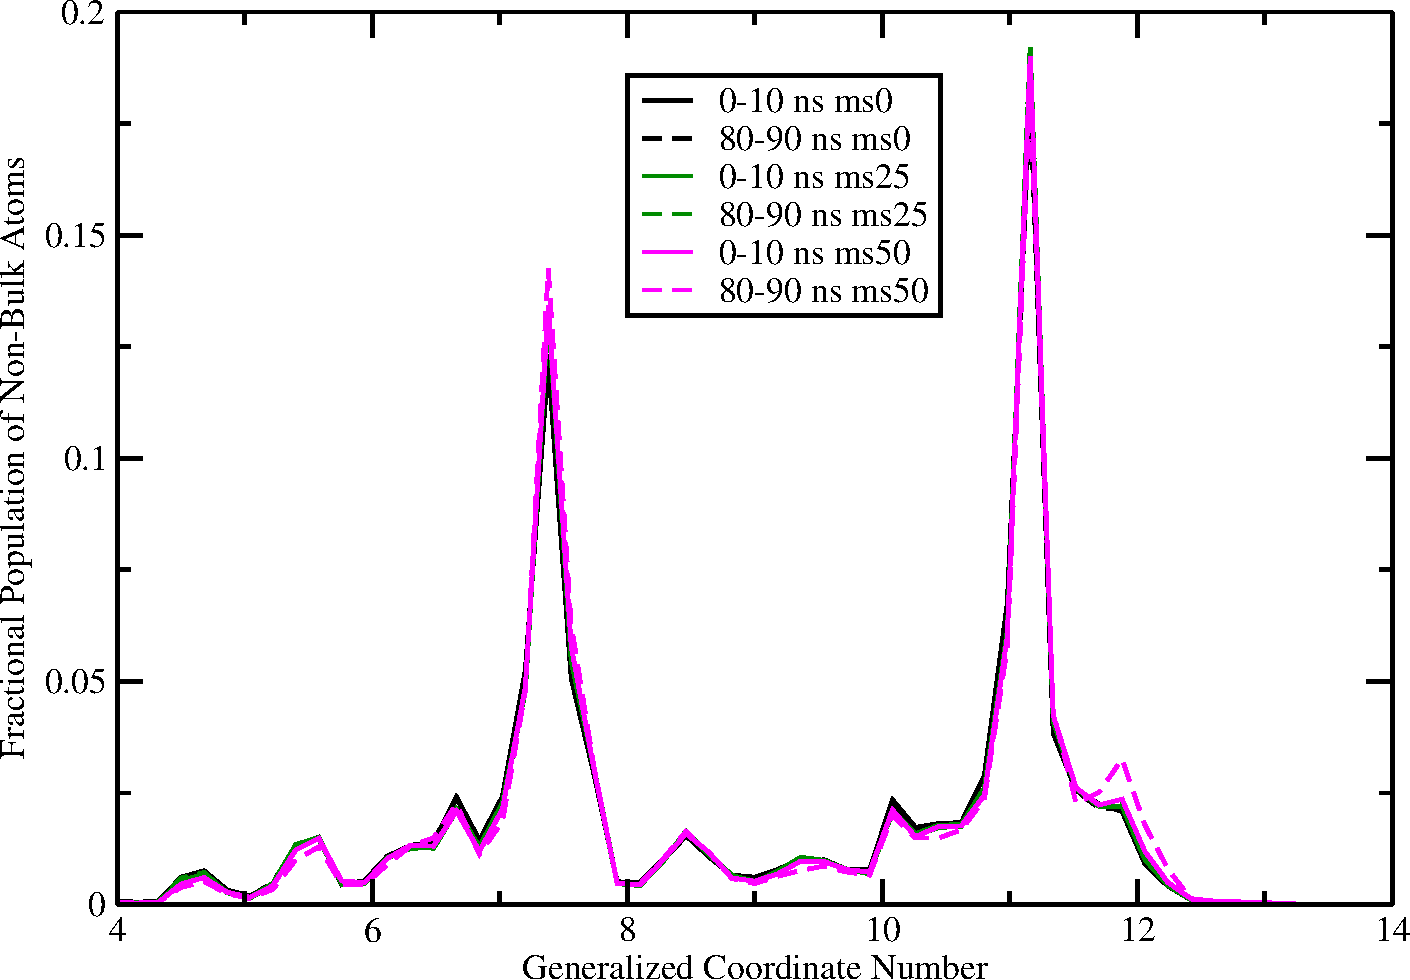
\includegraphics[width=0.9\linewidth]{../figures/appB/765ms_GCNF.pdf}
\caption{Plots of the average GCN for the non-bulk atoms of the \ce{Pt} (765)
MS systems. The slight increases seen at 7.5 and 11.8 capture the
pseudo-doubling process explored in Figure \ref{fig:765Edge}.}
\label{fig:765msGCN}
\end{figure}
\newpage

The increase in the peak at GCN=6.8 for the 0.0 and 0.5 ML LS systems appears
to be capturing the loss of the clean (765) surface observed on both of these
systems. The 0.25 ML LS system in contrast only underwent some step-edge
wandering, but generally maintained its displayed edges.

\begin{figure}
\centering
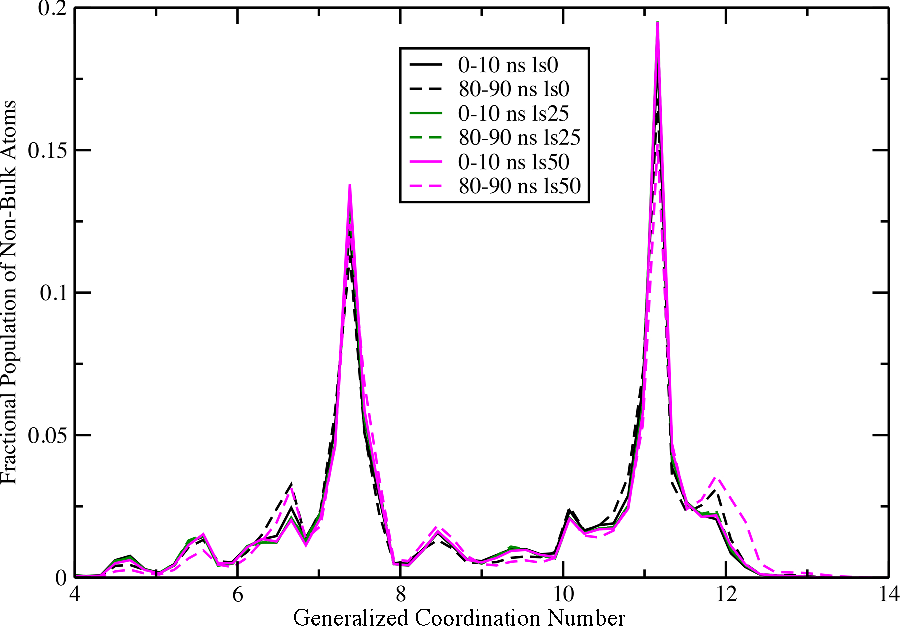
\includegraphics[width=0.9\linewidth]{../figures/appB/765ls_GCNF.pdf}
\caption{Plots of the average GCN for the non-bulk atoms of the \ce{Pt} (765)
LS systems. The slight increases seen at 6.8 and 11.8 for the 0.0 and 0.5 ML
systems appears to capture the disruption seen on these surfaces.}
\label{fig:765lsGCN}
\end{figure}
\newpage

The (112) systems explored in this study suffer from a slight instability at
the temperatures simulated that led to a number of the step-edges sinking
partially into the surface. As highlighted in Figure \ref{fig:112sunken}, a few
of the edges maintained their (100) step facet and were often seen to be a
source for adatom formation. The steps that sunk into the surface conversely,
rarely ejected adatoms and for the majority of the simulation time underwent
minimal movement on the surface.

\begin{figure}
\centering
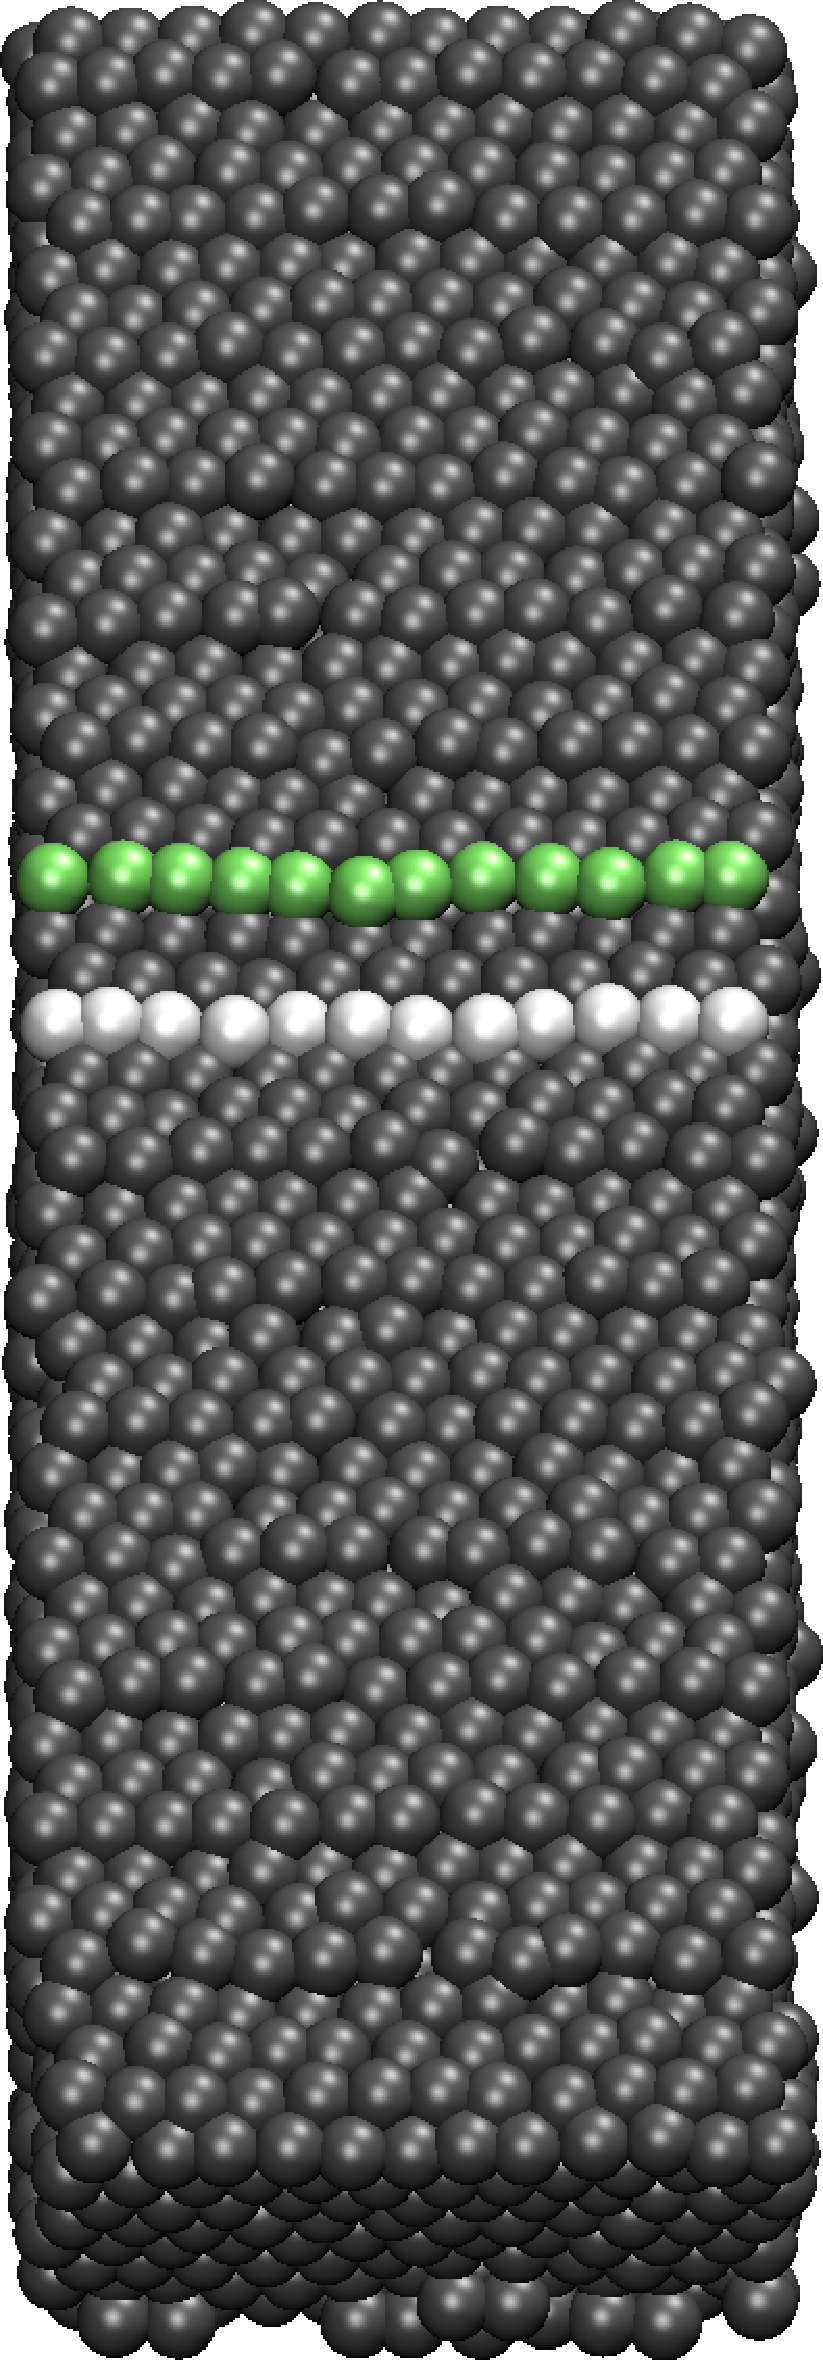
\includegraphics[width=0.3\linewidth]{../figures/appB/112_sunken.pdf}
\caption{The (112) systems, because of their large surface energy underwent a
minor refaceting that resulted in many of the (100) steps sinking slightly into
the surface (white) and displaying a (111) sunken edge. A few step edges (lime)
retained their (100) step edge morphology and were often the source for adatom
formation.}
\label{fig:112sunken}
\end{figure}
\newpage


%\begin{figure}
%\includegraphics[width=0.8\linewidth]{../figures/appB/321MiniDiamonds}
%\caption{The energy required to translocate a kinked atom along the step edge
%is minimal, and on the (321) surfaces this leads to the formation of numerous
%small (111) diamonds on the surface. Systems are shown at (a) the beginning and
%(b)-(c) the end (100 ns) of the simulation for the (112) LS 0.25 ML system.
%While some step-edge doubling is observed, a significant portion of the surface
%has been replaced with these small diamond domains.}
%\label{fig:321Diamonds}
%\end{figure}
%\newpage

The rough edges and large plateaus of the (765) systems were expected to help
distinguish which surface attributes were most important in encouraging or
hindering surface reconstruction. Unexpectedly, no obvious step-doubling
occurred on these surfaces despite a significant amount of step-wandering
taking place. One event that occurred on the 0.5 ML MS system is displayed in
Figure \ref{fig:765Edge}. What is originally two separate roughened steps, over
the course of the simulation becomes a single step located at an intermediate
distance between the original steps. It appears as if a portion of each step
sinks into the surface leaving the two other sections to meet up to form a
single step edge.

\begin{landscape}
\begin{figure}
\centering
\includegraphics[width=0.9\linewidth]{../figures/appB/765MissingEdge.pdf}
\caption{The (765) MS 0.5 ML system (a) 0 ns, (b) 33.4 ns, (c) 50.2 ns, (d)
75.1 ns, (e)100 ns after exposure to CO underwent an intriguing reconstruction.
The identified step-edges in (a), approach each other while also each starting
to sink somewhat into the surface. The result in a step-edge that is between
the starting points of either parent, but still of only one atomic height.}
\label{fig:765Edge}
\end{figure}
\end{landscape}
\newpage



\chapter{STABILITY AND RECONSTRUCTIONS OF PT/PD BIMETALLIC NANOCUBES EXPOSED TO CARBON MONOXIDE}
\label{app:cube}

\section{Introduction}

Metals are used as catalysts in various industrial processes and because of the
importance of maximizing reactions ({\em i.e.} surface area to volume ratio),
many of these processes make use of roughened surfaces or nanoparticles
dispersed on a cheaper unreactive surface.\citep{Munnik:2015qf, Graham:2007ng}
The size distribution of nanoparticles tends to be on the order of tens to
hundreds of nanometers in size, which results in efficient utilization of the
material compared to a flat surface.\citep{Zhang:2011ne, Liu:2013hf}
Additionally, the morphology of these nanoparticles plays a role in their
activity and includes simple cubes, octahedra, pyramids, and numerous other
morphologies.\citep{Ahmadi:2015os, Wang:2015qb, Wang:2016dg} The different
morphologies can be characterized by their displayed stable facets;
however, as seen in previous work\citep{Tao:2010aa, Michalka:2013aa,
Michalka:2015aa, Kim:2016cr}, even fairly stable surfaces can undergo large
scale reconstructions under experimental conditions. This appendix provides
information on the initial setup of bimetallic Pt/Pd nanocubes and the
preliminary results obtained. 

\section{Methodology}
\subsection{Interaction potentials}
The interaction potentials provided in Michalka {\em et
al.}\citep{Michalka:2015aa} are used here unchanged. It is important to note
that with the potential the \ce{Pd\bond{-}CO} binding interaction is 0.2
kcal/mole more favorable than the \ce{Pt\bond{-}CO} interaction. Additionally,
the treatment of the metal interactions results in \ce{Pt\bond{-}Pt} bonds
being stronger than \ce{Pt\bond{-}Pd} bonds, which are stronger than
\ce{Pd\bond{-}Pd} bonds.

\subsection{System details}
Nanocubes with edge lengths of 6, 7, and 8 nm were constructed from an ideal
\ce{Pd} FCC lattice with a lattice constant of 3.89 \AA~  and cut so as to
expose the (100), (010), and (001) facets. For each of these three sizes, the
outermost 1, 2, or 3 layers were further replaced with Pt to create nine total
systems whose compositions are reported in Table \ref{tab:systems}. Work by Cao
{\it et al.}\citep{Cao:2010gf} on the self-distillation of bimetallic
nanostructures (\ce{Rh/Pt}) showed that when the outer shell of the particle
was composed of the higher melting metal (\ce{Rh}) there was an imposed stability on the
confined inner metal (\ce{Pt}). For our systems, \ce{Pt} ($T_m = 2041 K$) is the higher melting
metal and was chosen to compose the outer layers while keeping the core of the
nanoparticle Pd ($T_m = 1828 K$). 

\begin{table}
  \caption{PT/PD NANOCUBE SIZES AND COMPOSITION}
  \centering
  \begin{threeparttable}
  \begin{tabular}{ c ccc }
  \hline
  \hline
  \textbf{System} & \textbf{Pd} & \textbf{Pt} &  \textbf{(Pt/total)} \\
  \hline
  6nm-1L & 10976 & 2524  & 0.187 \\
  6nm-2L & 8788  & 4712  & 0.349 \\
  6nm-3L & 6912  & 6588  & 0.488 \\
  7nm-1L & 19652 & 3676  & 0.157 \\
  7nm-2L & 16384 & 6944  & 0.298 \\
  7nm-3L & 13500 & 9828  & 0.421 \\
  8nm-1L & 27436 & 4564  & 0.143 \\
  8nm-2L & 23328 & 8672  & 0.271 \\
  8nm-3L & 19652 & 12348 & 0.386 \\
  \hline
  \hline
  \end{tabular}
  \end{threeparttable}
\label{tab:systems}
\end{table}

Systems were constructed in a orthorhombic periodic box of greater size that
the nanocubes they contained. The systems were then initially
equilibrated at 5~K to allow the slight strain of replacing Pd atoms with Pt in
the outer layers to dissipate while maintaining the nanocube morphology.
Warming over approximately 3~ns was performed to bring all systems up to a
simulation temperature of 1000~K at which point an amount of CO equivalent to a
0.5 ML coverage was introduced into the system.  After another brief period of
equilibration during which a significant amount of the CO adsorbed to the
surface, the systems were run for an additional 3~ns of
data collection.

Figures \ref{fig:6nm}, \ref{fig:7nm}, and \ref{fig:8nm} highlight the different
nanocube systems after the initial strain relaxation and then after the systems
have been warmed but before the CO was added. The instability of the smaller
systems as highlighted in Figures \ref{fig:6nm}, \ref{fig:7nm}.a, and
\ref{fig:8nm}.a indicate that the structures are unstable in the metal
potential being utilized. Specifically, the 6 nm systems underwent extreme
distortions from the nanocube morphology during the warming procedure and even
at 750~K (before warming was complete) as displayed in the image, the original
(100) surface has almost entirely been replaced with the more stable (111)
surface. The larger mass of the 7 and 8 nm systems allowed for greater
stability; however, the 1L systems for both sizes still experienced an
extremely large amount of non \ce{CO}-induced restructuring.

\begin{landscape}
\begin{figure}[p!]
\centering
  \includegraphics[width=0.7\linewidth]{../figures/appC/6nm.pdf}
  \caption{The top row displays the 6 nm nanocubes at 300~K in the midst of the
warming procedure.  \ce{Pt} atoms are shown in gray while \ce{Pd} atoms are
shown in pink.  There is a slight transparency of the front \ce{Pt} face to
show the inner \ce{Pd} atoms. The bottom row depicts the same systems after
warming to 750~K.  (a) corresponds to the one-layer (1L) system while (b) and
(c) correspond to the 2L and 3L systems respectively.}
  \label{fig:6nm}
\end{figure}
\end{landscape}

\begin{landscape}
\begin{figure}[p!]
\centering
  \includegraphics[width=0.7\linewidth]{../figures/appC/7nm.pdf}
  \caption{The top row displays the 7 nm nanocubes at 300~K in the midst of the warming procedure.
The bottom row depicts the same systems after warming to
1000~K.  (a) corresponds to the one-layer (1L) system while (b) and (c)
correspond to the 2L and 3L systems respectively. The 7nm-1L system is somewhat
unstable and shows significant deviations away from the original (100) facets.}
  \label{fig:7nm}
\end{figure}
\end{landscape}

\begin{landscape}
\begin{figure}[p!]
\centering
  \includegraphics[width=0.7\linewidth]{../figures/appC/8nm.pdf}
  \caption{The top row displays the 8 nm nanocubes after at 300~K in the midst of the warming procedure. 
The bottom row depicts the same systems after warming to
1000~K.  (a) corresponds to the one-layer (1L) system while (b) and (c)
correspond to the 2L and 3L systems respectively. Similar to the 7nm-1L system,
the 8nm-1L nanocube undergoes significant restructuring to maximize the
formation of (111) domains on the surface.}
  \label{fig:8nm}
\end{figure}
\end{landscape}



\section{Results \& Discussion}
The size of the systems and the concomitant increase in simulation time needed
to capture the hypothesized restructuring processes is prohibitive for a
complete molecular dynamics investigation of adsorbate-induced restructuring.
The 3 nanoseconds that were simulated provided us with the following results
which are discussed below.


\subsection{CO-Induced reconstruction}
As concluded in our previous work\citep{Michalka:2013aa}, the presence of CO
was again seen to play a role in the observed restructuring. However, unlike
what was observed on the \ce{Pt} (557) surface, where \ce{CO} was required for
any large-scale reconstruction to occur, for these systems a significant
portion of the reconstruction could be directly attributed to the lower
stability of the (100) facets when compared to (111) facets. As highlighted in
Figure \ref{fig:6nm}, these systems exhibited significant reconstruction
despite no \ce{CO} being present. 

However, Figure \ref{fig:8nmCO}.b does show that the more favorable
\ce{Pd\bond{-}CO} binding does lead to an inversion or surface segregation of
the inner Pd to the surface of the nanocube. \ce{Pd} was preferentially found
to have segregated to the surface near the edges and corners of the cubes which
is easily explained as the surface atoms at those sites tend to be
undercoordinated and thus are easier to break their surface bonds.

Surface energy arguments can also be made to explain some of the restructuring.
As mentioned in the system details, the EAM forcefield that is being used to
describe the metal-metal interactions results in a Pt-Pd bond that is more
favorable than a Pd-Pd bond.  Thus, given sufficient time and energy to
overcome kinetic barriers, all of the Pt on the surface would prefer to be
subsumed underneath the Pd. However, there is a competing process which could
cause surface \ce{Pt} to sinter so as to maximize Pt-Pt bonds. While this may
result in a lower overall energy for the system, the potential barrier is quite
high as there would have to be numerous ``lifting'' processes to build up the
multiple layers of \ce{Pt} needed to maximize the number of \ce{Pt\bond{-}Pt}
interactions. Additionally, this would expose a significant amount of the
buried \ce{Pd}, and while \ce{CO} would prefer this, it would also increase
the total surface area of the system which is an energetically unfavorable
process.

\begin{landscape}
\begin{figure}[p!]
\centering
  \includegraphics[width=0.65\linewidth]{../figures/appC/8nm_CO.pdf}
  \caption{The top row depicts the 8 nm nanocubes surrounded by the equivalent
of 0.5 ML of CO. The bottom row shows the same systems after 3 ns.  The small
amount of rotation is due to an improperly sampled velocity distribution of the
CO which upon adsorption and collision with the nanocube imparted a slight
rotation.}
  \label{fig:8nmCO}
\end{figure}
\end{landscape}

\section{Summary}
The observed restructuring, while informative, was primarily determined to be an
artifact of the small system sizes that were chosen for this investigation.
Future simulations examining larger systems ($>10$ nm) may solve the buckling
observed in a number of these systems. Additionally, an exploration into
octahedral-type nanoparticles with their preferred (111) facets may also help
solve the stability issues and provide another direction to explore.



%\chapter{Reconstruction of Pt/Pd Bimetallic Near Surface Alloys Exposed to Carbon Monoxide}
\chapter{RECONSTRUCTION OF PT/PD BIMETALLIC NEAR SURFACE ALLOYS EXPOSED TO CARBON MONOXIDE}

\section{Introduction}


%intro line about catalysts
Catalysts are at the center of numerous industrial and scientific processes;
however many of the most effective catalysts are composed of expensive metals
such as \ce{Pt}, \ce{Pd}, \ce{Rh}, \ce{Au}, and \ce{Ag}.  In order to address
this issue of cost, there has been a push to design and characterize new
bimetallic materials,\citep{Han:2015qr, Yu:2012by} near-surface alloys
(NSA),\citep{Stephens:2011bv, Jan-Knudsen:2007fe} and dispersed
nanostructures\citep{Shibata:2002hh, Kugai:2011rt} from less expensive metals
and other materials.  The goal is for these catalysts to still be highly active
while reducing the cost of the catalyst. This can be done by replacing a
significant amount of the expensive metal with a cheaper one.  As an example
\ce{Pt3Ni} catalysts have been created that show an increased activity for the
oxygen reduction reaction while replacing a portion of \ce{Pt} with the much
cheaper \ce{Ni}.\citep{Tuaev:2013fk, Stamenkovic:2007kk} The stability of these
types of materials is called into question however as Tao {\em et al.} showed
in their study of \ce{Pd/Rh} core-shell nanoparticles, which experienced
large-scale inversions of material depending on the oxidizing or reducing
nature of the environment.\citep{Tao:2008aa} That is, under an oxidizing
atmosphere, \ce{Rh} made up the outer shell of the nanoparticle while under a
reducing atmosphere, \ce{Pd} migrated to the surface instead. This appendix
provides information on the initial creation of bimetallic Pt/Pd near-surface
alloys and the preliminary results obtained.

\section{Methodology}
Two main systems were examined differing only by the displayed surface facet,
(111) or (100).  The (111) systems were initially thermalized at 200~K and
warmed up in the canonical (NVT) ensemble  to 1000~K over 500 ps. They were
then allowed to reach equilibrium at this temperature over another 500 ps at
which point they were dosed with a sufficient quantity of \ce{CO} to correspond
to either 0, 0.25, or 0.5 monolayers (ML) of coverage. The systems were further
equilibrated in the NVT ensemble for another 500 ps before switching to the
microcanonical (NVE) ensemble for 6 ns of data collection. The (100) systems
were treated identically except that they were warmed and equilibrated at 600~K
and kept at that temperature throughout the simulation.

\subsection{Interaction Potentials}
The interaction potentials provided in Michalka {\em et
al.}\citep{Michalka:2015aa} are used here unchanged. Important to note is that
the \ce{Pd\bond{-}CO} interaction is slightly more favorable by 0.2 kcal/mole
when compared to the \ce{Pt\bond{-}CO} interaction in this parameterization.

\subsection{System details}
The systems were constructed from a FCC \ce{Pt} crystal that was ``sliced'' to
display either a (111) or (100) facet in the {\em z}-direction while being
periodic in the {\em x} and {\em y} directions. The bulk of the crystal was
kept as \ce{Pt} while one or two layers directly underneath the surface were
converted to \ce{Pd}. The ideal systems, before the addition of \ce{CO}, are
highlighted in the top row of Figure \ref{fig:biSystems}. The (111) systems
have dimensions of $71.41\times82.44\times100$ \AA\textsuperscript{3}, while
the (100) systems have $68.78\times68.78\times100$ \AA\textsuperscript{3}.
Knowing that the \ce{Pd\bond{-}CO} interaction is stronger, it was chosen as
the subsurface layer. Additionally, when \ce{Pt} is on the surface, there are
two effects that could encourage restructuring, \ce{Pt}'s higher cohesive
energy, ({\em i.e.} desire to be in a bulk environment), and the greater
strength of the \ce{Pd\bond{-}CO} compared to the \ce{Pt\bond{-}CO}
interaction.

\begin{table}
  \caption{PT/PD NEAR SURFACE ALLOY SIZES AND COMPOSITION}
  \centering
  \begin{threeparttable}
  \begin{tabular}{ c ccc }
  \hline
  \hline
  \textbf{System} & \textbf{Pt} & \textbf{Pd} &  \textbf{(Pd/total)} \\
  \hline
  100-1Pt-1Pd & 7776 & 1296  & 0.143 \\
  100-1Pt-2Pd & 6480  & 2592  & 0.286 \\
  111-1Pt-1Pd & 10800  & 1800  & 0.143 \\
  111-1Pt-2Pd & 9000 & 3600  & 0.286 \\
  \hline
  \hline
  \end{tabular}
  \end{threeparttable}
\label{tab:systems1}
\end{table}


\begin{landscape}
\begin{figure}[p!]
\centering
  \includegraphics[width=0.8\linewidth]{../figures/appC/systems.pdf}
  \caption{Depictions of the (111) and (100) systems. \ce{Pt} atoms are colored
gray while \ce{Pd} are colored pink. The top row depicts near surface alloys
with a sandwiched Pt (surface), Pd (subsurface), Pt (bulk) system before
significant warming while the bottom row depicts the same systems after six ns of
exposure to CO. Systems (a) and (b) display the low-energy (111) facets and
only differ with number of layers of Pd with (a) having one layer and (b)
having two layers. Systems (c) and (d) display the (100) facets on the surface
and are only different with regard to the number of Pd layers, one and two
respectively.}
\label{fig:biSystems}
\end{figure}
\end{landscape}

\section{Results \& Discussion}
The (100) \ce{Pt} surfaces were inherently unstable at the temperatures
simulated regardless of CO-coverage as the surface \ce{Pt} collapsed to domains
of (111). This had the effect of exposing the underlying (100) \ce{Pd} which
remained stable during the simulation. This change is highlighted in Figures
\ref{fig:biSystems}.c and \ref{fig:biSystems}.d, where the initially (100)
surface restructures to the lower energy (111) domains exposing large patches
of \ce{Pd} to the \ce{CO} in the system. This is shown a bit more clearly in
Figure \ref{fig:surfaceGrid} although a small portion of the surface did retain
the original (100) motif (highlighted in yellow). Additionally, because of the
way adsorbate coverage was initially calculated, this restructuring of the
(100) surface creates more binding sites for the \ce{CO} to bind too which can
be seen by comparing the (111) to the (100) systems in Figure
\ref{fig:biSystems} and seeing the large amount of \ce{CO} that is not adsorbed
in the (111) systems.

\subsection{Inversion}
One mechanism for surface restructuring is that of atom inversion or surface
segregation, where an atom from a subsurface layer exchanges positions with an
atom on the surface.  This process strongly depends on the stability of the
surface and specifically on  the strength of metal-metal interactions as many
of these bonds will need to be broken or weakened for this process to occur.
The \ce{Pt/Pd} systems modeled in this study showed some evidence of this
process over the short amount of simulation time, specifically on the higher
\ce{CO} coverage systems. As highlighted in Figure \ref{fig:inversion}, over a
period of 5 ns (left image 1 ns, right image 6 ns) an additional 6 \ce{Pt}
surface atoms were replaced with the subsurface \ce{Pd}.  This process is
energetically favorable because the \ce{Pt\bond{-}Pt} and \ce{Pt\bond{-}Pd}
bonds are stronger than the \ce{Pd\bond{-}Pd} interactions.  However, the
kinetic barrier for this process is large since it requires some amount of
lifting or compressing of the surface atom as well as a small vacancy formation
at some point in the subsurface. Henkelman {\em et al.} modeling (111) and
(100) \ce{Au/Pd} surfaces observed that the presence of a vacancy on the surface
drastically increased the rates of surface segregation.\citep{Kim:2013mi} The
presence of \ce{CO} appears to slightly lower the barriers needed for this
process as the systems with \ce{CO} were observed to have a greater number of
\ce{Pd} on the surface at the end of the simulations. If the systems had been
run for significantly longer, it is likely that small domains or patches of
\ce{Pd} would have formed on the surface, as the most energetically favored
sites for inversion would be those that already had a \ce{Pd} atom nearby.
While inversion events were observed to occur on the (100) surfaces, the loss
of a complete surface coverage of \ce{Pt} because of the refaceting from (100)
to (111) makes exact characterization of such events difficult.


\begin{figure}[p!]
\centering
\includegraphics[width=\linewidth]{../figures/appC/inversion.pdf}
\caption{Observed inversion events on the 111-1\ce{Pt}-1\ce{Pd} surface with a
0.5 ML coverage of \ce{CO}. The left image (a) is of the surface after one ns
of data collection while the right image (b) is taken at the end of six ns.
\ce{Pd} atoms are shown in pink and \ce{Pt} atoms are shown in gray.}
\label{fig:inversion}
\end{figure}

\subsection{Domain formation}
Using the same methodology as developed in reference \citep{Michalka:2015aa},
the surfaces of the systems were projected onto a two-dimensional grid which
was then digitized and analyzed to collect distributions of domain sizes of
\ce{Pt} and \ce{Pd}. An example of this process is illustrated in Figure
\ref{fig:surfaceGrid}. 
The distribution of domain sizes can then be plotted as a
function of time and \ce{CO} coverage as illustrated in Figures
\ref{fig:ds100Pt} and \ref{fig:ds100Pd}. This analysis was also run on the
(111) systems, and while the presence of inversion events does lead to a number
of ``small'' \ce{Pd} domains, the surfaces remain overwhelming \ce{Pt}, at
least during the performed simulation time.

\begin{landscape}
\begin{figure}[p!]
\centering
  \includegraphics[width=\linewidth]{../figures/appC/grid_small.pdf}
  \caption{Analysis of the roughened surface to find surface domain sizes was
carried out by mapping the surface (left) onto 1-\AA\ spaced grid
points (center). Contiguous domains were identified and have been shown in
distinct colors (right), while the distribution of the domain areas was collected
over 1.5 ns time windows.}
\label{fig:surfaceGrid}
\end{figure}
\end{landscape}

As displayed in Figure \ref{fig:ds100Pt} \ce{CO} has a strong effect on the
size of the \ce{Pt} domains on the 100-1Pt-2Pd systems. When no \ce{CO} was
present, the size of the domains are essentially the size of the entire system,
the presence of two distinct peaks is due to the binning and averaging of both
top and bottom domain sizes that must be done to display the data in this
format. The 0.25 ML and 0.5 ML systems conversely, do show significant changes
over the 6 ns of data collection and the decrease in \ce{Pt} domain sizes is
matched, as expected by an increase in \ce{Pd} domain sizes as highlighted in
Figure \ref{fig:ds100Pd}. 

\begin{figure}
\centering
  \includegraphics[width=\linewidth]{../figures/appC/ds_100_1Pt_2Pd_Pt.pdf}
  \caption{Distributions of Pt domain sizes at different CO coverages and at
different times after exposure to \ce{CO} for the 100-1\ce{Pt}-2\ce{Pd}
systems.}
\label{fig:ds100Pt}
\end{figure}


\begin{figure}
\centering
  \includegraphics[width=\linewidth]{../figures/appC/ds_100_1Pt_2Pd_Pd.pdf}
  \caption{Distributions of Pd domain sizes at different CO coverages and at
different times after exposure to \ce{CO} for the 100-1\ce{Pt}-2\ce{Pd}
systems.}
\label{fig:ds100Pd}
\end{figure}

Similar to the inversion events, one of the driving forces for this
reconstruction is the stronger \ce{Pd\bond{-}CO} interaction which encourages
\ce{Pd} exposure at the alloy surface. However, the primary cause for these
domain formations is the inherent instability of the (100) overlayer when
compared to the lower energy (111) surface. However, as mentioned earlier and
highlighted in Figure \ref{fig:surfaceGrid}, despite the majority of the
surface \ce{Pt} collapsing to (111) domains, some of the \ce{Pt} atoms are
raised higher on the surface and retain the original (100) faceting.


\section{Summary}
The reconstruction that was observed on these systems was ultimately attributed
to the instability of the (100) surface facet rather than to any primarily
\ce{CO} induced effect. However, the presence of \ce{CO} did facilitate some of
this reconstruction as shown in the domain plots and inversion figures. Similar
to what was seen in Chapter \ref{chap:island}, the stronger \ce{Pd\bond{-}CO}
interaction coupled with the preference for \ce{Pt} to maximize nearest
neighbors provided the main driving forces for these reconstructions. The
presence of \ce{CO} also played a small role by weakening the metal-metal
bonds, speeding up many of these processes. Future simulations that ensure the
stability of the bare surfaces may be able to speak more clearly about the
effects of \ce{CO} on these systems.



\backmatter              % Place for bibliography and index


%\bibliographystyle{nddiss2e}
\bibliographystyle{achemso}
\bibliography{draft}           % input the bib-database file name


\end{document}

%%
\endinput
%%
%% End of file `template.tex'.
